%%%%%%%%%%%%%%%%%%%%%%%%%%%%%%%%%%%%%%%%%%%%%%%%%%%%%%%%%%%%%%%
%% OXFORD THESIS TEMPLATE try

% Use this template to produce a standard thesis that meets the Oxford University requirements for DPhil submission
%
% Originally by Keith A. Gillow (gillow@maths.ox.ac.uk), 1997
% Modified by Sam Evans (sam@samuelevansresearch.org), 2007
% Modified by John McManigle (john@oxfordechoes.com), 2015
%
% This version Copyright (c) 2015-2017 John McManigle
%
% Broad permissions are granted to use, modify, and distribute this software
% as specified in the MIT License included in this distribution's LICENSE file.
%

% I've (John) tried to comment this file extensively, so read through it to see how to use the various options.  Remember
% that in LaTeX, any line starting with a % is NOT executed.  Several places below, you have a choice of which line to use
% out of multiple options (eg draft vs final, for PDF vs for binding, etc.)  When you pick one, add a % to the beginning of
% the lines you don't want.


%%%%% CHOOSE PAGE LAYOUT
% The most common choices should be below.  You can also do other things, like replacing "a4paper" with "letterpaper", etc.

% This one will format for two-sided binding (ie left and right pages have mirror margins; blank pages inserted where needed):
\documentclass[a4paper,twoside]{ociamthesis}
% This one will format for one-sided binding (ie left margin > right margin; no extra blank pages):
%\documentclass[a4paper]{ociamthesis}
% This one will format for PDF output (ie equal margins, no extra blank pages):
%\documentclass[a4paper,nobind]{ociamthesis} 
\usepackage[english, latin]{babel}
\usepackage[T1]{fontenc}
\usepackage[utf8]{inputenc}
\usepackage{csquotes}

\usepackage{algorithmic}
%\newtheorem{prop}{Proposition}
\usepackage{amsthm}
\usepackage{mdframed}
\newtheoremstyle{theoremdd}% name of the style to be used
{1pt}% measure of space to leave above the theorem. E.g.: 3pt or \topsep
{\topsep}%{\topsep}% measure of space to leave below the theorem. E.g.: 3pt
{}% name of font to use in the body of the theorem
{0pt}% measure of space to indent
{\bfseries}% name of head font
{: }% punctuation between head and body
{ }% space after theorem head; " " = normal interword space
{\thmname{#1}\thmnumber{ #2}\textnormal{\thmnote{ (#3)}}}

\theoremstyle{theoremdd}
\newtheorem{prop}{Proposition}
%\newmdtheoremenv{prop}{Proposition}

\usepackage[many]{tcolorbox}
\tcolorboxenvironment{prop}{
	sharp corners,
	boxrule=0.4pt,
	colback=white,
	before skip=\topsep,
	after skip=\topsep,
}

%\renewcommand\rmdefault{ptm} %change text font to Times New Roman
\DeclareSymbolFont{myletters}{OML}{ztmcm}{m}{it}
\DeclareMathSymbol{\uplambda}{\mathord}{myletters}{"15}


%%%%% SELECT YOUR DRAFT OPTIONS
% Three options going on here; use in any combination.  But remember to turn the first two off before
% generating a PDF to send to the printer!

% This adds a "DRAFT" footer to every normal page.  (The first page of each chapter is not a "normal" page.)
\fancyfoot[C]{\emph{DRAFT Printed on  \today}}  

% This highlights (in blue) corrections marked with (for words) \mccorrect{blah} or (for whole
% paragraphs) \begin{mccorrection} . . . \end{mccorrection}.  This can be useful for sending a PDF of
% your corrected thesis to your examiners for review.  Turn it off, and the blue disappears.
\correctionstrue


%%%%% BIBLIOGRAPHY SETUP
% Note that your bibliography will require some tweaking depending on your department, preferred format, etc.
% The options included below are just very basic "sciencey" and "humanitiesey" options to get started.
% If you've not used LaTeX before, I recommend reading a little about biblatex/biber and getting started with it.
% If you're already a LaTeX pro and are used to natbib or something, modify as necessary.
% Either way, you'll have to choose and configure an appropriate bibliography format...

% The science-type option: numerical in-text citation with references in order of appearance.
\usepackage[style=numeric-comp, sorting=none, backend=bibtex, doi=false, isbn=false]{biblatex}
\newcommand*{\bibtitle}{References}
%backend=biber
% The humanities-type option: author-year in-text citation with an alphabetical works cited.
%\usepackage[style=authoryear, sorting=nyt, backend=biber, maxcitenames=2, useprefix, doi=false, isbn=false]{biblatex}
%\newcommand*{\bibtitle}{Works Cited}

% This makes the bibliography left-aligned (not 'justified') and slightly smaller font.
\renewcommand*{\bibfont}{\raggedright\small}

% Change this to the name of your .bib file (usually exported from a citation manager like Zotero or EndNote).
\addbibresource{references.bib}


% Uncomment this if you want equation numbers per section (2.3.12), instead of per chapter (2.18):
%\numberwithin{equation}{subsection}



%%%%% THESIS / TITLE PAGE INFORMATION
% Everybody needs to complete the following:
\title{Suitably impressive thesis title}
\author{Lennart Golks}
\college{Department of Physics}

% Master's candidates who require the alternate title page (with candidate number and word count)
% must also un-comment and complete the following three lines:
%\masterssubmissiontrue
%\candidateno{933516}
%\wordcount{28,815}

% Uncomment the following line if your degree also includes exams (eg most masters):
%\renewcommand{\submittedtext}{Submitted in partial completion of the}
% Your full degree name.  (But remember that DPhils aren't "in" anything.  They're just DPhils.)
\degree{Doctor of Philosophy}
% Term and year of submission, or date if your board requires (eg most masters)
\degreedate{November 2025}


%%%%% YOUR OWN PERSONAL MACROS
% This is a good place to dump your own LaTeX macros as they come up.

% To make text superscripts shortcuts
	\renewcommand{\th}{\textsuperscript{th}} % ex: I won 4\th place
	\newcommand{\nd}{\textsuperscript{nd}}
	\renewcommand{\st}{\textsuperscript{st}}
	\newcommand{\rd}{\textsuperscript{rd}}

\usepackage{amsmath, bm}
\usepackage{mathtools}
\usepackage{algorithm2e}
%\usepackage{algorithmic}
\usepackage{amsfonts}
\usepackage{cancel}
\usepackage{minitoc}
\usepackage{bookmark}
%\usepackage{subfigure}
\usepackage{subcaption}
\usepackage{caption}
\captionsetup[table]{position=bottom} 
\usepackage{array, makecell}
\usepackage{hhline}
\renewcommand{\arraystretch}{1.3} %to fit in numbers in math mode in table
%for DAGs
\usepackage{graphics} % Required for inserting images
\usepackage{tikz}
\usetikzlibrary{decorations.pathreplacing,calligraphy}
\usetikzlibrary{positioning}
\usetikzlibrary{positioning,shapes.symbols,fit}
\tikzset{
	roundnode2/.style={circle, draw=green!50!blue, very thick, minimum size=9mm}
}
%\usetikzlibrary{shapes, arrows, calc, arrows.meta, fit, positioning}
%\usetikzlibrary{arrows.meta}
\tikzset{
	roundnode/.style={circle, draw=green!50!blue, fill=green!60!blue, very thick, minimum size=7mm},
	rectnode/.style={rectangle, draw=green!50!blue, very thick, minimum size=8.5mm},
	mydotted/.style = {dash pattern=on 6.1pt off 7pt}
}



\usetikzlibrary{calc}
\newcounter{DynkinDiagram}
\tikzset{DynkinNode/.style={circle,draw,minimum size=1em,inner sep=0pt,font=\scriptsize}}

\newcommand{\EDynkin}[2][]{\stepcounter{DynkinDiagram}
	\foreach\kthweight[count=\k] in {#2}{
		\pgfmathtruncatemacro{\prevnode}{\k-1}
		\ifnum\k=1\node[DynkinNode] (\theDynkinDiagram-\k) at (0,1) {\kthweight};\fi % exchanged 1 and 2
		\ifnum\k>1
		\node[DynkinNode] (\theDynkinDiagram-\k) at (4-\k,0) {\scriptsize\kthweight};
		\ifnum\k>2\draw[-,#1] (\theDynkinDiagram-\k) -- (\theDynkinDiagram-\prevnode);\fi
		\ifnum\k=4\draw[-,#1] (\theDynkinDiagram-\k) -- (\theDynkinDiagram-1);\fi
		\fi
	}
}

\newcommand{\DrawHalo}[2][]{%
	\foreach \Node[count=\i] in {#2}
	{
		\xdef\imax{\i}
		\coordinate (AuxNode-\i) at (\x\i,\y\i);
	}
	\ifnum\imax=3%
	\draw[#1] ($(AuxNode-1)+(-0.50,0)$) -- ($(AuxNode-1)+(-0.50,0.50)$) -|  ($(AuxNode-2)+(-0.50,0.50)$)
	-- ($(AuxNode-2)+(0.50,0.50)$) |-
	($(AuxNode-3)+(0.50,0.50)$)
	--($(AuxNode-3)+(0.50,-0.50)$) -- ($(AuxNode-1)+(-0.50,-0.50)$) -- cycle;
	\else
	\ifnum\imax=2%
	\draw[#1] ($(AuxNode-1)+(-0.50,0.50)$) --  ($(AuxNode-2)+(0.50,0.50)$)
	-- ($(AuxNode-2)+(0.50,-0.50)$) -- ($(AuxNode-1)+(-0.50,-0.50)$)--
	cycle;
	\else
	\draw[#1] ($(AuxNode-1)+(-0.50,0.50)$) --  ($(AuxNode-1)+(0.50,0.50)$)
	-- ($(AuxNode-1)+(0.50,-0.50)$) -- ($(AuxNode-1)+(-0.50,-0.50)$)--
	cycle;
	\fi 
	\fi 
}

% for pgf plots
\usepackage{pgfplots}

\pgfplotsset{ every non boxed x axis/.append style={x axis line style=-}, every non boxed y axis/.append style={y axis line style=-}}
\pgfplotsset{compat=1.10}
\pgfplotsset{tick scale binop=\times}

% for legend in  caption
\usepackage{etoolbox}


\newrobustcmd*{\myplus}[1]{\tikz{\filldraw[draw=#1,fill=#1] (0,0.2cm) -- (0.2cm,0.2cm) (0.1cm,0.1cm) -- (0.1cm,0.3cm);}}

\newrobustcmd*{\mycircle}[1]{\tikz{\filldraw[draw=#1, fill = #1] (0,0) circle [radius=0.08cm];}}

\newrobustcmd*{\myseccircle}[1]{\tikz{\filldraw[draw=#1, fill =#1] (0,0) circle [radius=0.08cm];}}

\newrobustcmd*{\mytriangle}[1]{\tikz{\filldraw[draw=#1,fill=none] (0,0.1cm) -- (0.2cm,0.1cm) -- (0.1cm,-0.1cm) -- (0,0.1cm);}}


\newrobustcmd*{\mysecstar}[1]{\tikz{ \filldraw[draw=#1,fill=#1] (0.1cm,0cm) -- (0.1cm,0.2cm)  (0,0.15cm) -- (0.2cm,0.05cm)  (0,0.05cm) -- (0.2cm,0.15cm) ;}}

\newrobustcmd*{\mystar}[1]{\tikz{\filldraw[draw=#1,fill=#1] (0,-0.09511cm) -- (0.0809cm,-0.15388cm) -- (0.05cm,-0.2489cm) -- (0.1309cm,-0.19021cm)  -- (0.2118cm,-0.2489cm) -- (0.1809cm,-0.15388cm)-- (0.2618cm,-0.09511cm) -- (0.1618cm,-0.09511cm) -- (0.1309cm,0cm) -- (0.1cm,-0.09511cm) ;}}

\newrobustcmd*{\myline}[1]{\tikz{ \filldraw[draw=#1,fill=#1] (0,0) -- (0.2cm,0) circle [radius=0.05cm] -- ( 0.4cm,0);}}

\definecolor{star}{RGB}{214,39,40}
\definecolor{plus}{RGB}{30,136,229}
\definecolor{seccirc}{RGB}{0,0,0}
\definecolor{circ}{RGB}{50,220, 0}
\definecolor{squa}{RGB}{255,193,7}
\definecolor{tri}{RGB}{216,27,96}




%%%%% THE ACTUAL DOCUMENT STARTS HERE
\begin{document}


%%%%% CHOOSE YOUR LINE SPACING HERE
% This is the official option.  Use it for your submission copy and library copy:
\setlength{\textbaselineskip}{22pt plus2pt}
% This is closer spacing (about 1.5-spaced) that you might prefer for your personal copies:
%\setlength{\textbaselineskip}{18pt plus2pt minus1pt}

% You can set the spacing here for the roman-numbered pages (acknowledgements, table of contents, etc.)
\setlength{\frontmatterbaselineskip}{17pt plus1pt minus1pt}

% Leave this line alone; it gets things started for the real document.
\setlength{\baselineskip}{\textbaselineskip}


%%%%% CHOOSE YOUR SECTION NUMBERING DEPTH HERE
% You have two choices.  First, how far down are sections numbered?  (Below that, they're named but
% don't get numbers.)  Second, what level of section appears in the table of contents?  These don't have
% to match: you can have numbered sections that don't show up in the ToC, or unnumbered sections that
% do.  Throughout, 0 = chapter; 1 = section; 2 = subsection; 3 = subsubsection, 4 = paragraph...

% The level that gets a number:
\setcounter{secnumdepth}{2}
% The level that shows up in the ToC:
\setcounter{tocdepth}{2}


%%%%% ABSTRACT SEPARATE
% This is used to create the separate, one-page abstract that you are required to hand into the Exam
% Schools.  You can comment it out to generate a PDF for printing or whatnot.
%\begin{abstractseparate}
%	In this thesis, we develop a hierarchical Bayesian model based on the radiative transfer equation for a simplified atmospheric limb-sounder targeting ozone, as described in~\cite{mipas2000handbook}.
To ensure effective measurements, we briefly assess the informativity of different measurement approaches via a singular value decomposition of the forward model and adapt the data collection accordingly.
Following~\cite{fox2016fast}, we utilise the marginal and then conditional scheme to provide posterior distributions of hyper-parameters and ozone profiles, and compare with a regularisation approach.
After approximating the non-linear forward model with an affine map, we extend our hierarchical Bayesian framework and the marginal and then conditional scheme to jointly infer posterior pressure, temperature and ozone.

The main contribution of this work is the application of tensor-trains to approximate high-dimensional posterior probability distributions~\cite{cui2022deep, dolgov2020approximation}.
This enables us to generate samples from the target distribution with far fewer function evaluations compared to the t-walk sampling algorithm~\cite{christen2010general}.
Tensor-train methods require a predefined grid and a ``normalisation constant'' so that function outputs are within computer precision, but once defined, they reduce the function evaluations per independent sample significantly.
Another advantage of the tensor-train format is that marginal probability distributions, useful for characterisation of integrals via quadrature, can be calculated at a low computational cost, without any sampling.
To further improve tensor-train methods, we suggest future work should focus on lowering tensor ranks, calculating ``normalisation constants'' to avoid numerical issues and reducing correlation structures between parameters automatically, all of which we currently have to do by exploratory analysis.
Additionally, choosing accurate interpolation schemes between grid points is crucial to improving the effectiveness of the approximation.

Our results show that a hierarchical Bayesian approach, which quantifies posterior mean and variance of the parameter (ozone), provides more information than a regularisation approach at comparable computational time.
In regions where the signal strength is low and the data is noise-dominated, we can not recover ozone structures from the ground truth.
When including pressure and temperature describing hyper-parameters within our hierarchical Bayesian model, we find a strong correlation between ozone and pressure, whereas the model and data are uninformative about temperature.
For future work, we recommend developing a more physically informed parametrised model for ozone within the atmosphere, incorporating atmospheric chemistry and other important processes. % Create an abstract.tex file in the 'text' folder for your abstract.
%\end{abstractseparate}


% JEM: Pages are roman numbered from here, though page numbers are invisible until ToC.  This is in
% keeping with most typesetting conventions.
\begin{romanpages}

% Title page is created here
% \maketitle

%%%%% DEDICATION -- If you'd like one, un-comment the following.
%\begin{dedication}
%This thesis is dedicated to\\
%someone\\
%for some special reason\\
%\end{dedication}

%%%%% ACKNOWLEDGEMENTS -- Nothing to do here except comment out if you don't want it.
%\begin{acknowledgements}
% 	%I acknowledge my heritage and the access to free eduction.
%The education system i grew up in and the support of my parents and family.
%
%Personal, I would like to thank Alex Elliott for his wonderful help and support. None of this would be possible otherwise.
%
%
%
%

%\end{acknowledgements}

%%%%% ABSTRACT -- Nothing to do here except comment out if you don't want it.
%\begin{abstract}
%	In this thesis, we develop a hierarchical Bayesian model based on the radiative transfer equation for a simplified atmospheric limb-sounder targeting ozone, as described in~\cite{mipas2000handbook}.
To ensure effective measurements, we briefly assess the informativity of different measurement approaches via a singular value decomposition of the forward model and adapt the data collection accordingly.
Following~\cite{fox2016fast}, we utilise the marginal and then conditional scheme to provide posterior distributions of hyper-parameters and ozone profiles, and compare with a regularisation approach.
After approximating the non-linear forward model with an affine map, we extend our hierarchical Bayesian framework and the marginal and then conditional scheme to jointly infer posterior pressure, temperature and ozone.

The main contribution of this work is the application of tensor-trains to approximate high-dimensional posterior probability distributions~\cite{cui2022deep, dolgov2020approximation}.
This enables us to generate samples from the target distribution with far fewer function evaluations compared to the t-walk sampling algorithm~\cite{christen2010general}.
Tensor-train methods require a predefined grid and a ``normalisation constant'' so that function outputs are within computer precision, but once defined, they reduce the function evaluations per independent sample significantly.
Another advantage of the tensor-train format is that marginal probability distributions, useful for characterisation of integrals via quadrature, can be calculated at a low computational cost, without any sampling.
To further improve tensor-train methods, we suggest future work should focus on lowering tensor ranks, calculating ``normalisation constants'' to avoid numerical issues and reducing correlation structures between parameters automatically, all of which we currently have to do by exploratory analysis.
Additionally, choosing accurate interpolation schemes between grid points is crucial to improving the effectiveness of the approximation.

Our results show that a hierarchical Bayesian approach, which quantifies posterior mean and variance of the parameter (ozone), provides more information than a regularisation approach at comparable computational time.
In regions where the signal strength is low and the data is noise-dominated, we can not recover ozone structures from the ground truth.
When including pressure and temperature describing hyper-parameters within our hierarchical Bayesian model, we find a strong correlation between ozone and pressure, whereas the model and data are uninformative about temperature.
For future work, we recommend developing a more physically informed parametrised model for ozone within the atmosphere, incorporating atmospheric chemistry and other important processes.
%%\end{abstract}

%%%%% MINI TABLES
% This lays the groundwork for per-chapter, mini tables of contents.  Comment the following line
% (and remove \minitoc from the chapter files) if you don't want this.  Un-comment either of the
% next two lines if you want a per-chapter list of figures or tables.
%\dominitoc % include a mini table of contents
%\dominilof  % include a mini list of figures
%\dominilot  % include a mini list of tables

% This aligns the bottom of the text of each page.  It generally makes things look better.
% \flushbottom

% This is where the whole-document ToC appears:
\tableofcontents

\listoffigures
	\mtcaddchapter
% \mtcaddchapter is needed when adding a non-chapter (but chapter-like) entity to avoid confusing minitoc

% Uncomment to generate a list of tables:
%\listoftables
%	\mtcaddchapter

%%%%% LIST OF ABBREVIATIONS
% This example includes a list of abbreviations.  Look at text/abbreviations.tex to see how that file is
% formatted.  The template can handle any kind of list though, so this might be a good place for a
% glossary, etc.
% 
% database
\DTLnewdb{abbr}
%\DTLnewrow{abbr}\DTLnewdbentry{abbr}{label}{MRF}\DTLnewdbentry{abbr}{desc}{Markov Random Field}
%\DTLnewrow{abbr}\DTLnewdbentry{abbr}{label}{GMRF}\DTLnewdbentry{abbr}{desc}{Gaussian Markov Random Field}
%\DTLnewrow{abbr}\DTLnewdbentry{abbr}{label}{GOMOS}\DTLnewdbentry{abbr}{desc}{Global Ozone Monitoring by Occultation of Stars}
\DTLnewrow{abbr}\DTLnewdbentry{abbr}{label}{MCMC}\DTLnewdbentry{abbr}{desc}{Markov Chain Monte-Carlo}
\DTLnewrow{abbr}\DTLnewdbentry{abbr}{label}{RTE}\DTLnewdbentry{abbr}{desc}{Radiative Transfer Equation}
\DTLnewrow{abbr}\DTLnewdbentry{abbr}{label}{MLS}\DTLnewdbentry{abbr}{desc}{Microwave Limb Sounder}
\DTLnewrow{abbr}\DTLnewdbentry{abbr}{label}{NASA}\DTLnewdbentry{abbr}{desc}{National Aeronautics and Space Administration}
\DTLnewrow{abbr}\DTLnewdbentry{abbr}{label}{MTC}\DTLnewdbentry{abbr}{desc}{Marginal and Then Conditional}
\DTLnewrow{abbr}\DTLnewdbentry{abbr}{label}{RMS}\DTLnewdbentry{abbr}{desc}{Root Mean Square}
\DTLnewrow{abbr}\DTLnewdbentry{abbr}{label}{STD}\DTLnewdbentry{abbr}{desc}{Standard Deviation}
\DTLnewrow{abbr}\DTLnewdbentry{abbr}{label}{MVN}\DTLnewdbentry{abbr}{desc}{Multivariate Normal}
\DTLnewrow{abbr}\DTLnewdbentry{abbr}{label}{TT}\DTLnewdbentry{abbr}{desc}{Tensor-Train}
\DTLnewrow{abbr}\DTLnewdbentry{abbr}{label}{SIRT}\DTLnewdbentry{abbr}{desc}{Squared Inverse Rosenblatt Transform}
\DTLnewrow{abbr}\DTLnewdbentry{abbr}{label}{IRT}\DTLnewdbentry{abbr}{desc}{Inverse Rosenblatt Transform}
\DTLnewrow{abbr}\DTLnewdbentry{abbr}{label}{IACT}\DTLnewdbentry{abbr}{desc}{Integrated Autocorrelation Time}
\DTLnewrow{abbr}\DTLnewdbentry{abbr}{label}{MH}\DTLnewdbentry{abbr}{desc}{Metropolis-Hastings}
\DTLnewrow{abbr}\DTLnewdbentry{abbr}{label}{SVD}\DTLnewdbentry{abbr}{desc}{Singular Value Decomposition}
\DTLnewrow{abbr}\DTLnewdbentry{abbr}{label}{VMR}\DTLnewdbentry{abbr}{desc}{Volume Mixing Ratio}
\DTLnewrow{abbr}\DTLnewdbentry{abbr}{label}{HITRAN}\DTLnewdbentry{abbr}{desc}{High Resolution Transmission}
\DTLnewrow{abbr}\DTLnewdbentry{abbr}{label}{DAG}\DTLnewdbentry{abbr}{desc}{Directed Acyclic Graph}
\DTLnewrow{abbr}\DTLnewdbentry{abbr}{label}{MWG}\DTLnewdbentry{abbr}{desc}{Metropolis Wihtin Gibbs}
\DTLnewrow{abbr}\DTLnewdbentry{abbr}{label}{NL}\DTLnewdbentry{abbr}{desc}{Non-Linear}
\DTLnewrow{abbr}\DTLnewdbentry{abbr}{label}{L}\DTLnewdbentry{abbr}{desc}{Linear}
\DTLnewrow{abbr}\DTLnewdbentry{abbr}{label}{RTO}\DTLnewdbentry{abbr}{desc}{Randomise Then Optimise}
\DTLnewrow{abbr}\DTLnewdbentry{abbr}{label}{CDF}\DTLnewdbentry{abbr}{desc}{Cumulative Distribution Function}
% sort by label
\DTLsort{label}{abbr}


\begin{mclistof}{List of Abbreviations}{4cm}
	\printmclist{abbr}
\end{mclistof}
% First parameter can be changed eg to "Glossary" or something.
% Second parameter is the max length of bold terms.
%\begin{mclistof}{List of Abbreviations}{3.2cm}
%
%\item[i.i.d.]  independent and identically distributed
%
%\item[MRF] Markov Random Field
%
%\item[GMRF] Gaussian Markov Random Field
%
%\item[MTC] Marginal Then Conditional sampler
%
%\item[GOMOS] Global Ozone Monitoring by Occultation of Stars
%
%\item[MCMC] Markov Chain Monte-Carlo
%
%\item[MH] Metropolis-Hastings
%\end{mclistof} 
%\clearpage
%\begin{mclistof2}
%\item{label}{Banana}
%\item{label}{Apple}
%\item{label}{Cherry}
%\end{mclistof2} 
%\begin{sortedlist}{List of Abbreviations}{3.2cm}
%	
%	\sortitem[i.i.d.]  independent and identically distributed
%	
%	\sortitem[MRF] Markov Random Field
%	
%	\sortitem[GMRF] Gaussian Markov Random Field
%	
%	\sortitem[MTC] Marginal Then Conditional sampler
%	
%	\sortitem[GOMOS] Global Ozone Monitoring by Occultation of Stars
%	
%	\sortitem[MCMC] Markov Chain Monte-Carlo
%	
%	\sortitem[MH] Metropolis-Hastings
%
%\end{sortedlist} 
%\begin{sortedlist}
%%\sortitem[i.i.d.] independent and identically distributed
%%\sortitem[MRF]Markov Random Field
%
%\sortitem[GMRF]{Gaussian Markov Random Field}
%
%\sortitem[MTC]{Marginal Then Conditional sampler}
%%
%%\sortitem[GOMOS]{Global Ozone Monitoring by Occultation of Stars}
%%
%%\sortitem[MCMC]{Markov Chain Monte-Carlo}
%%
%%\sortitem[MH]{Metropolis-Hastings}
%
%\end{sortedlist}
%
%\nomenclature[x]{+x}{A special symbol.}
%\nomenclature{y}{Some letter.}
%\nomenclature{z}{The last letter.}
%\nomenclature{a}{The first letter.}
%\nomenclature{w}{Some other letter.}
%
%\printnomenclature

% The Roman pages, like the Roman Empire, must come to its inevitable close.
\end{romanpages}


%%%%% CHAPTERS
% Add or remove any chapters you'd like here, by file name (excluding '.tex'):
\flushbottom
columnwidth \the\columnwidth
\chapter{Introduction}

\section{What is going on?, 3 facts, What is new in this thesis?}
\begin{itemize}
	\item hierachical Bayesian model, sampling to TT approx
	\item RTE as an example
	\item nonLinear to Linear Affine funciton (affine RTO)
\end{itemize}
\section{What has been published?}


\chapter{Theoretical Background}

\section{Forward Model}

\begin{figure}[ht!]
	\centering
	\scalebox{0.9}{\input{FirstLIMB.pdf_tex}}
	\label{fig:FirstLIMB}
\end{figure}

In this section we describe the forward model which we use to simulate data and base the Bayesian inference on.

As shown in Figure~\ref{fig:forModel}, one measurement of a stationary satellite can be describes as the path integral along the line of sight $\Gamma_j$ for $j=1,2,\ldots,m$.
For each measurement we can define a tangent height $h_{\ell_j}$ as the shortest distance along the line of sight to the earth.
%and call that the limb height.

%A stationary satellite takes $m$ measurements in pointing directions that define the lines of sight from the satellite $\Gamma_j$ for $j=1,2,\ldots,m$. Each line of sight $\Gamma_j$ is tangent to a sphere around Earth called a limb, and the tangent height $\ell_j$ is called the limb height. Hence the limb height $\ell_j$ is the lowest height to Earth along the line-of-sight $\Gamma_j$.

The $j^\text{th}$ measurement, taken on line of sight $\Gamma_j$  is modelled by the the radiative transfer equation (RTE)~\cite{united2006handbook}
% \begin{align}
	%    y_j =   \int_{\Gamma_j} \underbrace{  S(\nu, T)   \frac{p(T)}{k_{\text{B}} T(r)} B(\nu,T)}_{ \bm{A_{j}} }  x(r) \tau(r) \text{d}r \, 
	%    \label{eq:RTE}
	% \end{align}
\begin{align}
	y_j =   \int_{\Gamma_j}  B(\nu,T) k(\nu, T)   \frac{\bm{p}(T)}{k_{\text{B}} \bm{T}(r)}  \bm{x}(r)  \tau(r) \text{d}r + \eta_j \, \\
	\tau(r) = \exp{ \Bigl\{ - \int^{r}_{r_\text{obs}}  k(\nu, T)   \frac{\bm{p}(T)}{k_B \bm{T}(r^{\prime})}  \bm{x}(r^{\prime}) \text{d}r^{\prime} \Bigr\} }
	\label{eq:RTE}
\end{align}
where the path from the satellite along the line-of-sight of the $j^\text{th}$ pointing direction is $\Gamma_j$ and the ozone concentration$\bm{x}(r)$ at distance $r$ from the radiometer.
The factor $\tau(r)\leq 1$ accounts for re-absorption of the radiation along the line-of-sight, which makes the RTE non linear.
The noise $\eta_j$ is added to each path integral, where the noise vector $ \bm{\eta} \sim \mathcal{N}(0, \gamma^{-1} \mathbf{I} )$ is normally distributed around zero with the noise precision $\gamma$.
The absorption constant $k(\nu, T)$ for a single gas molecule at a specific wavenumber $\nu$ is given by the HITRAN database \cite{gordon2022hitran2020} and acts as a source function when multiplied with the black body radiation $B(\nu,T)$, given by Planck`s law.
Within the stratosphere the number density $p(T) / (k_{\text{B}} T(r))$ of molecules is dependent on the pressure $p(T)$, the temperature $T(r)$, and the Boltzmann constant $k_{\text{B}}$.
For fundamentals on the Radiative transfer equation we recommend 79BOOKRadiativeProcess.

%The path integral over the line $\Gamma_j$ from the satellite to the end of the atmosphere defines the kernel $\bm{A_{j}}$ that is independent of ozone concentration $x$. 
We parametrize the ozone profile as a function of height, discretized into the $n$ values in each of $n$ layers of the discretized stratosphere where the $i^\text{th}$ layer is defined by two spheres of radii  $h_{i-1} < h_{i}$, $i = 1, \dots, n$, with $h_0$ and $h_{n} $.
In between the heights $h_{i-1}$ and $h_{i}$, each of the ozone concentration $x_{i}$, the pressure $p_{i}$, the temperature $T_{i}$, and thermal radiation is assumed to be constant.
Above $h_{n}$ and below $h_0$, the ozone concentration is set to zero, so no signal can be obtained.
Then depending on the parameter of interest, which is either the ozone volume mixing ratio $\bm{x} =\{x_1,x_2,\ldots,x_n\} \in \mathbb{R}^{n}$ or the fraction of pressure and temperature $\bm{p/T}= \{p_1/T_1,p_2/T_2,\ldots,p_n/T_n\} \in \mathbb{R}^{n} $, we can rewrite the integral in Eq.~\eqref{eq:RTE} as e.g. $\bm{A_{j}}(\bm{x},  \bm{p},\bm{T}) \, \bm{x} $, where the absorption $\tau(r)$ induces non-linearity.
Here, the row vector $\bm{A_{j}}(\bm{x},  \bm{p},\bm{T}) \in \mathbb{R}^{n}$  defines a Kernel for each measurement so that the data vector
\begin{align}
	\bm{y} = \bm{A}(\bm{x},  \bm{p},\bm{T}) \, \bm{x} + \bm{\eta}= \bm{A}(\bm{x},  \bm{p},\bm{T}) \,
	\frac{ \bm{p}}{\bm{T}} + \bm{\eta} \, .
\end{align}
can be written as a matrix vector multiplication, where the matrix $\bm{A}(\bm{x},  \bm{p},\bm{T}) \in \mathbb{R}^{m \times n}$  and the noise vector $\bm{\eta} \in \mathbb{R}^{m}$.

Since the absorption $\tau(r)$ reduces measurements by of order $1\%$, or less, making the inverse problem only weakly non-linear. 
We use that to approximate the non-linear forward model $\bm{A}(\bm{x},  \bm{p},\bm{T})$ with a map $\bm{M}$ so that $\bm{A}(\bm{x},  \bm{p},\bm{T}) \approx \bm{M} \bm{A}_L $
Where each row $\bm{A}_{L,j} $ of matrix as $\bm{A}_L \in \mathbb{R}^{m \times n}$ is defined by the linear forward model, where absorption is neglected, e.g. $\tau = 1$. 
Then $\bm{A}_{L,j} $ is either defined by $ B(\nu,T) S(\nu, T)   \frac{\bm{p}(T)}{k_{\text{B}} \bm{T}(r)}  \text{d}r$ or $B(\nu,T) S(\nu, T)   \frac{\bm{x}}{k_{\text{B}}}  \text{d}r$, as in Eq..~\eqref{eq:RTE}, depending on the parameter of interest.
This poses a linear inverse problem with the forward map defined by the matrix $\bm{A} = \bm{M} \bm{A}_L$, where $\bm{M}$ is, more specifically, an affine map.


\section{Affine Map}

To approximate the non-linear forward model we use an affine map $ M:\bm{A}_L \bm{x} \rightarrow \bm{A}(\bm{x},  \bm{p},\bm{T})) \bm{x}$, which maps the linear forward model $\bm{A}_L \bm{x}$ onto the non-linear forward model $\bm{A}(\bm{x},  \bm{p},\bm{T}) \bm{x}$.


An affine map is any linear map in between two vector spaces is or affine spaces, where in affine space does not need to have a zero origin. 2.3.1. PROPOSITION AND DEFINITIOn Berge book\cite{}.
In other words an affine map does not need to preserve the origin, or is a linear map on vector spaces including translation, or in the words of my supervisor, C. F., an affine map is a Taylor series of first order.
For more information on affine spaces and maps we refer to \cite{two books}

We generate two affine subspaces spaces \newline $V = \big\{ \bm{A}(\bm{x}^{(1)}, \bm{p,T}), \dots ,\bm{A}(\bm{x}^{(m)}, \bm{p,T})\big\} $ and $W = \big\{ \bm{A}\bm{x}^{(1)}, \dots ,\bm{A}\bm{x}^{(m)}\big\}$ over the same field, with fixed $\bm{p,T}$.
The parameter $\bm{x}$ is distributed as the so-called posterior distribution $\big\{  \bm{x}^{(1)} , \dots, \bm{x}^{(m)} \big\} \sim \pi(\bm{x}|\bm{\theta},\bm{y})$, with hyper-parameters $\bm{\theta}$, according to a Bayesian hierarchical model.



\begin{figure}[ht!]
	\centering
	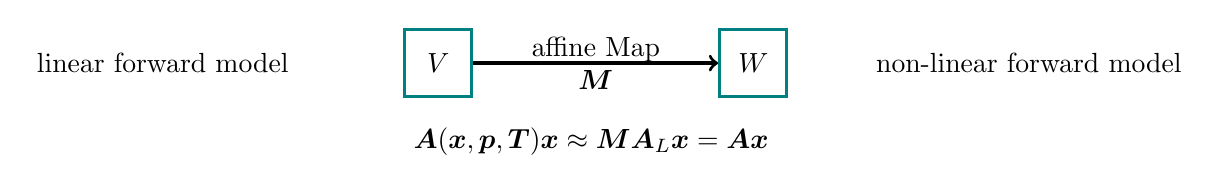
\begin{tikzpicture}
		\node[rectnode] at (2,-4) (NL)    {$W$};
		\node[rectnode] at (-2,-4) (L)    {$V$};
		\draw[<-, very thick] (NL.west) -- (L.east); 
		\node[align=center] at (-5.5,-4) (f3) {linear forward model};
		\node[align=center] at (5.5,-4) (f4) {non-linear forward model};
		\node[align=center] at (0,-5) (f5) {$\bm{A}(\bm{x},  \bm{p},\bm{T}) \bm{x}  \approx \bm{M A}_L  \bm{x} = \bm{A x} $ };
		\node[align=center] at (0,-4) (f5) {affine Map \\ $\bm{M}$};
	\end{tikzpicture}
	\caption[Schematics of Affine Map]{Schematics of Affine Map, which approximates the linear forward model to the non-linear forward model.}
\end{figure}

\section{Bayesian Inference}
Given some data $\bm{y}$, see Eq. \ref{}, from the Satellite limb sounder we like to use Bayesian inference to recover the parameter of iterest $\bm{x}$.
In doing so we set up a hierarchially order Bayesian model which naturally inlcudes hyperparameters $\bm{\theta}$, such as the radnom noise added to some obersovation from the space of all measurables $\bm{u}$.
This space is deterministicaly defined through the linear forward model $\bm{A}$.
We can visualize this hierarchial model through a directed acyclic graph (DAG), see Figure \ref{fig:FirstDAG}.

\begin{figure}[ht!]
	\centering
	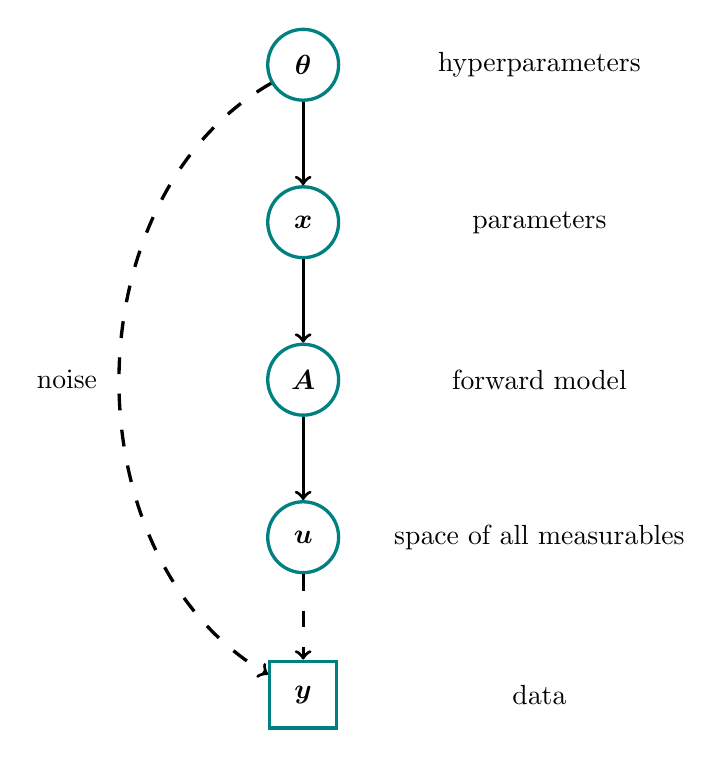
\begin{tikzpicture}
		\node[roundnode2] at (0,4) (th)    {$\bm{\theta}$};
		\node[roundnode2] at (0,2) (x)    {$\bm{x}$};
		\node[roundnode2] at (0,0) (A)    {$\bm{A}$};
		\node[roundnode2] at (0,-2) (u)    {$\bm{u}$};
		\node[rectnode] at (0,-4) (y)    {$\bm{y}$};

        \draw[->, very thick] (th.south) -- (x.north); 
        \draw[->, very thick] (x.south) -- (A.north); 
        \draw[->, very thick] (A.south) -- (u.north); 
        \draw[->, very thick, mydotted] (u.south) -- (y.north); 
        \draw[->, very thick, mydotted] (th) edge[bend right=60] (y);  
  
        \node[align=center] at (3,4) (tht) {hyperparameters};
        \node[align=center] at (3,2) (xt) {parameters};
        \node[align=center] at (3,0) (At) {forward model};
        \node[align=center] at (3,-2) (ut) {space of all measurables};
        \node[align=center] at (3,-4) (yt) {data};
        \node[align=center] at (-3,0) (nt) {noise};
	\end{tikzpicture}
	\caption[Bayesian Inference DAG]{The directed acyclic graph (DAG) for a typical linear inverse problem shows deterministic dependecys as solid line arrows and statistical dependencies as dotted arrows.
	Naturally the data $\bm{y}$ has some noise described through some hyperparameters $\bm{\theta}$ which determine the parameters $\bm{x}$. Those determine the space of all measurables $\bm{u}$ according to the forward model matrix $A$, so that $\bm{Ax}$ is a linear operation.
	From the space of all measurables we can observe some data $\bm{y}$, statistically, where as prevoiusly mentioned some random noise is added.
	We set up a more sophisticated Bayesian model in chapter \ref{} explicity including all hyper-parameters and parameters of interest.}
	\label{fig:FirstDAG}
\end{figure}

Within a linear Bayesian hierarchial model we need to define distribution over the unknown parameters and hyper-parameters
\begin{subequations}
	\begin{align}
		\bm{y}|\bm{x}, \bm{\theta}&\sim \mathcal{N}(\bm{A} \bm{x}, \bm{\Sigma}) \label{eq:likelihood}  \\
		\bm{x}| \bm{\theta} & \sim  \mathcal{N}( \bm{\mu}, \bm{Q}^{-1}  ) \label{eq:xPrior} \\
		\bm{\theta} &\sim  \pi(\bm{\theta}) \label{eq:gammaPrior}\, ,
	\end{align}
	\label{eq:BayMode}
\end{subequations}
with the noise covarince matrix $\bm{\Sigma}$, so that $\bm{\eta}  \sim \mathcal{N}(0, \bm{\Sigma}) $ as in Eq. \ref{}, the prior precision matrix $\bm{Q}$, prior mean $\bm{\mu}$
and some distribtion over the hyperparameters $\pi(\bm{\theta})$.
Then this becomes a linear-Gaussian Bayesian hierachial model.

According to Bayes' theorem we focus on the posterior distribution
\begin{align}
	\pi(\bm{x},\bm{\theta}|\bm{y}) = \frac{ \pi(\bm{y} | \bm{x}, \bm{\theta} ) \pi(\bm{x}, \bm{\theta})}{\pi(\bm{y})} \, ,
\end{align}
with the likelihood function $\pi(\bm{y} | \bm{x}, \bm{\theta} )$ and the prior distribution $\pi(\bm{x}, \bm{\theta})$.
If the normalizing contant $\pi(\bm{y})$ is fintie and non-zero we can approximate the posterior distribution
\begin{align}
	\pi(\bm{x},\bm{\theta}|\bm{y}) \propto \pi(\bm{y} | \bm{x}, \bm{\theta} ) \pi(\bm{x}, \bm{\theta}) \, .
\end{align}

Then the expecation of any a function $h(\bm{x})$ can be described as 
\begin{align}
	\text{E}_{\bm{x},\bm{\theta}|\bm{y}} [h(\bm{x})] =  \int \int   h(\bm{x}) \,  \pi(\bm{x}, \bm{\theta} | \bm{y} ) \, \text{d} \bm{x}  \, \text{d} \bm{\theta}   \label{eq:expPos} \, ,
\end{align}
which is usually a high dimensional integral and computationally not feasible to solve.

One way to work around the high dimensionality is to parameterize $\bm{x}$ using hyperparmaters $\bm{\theta}$ so that $\bm{x}(\bm{\theta})$. 
Another way is to seperate the posterior distribution over latent field $\bm{x}$ and the hyperparameters $\bm{\theta}$.
This is particular benefitial, when $\bm{x}$ is high dimesnional, e.g. $\bm{x} \in \mathbb{R}^n$ with $n = 45$, and can not be parameterized, and $\bm{\theta}$ is low dimensional, e.g. two dimensional.


\subsection{Marginal and then Conditional}
The marginal and then conditional (MTC) method factorizes the full posterior distribution 
\begin{align}
	\pi(\bm{x}, \bm{\theta}|\bm{y}) = \pi(\bm{x}| \bm{\theta}, \bm{y}) \pi(\bm{\theta}|\bm{y})
\end{align}
into the marginal posterior distribtion $ \pi(\bm{\theta}|\bm{y})$ and conditional posterior distribution $\pi(\bm{x}| \bm{\theta}, \bm{y})$.


For the in Eq. \ref{} specified linear-Gaussian Bayesian hierarchial model the marginal posterior distribution is given as
\begin{align}
	\pi(\bm{\theta} | \bm{y}) &= \int \pi(\bm{x}, \bm{\theta} | \bm{y}) \diff \bm{x} \\ 
	\label{eq:condHyper}
	&\propto \sqrt{ \frac{ \det( \bm{\Sigma}^{-1} ) \,  \det( \bm{Q}) }{\det( \bm{Q} + \bm{A}^T \bm{\Sigma}^{-1} \bm{A} ) } } \times \exp \Big[ - \frac{1}{2}(\bm{y} -\bm{A \mu})^T \bm{Q}_{\bm{\theta|y}} (\bm{y} -\bm{A \mu}) \Big] \pi(\bm{\theta}) \, ,
\end{align}
with
\begin{align}
	\bm{Q}_{\bm{\theta|y}} = \bm{\Sigma}^{-1} - \bm{\Sigma}^{-1} \bm{A} (\bm{A}^T \bm{\Sigma}^{-1} \bm{A} + \bm{Q} )^{-1} \bm{A}^T \bm{\Sigma}^{-1} \,  .
\end{align}
See lemma \cite{}.

Then conditioned on the hyperparameters $\bm{\theta}$ we can draw samples of the conditional posterior distribution
\begin{align}
	\bm{x}| \bm{y} , \bm{\theta} \sim \mathcal{N}\big( \bm{\mu} + (\bm{A}^T \bm{\Sigma}^{-1} \bm{A} + \bm{Q} )^{-1} \bm{A}^T \bm{\Sigma}^{-1} (\bm{y} - \bm{A} \bm{\mu}), (\bm{A}^T \bm{\Sigma}^{-1} \bm{A} + \bm{Q} )^{-1} \big) \, ,
\end{align}
see section \ref{} or caculate weighted expections of a function $h(\bm{x})$
\begin{align}
	\label{eq:lte}
	\text{E}_{\bm{x}|\bm{y}} [h(\bm{x})] = \int   \text{E}_{\bm{x}|\bm{\theta},\bm{y}} [h(\bm{x})] \, \pi(\bm{\theta} | \bm{y} )  \, \text{d} \bm{\theta} \,  ,
\end{align}
with weights given by $\pi(\bm{\theta} | \bm{y} )$.
\cite{}

In this thesis we will use sampling and deterministic methods to characterise the posterior distribtion over the hyperparameters and present the basics of those in the following sections.


\section{Sampling Methods -- MCMC}
The aim of sampling methods is to draw enough samples from the distribution of interest so that
the distrnution can characterised with sample based methods
Here we present the sampling methods/algorithms we are using.
Generating a Markov-Chain $ (\bm{x}, \bm{\theta} )^{(0)}, \dots, (\bm{x}, \bm{\theta} )^{(k)} , \dots,  (\bm{x}, \bm{\theta})^{(N)} \sim \pi(\bm{x},\bm{\theta}| \bm{y}) $ we accept and reject proposed samples to accurately calculate the sample mean.
Ergodicity

\begin{align}
	\label{eq:sampMean}
	\text{E}_{\bm{x},\bm{\theta}|\bm{y}} [h(\bm{x})] \approx \frac{1}{N} \sum_{k=1}^{N} h (\bm{x}^{(k)}) \, ,
\end{align}

\subsection{Metropolis}
Metropolis algorithm is special case of the Metropolis-Hastings algorithm, with a symmetric proposal distribution $q(\cdot|\cdot)$ \cite{}.

\begin{align}
\alpha(\bm{\theta}^{(t)}  | \bm{\theta}^{(t-1)}) = \min \left\{ 1, \frac{\pi(\bm{\theta}^{(t)}  | \bm{y}) \cdot 	q(\bm{\theta}^{(t-1)} | \bm{\theta})}{\pi(\bm{\theta}^{(t-1)}|  \bm{y}) \cdot q(\bm{\theta} | \bm{\theta}^{(t-1)})} \right\}= \min \left\{ 1, \frac{\pi(\bm{\theta}^{(t)}  | \bm{y}) }{\pi(\bm{\theta}^{(t-1)}| \bm{y})} \right\}
\end{align}

\begin{algorithm}
	\caption{Metropolis}
	\begin{algorithmic}[1]
		\STATE Initialize \( \bm{\theta}^{(0)} \).
		\FOR{ \( k = 1, \dots, N \)}
		\STATE Propose \( \bm{\theta}^{(t)} \sim \mathcal{N}(\bm{\theta} | \bm{\theta}^{(t-1)}) \)
		\STATE Compute
			\[ \alpha(\bm{\theta}^{(t)} | \bm{\theta}^{(t-1)}) = \min \left\{ 1, \frac{\pi(\bm{\theta}^{(t)}  | \bm{y}) }{\pi(\bm{\theta}^{(t-1)}| \bm{y}) } \right\} \]
		\STATE Accept and set \( \bm{\theta}^{(t)} = \bm{\theta} \) with probability \( \alpha(\bm{\theta}^{(t)}  | \bm{\theta}^{(t-1)}) \), otherwise set \(\bm{\theta}^{(t)} = \bm{\theta}^{(t-1)} \).
		\ENDFOR
	\end{algorithmic}
\end{algorithm}

\subsection{Gibbs}
\begin{algorithm}
	\caption{Gibbs}
	\begin{algorithmic}[1]
		\STATE Initialize \( \bm{\theta}^{(0)} = \{\bm{\theta}^{(0)}_{1}, \dots, \bm{\theta}^{(0)}_{j},\dots,\bm{\theta}^{(0)}_{d} \} \).
		\FOR{ \( k = 1, \dots, N \)}
		\FOR{ \( j = 1, \dots, d \)}
		\STATE Draw \(\bm{\theta}_j^{(t)} \sim  \pi(\bm{\theta}_j | \bm{\theta}_{<j}, \bm{\theta}_{>j} , \bm{y} )\) 

		\ENDFOR
		\ENDFOR
	\end{algorithmic}
\end{algorithm}

$ \bm{\theta}_{<j} = \{\bm{\theta}_{1}, \dots, \bm{\theta}_{j-1} \} $ 
$ \bm{\theta}_{>j} = \{\bm{\theta}_{j+1}, \dots, \bm{\theta}_{d}\} $which denotes all dimesnions except $ \bm{\theta}_{j}$
\subsection{t-walk}
We use the t-walk sampler as a black box sampling algorithm
\cite{}, so it prodices a ergodic markov chain


\subsection{Draw a sample from the Conditional posterior distribution -- RTO}
In the case of marginalising out the latent field we use a smaple of choice to genrate a amrkov chain.
Then we can draw a sample from that markov chain and condition on it so that we can draw a sample from the 
As the full conditional distribution for $\bm{x}| \bm{y} , \bm{\theta} $ is a normal distribution we can rewrite to:
\begin{align}
	\pi(\bm{x}|\bm{y}, \bm{\theta} ) &\propto \pi(\bm{y} | \bm{x} , \bm{\theta} ) \pi(\bm{x}| \bm{\theta}) \\
	&= \exp  \lVert \hat{\bm{A}} \bm{x} - \hat{\bm{y}} \rVert^2 \, ,
\end{align}
where 
\begin{align}
	\label{eq:minimizer}
	\hat{\bm{A}} = 
	\begin{bmatrix}
		\bm{\Sigma}^{-1/2}(\bm{\theta})  \bm{A}\\
		\bm{Q}^{1/2}(\bm{\theta}) 
	\end{bmatrix} \, , \quad \hat{\bm{y}} = 
	\begin{bmatrix}
		\bm{\Sigma}^{-1/2}(\bm{\theta})  \bm{y} \\
		\bm{Q}^{1/2}(\bm{\theta}) \bm{\mu}
	\end{bmatrix} \, .
\end{align}
One sample from the posterior can be computed by minimizing the following equation with respect to $\hat{\bm{x}}$ :
\begin{align}
	\bm{x}_i = \arg \min_{\hat{\bm{x}}} \lVert \hat{\bm{A}} \hat{\bm{x}} - ( \hat{\bm{y}} + \bm{\eta} ) \rVert^2 , \quad \bm{\eta} \sim \mathcal{N}(\bm{0}, \mathbf{I}) \, ,
\end{align}
where we add a randomized perturbation $\bm{\eta}$.
Next, we substitute $ - \hat{\bm{A}}^T  \bm{\eta}  = \bm{v}_1 + \bm{v}_2$ we can rewrite the argument of Eq. \ref{eq:minimizer} to 
\begin{align}
	\label{eq:RTO}
	(\bm{A}^T \bm{\Sigma}^{-1} \bm{A}+
	\bm{Q} ) \bm{x}_i &= \bm{A}^T \bm{\Sigma}^{-1} \bm{y} +  \bm{Q} \bm{\mu} + \bm{v}_1 + \bm{v}_2 \,  ,
\end{align}
where $\bm{v}_1 \sim \mathcal{N}(\bm{0}, \bm{A}^T \bm{\Sigma}^{-1} \bm{A}) $ and $\bm{v}_2 \sim \mathcal{N}(\bm{0}, \bm{Q} )$ are independent random variables.
Finally, we can draw an independent sample from the posterior $(\bm{x}_i, \bm{\theta}_i) \sim \pi(\bm{x}, \bm{\theta} | \bm{y})$.


\section{Numerical Approxiamtion Methods}
To approximate multi dimesnioan functions we can use the tensor train format to approximate marginal funcitons



\subsection{Tensor Train}

One of the main contributions of this paper is to show that the conditional distribution method is feasible, and efficient, once a PDF has been put into TT format. This section presents those calculations.

First, we describe the computation of the marginal PDFs \( p_k \), defined in (2), given \( \pi \) in a TT format (3). Note that integrals over the variable \( x_k \) appear in all conditionals (2) with \( k < d \). The TT format allows computing the \( r_{k-1} \times 1 \) vector \( P_k \) required for evaluating the marginal PDF \( p_{k-1} \) by the following algorithm:

\begin{algorithm}
	\caption{Computation of marginal PDFs}
	\begin{algorithmic}[1]
		\STATE Initialize \( P_{d+1} = 1 \).
		\FOR{ \( k = d, d-1, \dots, 2 \)}
		\STATE Compute
		\[
		(P_k)_{\alpha_{k-1}} =
		\sum_{\alpha_k=1}^{r_k} \left( \int_{\mathbb{R}} \pi^{(k)}_{\alpha_{k-1},\alpha_k} (x_k) \, dx_k \right) (P_{k+1})_{\alpha_k}
		\]
		\ENDFOR
	\end{algorithmic}
\end{algorithm}

Since \( \pi^{(k)}(x_k) \in \mathbb{R}^{r_{k-1} \times r_k} \) for each fixed \( x_k \), the integral \( \int \pi^{(k)}(x_k)dx_k \) is a \( r_{k-1} \times r_k \) matrix, where \( \alpha_{k-1} \) is the row index and \( \alpha_k \) is the column index. Hence, we can write Line 3 as the matrix–vector product:

\[
P_k = \left( \int_{\mathbb{R}} \pi^{(k)}(x_k)dx_k \right) P_{k+1}.
\]

Assuming \( n \) quadrature points for each \( x_k \), and the uniform rank bound \( r_k \leq r \), the asymptotic complexity of this algorithm is \( O(dnr^2) \).

The first marginal PDF is approximated by \( p^*_1(x_1) = |\pi^{(1)}(x_1) P_2| \). We take the absolute value because the TT approximation \( \pi^* \) (and hence, \( \pi^{(1)}(x_1) P_2 \)) may be negative at some locations. In the \( k \)-th step of the sampling procedure, the marginal PDF also requires the first \( k-1 \) TT blocks, restricted to the components of the sample that are already determined:

\[
p^*_k(x_1, \dots, x_{k-1}|x_k) = \left| \pi^{(1)}(x_1) \cdots \pi^{(k-1)}(x_{k-1}) \pi^{(k)}(x_k) P_{k+1} \right|.
\]

However, since the loop goes sequentially from \( k = 1 \) to \( k = d \), the sampled TT blocks can be accumulated in the same fashion as the integrals \( P_k \). Again, we take the absolute value to ensure positivity.

The \textbf{full} marginals are then defined as:
\[
p^*_k(x_k) = \left|  \left( \int_{\mathbb{R}} \pi^{(1)}(x_1)dx_{1} \right) \cdots \left( \int_{\mathbb{R}} \pi^{(k-1)}(x_{k-1})dx_{k-1} \right)  \pi^{(k)}(x_k) \left( \int_{\mathbb{R}} \pi^{(k+1)}(x_{k+1})dx_{k+1} \right) \cdots  \left( \int_{\mathbb{R}} \pi^{(d)}(x_d)dx_{d} \right) \right|.
\]

\section{SIRT - Marginal Functions and Conditional PDFs}
We represent each TT core of the decomposition in (18) as
\begin{equation}
	G^{(\alpha_{k-1},\alpha_k)}_k(x_k) = \sum_{i=1}^{n_k} \phi^{(i)}_k(x_k) \bm{A}_k[\alpha_{k-1}, i, \alpha_k], \quad k = 1, ..., d,
\end{equation}
where $\{\phi^{(i)}_k(x_k)\}_{i=1}^{n_k}$ is the set of basis functions for the $k$-th coordinate and $\bm{A}_k \in \mathbb{R}^{r_{k-1} \times n_k \times r_k}$ is the associated $k$-th coefficient tensor. For the $k$-th set of basis functions, we define the mass matrix $\bm{M}_k \in \mathbb{R}^{n_k \times n_k}$ by
\begin{equation}
	\bm{M}_k[i, j] = \int_{X_k} \phi^{(i)}_k(x_k) \phi^{(j)}_k(x_k) \lambda(x_k) \,dx_k, \quad i = 1, ..., n_k, \quad j = 1, ..., n_k.
\end{equation}


\section{right to left}

\begin{prop}
	Starting with the last coordinate $k = d$, we set $\bm{B}_d = \bm{A}_d$. Suppose for the first $k$ dimensions ($d > k\geq  1$), we have a coefficient tensor $\bm{B}_k \in \mathbb{R}^{r_{k-1} \times n_k \times r_k}$ that defines a marginal function $\pi_{\leq k}(x_{\leq k})$ as in (??). The following procedure \textbf{can} be used to obtain the coefficient tensor $\bm{B}_{k-1} \in \mathbb{R}^{r_{k-2} \times n_{k-1} \times r_{k-1}}$ for defining the next marginal function $\pi_{<k}(x_{<k})$:
	\begin{enumerate}
		\item Use the Cholesky decomposition of the mass matrix, $\bm{L}_k \bm{L}_k^\top = \bm{M}_k \in \mathbb{R}^{n_k \times n_k}$, to construct a tensor $\bm{C}_k \in \mathbb{R}^{r_{k-1} \times n_k \times r_k}$:
		\begin{equation}
			\bm{C}_k[\alpha_{k-1}, \tau, l_k] = \sum_{i=1}^{n_k} \bm{B}_k[\alpha_{k-1}, i, l_k] \bm{L}_k[i, \tau].
		\end{equation}
		\item Unfold $\bm{C}_k$ along the first coordinate and compute the thin QR decomposition, so that $\bm{C}_k^{(R)} \in \mathbb{R}^{r_{k-1} \times (n_k r_k)}$:
		\begin{equation}
			\bm{Q}_k \bm{R}_k = {(\bm{C}_k^{(R)})}^{\top}.
		\end{equation}
		\item Compute the new coefficient tensor:
		\begin{equation}
			\bm{B}_{k-1}[\alpha_{k-2}, i, l_{k-1}] = \sum_{\alpha_{k-1}=1}^{r_{k-1}} \bm{A}_{k-1}[\alpha_{k-2}, i, \alpha_{k-1}] \bm{R}_k[l_{k-1}, \alpha_{k-1}].
		\end{equation}
	\end{enumerate}
\end{prop}





\section{left to right}

\begin{prop}
	Starting with the first coordinate $k = 1$, we set $\bm{B}_{pre,1} = \bm{A}_1$. Suppose for the last $k$ dimensions ($k < d$), we have a coefficient tensor $\bm{B}_{pre,k} \in \mathbb{R}^{r_{k-1} \times n_k \times r_k}$ that defines a marginal function $\pi_{\leq k}(x_{\leq k})$ as in (??). The following procedure \textbf{can} be used to obtain the coefficient tensor $\bm{B}_{pre,k+1} \in \mathbb{R}^{r_{k} \times n_{k+1} \times r_{k+1}}$ for defining the next marginal function $\pi_{>k}(x_{>k})$:
	\begin{enumerate}
		\item Use the Cholesky decomposition of the mass matrix, $\bm{L}_k \bm{L}_k^\top = \bm{M}_k \in \mathbb{R}^{n_k \times n_k}$, to construct a tensor $\bm{C}_k \in \mathbb{R}^{r_{k-1} \times n_k \times r_k}$:
		\begin{equation}
			\bm{C}_{pre,k}[\alpha_{k-1}, \tau, l_k] = \sum_{i=1}^{n_k} \bm{L}_k[i, \tau] \bm{B}_{pre,k}[\alpha_{k-1}, i, l_k] .
		\end{equation}
		\item Unfold $\bm{C}_{pre,k}$ along the first coordinate and compute the thin QR decomposition, so that $\bm{C}_{pre,k}^{(R)} \in \mathbb{R}^{(r_{k-1} n_k ) \times r_k}$:
		\begin{equation}
			\bm{Q}_{pre,k}\bm{R}_{pre,k} = {(\bm{C}_{pre,k}^{(R)})}.
		\end{equation}
		\item Compute the new coefficient tensor $\bm{B}_{pre, k+1} \in \mathbb{R}^{r_{k-1} \times n_k \times r_k} $:
		\begin{equation}
			\bm{B}_{pre, k+1}[l_{k+1}, i, \alpha_{k+1}] = \sum_{\alpha_{k}=1}^{r_{k}} \bm{R}_{pre,k}[l_{k+1}, \alpha_{k}] \bm{A}_{k+1}[\alpha_{k}, i, \alpha_{k+1}] .
		\end{equation}
	\end{enumerate}
\end{prop}
\section{Calc Marginals}
\begin{prop}
	The marginal PDF of $X_1$ can be expressed as
	\begin{equation}
		f_{X_1}(x_1) = \frac{1}{z} \left(\gamma \prod_{i=2}^{d} \lambda_i(X_i) + \sum_{l_1=1}^{r_1} \left(\sum_{i=1}^{n_1} \phi^{(i)}_1(x_1) \bm{D}_1[i, l_1] \right)^2 \right) \lambda_1(x_1),
	\end{equation}
	where $\bm{D}_1[i, l_1] = \bm{B}_1[\alpha_0, i, l_1]$ and $\alpha_0 = 1$.\\
	The marginal PDF of $X_n$ can be expressed as
	\begin{equation}
		f_{X_n}(x_n) = \frac{1}{z} \left(\gamma \prod_{i=1}^{d-1} \lambda_i(X_i) + \sum_{l_{n-1}=1}^{r_{n-1}} \left(\sum_{i=1}^{n_1} \phi^{(i)}_1(x_1) \bm{D}_n[l_{n-1},i] \right)^2 \right) \lambda_n(x_n),
	\end{equation}
	where $\bm{D}_n[l_{n-1},i] = \bm{B}_{pre,n}[l_{n-1}, i, \alpha_n]$ and $\alpha_n = 1$.
	
	The marginal PDF of $X_{k}$ can be expressed as
	\begin{equation}
		f_{X_k}(x_k) = \frac{1}{\pi_{<k}(x_{<k}) \pi_{>k}(x_{>k})} \left(\gamma \prod_{i=1}^{k-1} \lambda_i(X_i) \prod_{i=k+1}^{d} \lambda_i(X_i) + \sum_{l_{k-1}=1}^{r_{k-1}} \sum_{l_k=1}^{r_k} \left(\sum_{i=1}^{n_k} \phi^{(i)}_k(x_k) \bm{D}_k[l_{k-1},i, l_k] \right)^2 \right) \lambda_k(x_k),
	\end{equation}
	where $\bm{D}_k \in \mathbb{R}^{r_{k-1} \times n_k \times r_k}$ and $\bm{R}_{pre,k-1}\in \mathbb{R}^{r_{k-1} \times r_{k-1}}$ and $\bm{B}_k \in \mathbb{R}^{r_{k-1} \times n_k \times r_k}$
	\begin{equation}
		\bm{D}_k[l_{k-1},i,l_k] = \sum_{\alpha_{k-1}=1}^{r_{k-1}}  \bm{R}_{pre,k-1}[l_{k-1}, \alpha_{k-1}] \bm{B}_k[\alpha_{k-1}, i, l_k].
	\end{equation}
\end{prop}



%
\chapter{Building a physics based hierarchical Linear model}
\begin{itemize}
	\item two hyperparameters, marginal and then conditonal, MTC, use as a building block \cite{fox2016fast, rue2005gaussian}
	\item  sampling, Gibbs-MH, t-walk \cite{christen2010general}
	\item increase hyperparameters, Temperature and pressure, tt-approx, SIRT \cite{cui2022deep, atmosphere1976us}
\end{itemize}

\section{Linear model}
\begin{itemize}
	\item define model \cite{readings2000envisat}
	\item explain parameters and constants \cite{gordon2022hitran2020}
	\item how pressure to height and temperature hydro-static equilibrium equation \cite{atmosphere1976us}
\end{itemize}

\section{two hyperameters, fast sampling paper}
\begin{itemize}
	\item similar to MTC paper,  \cite{fox2016fast}
	\item can compare to regularization and can integrate easily with less solves to regularization or RTO, \cite{hansen1993use}
	\item define priors make table
	\item how many steps, integrated autocorrealtion time , ref
	\item relative error
	\item how I found max curvature, \cite{satopaa2011kneedle}
	\item how many taylor series
\end{itemize}

\begin{figure}[thb!]
	\centering
	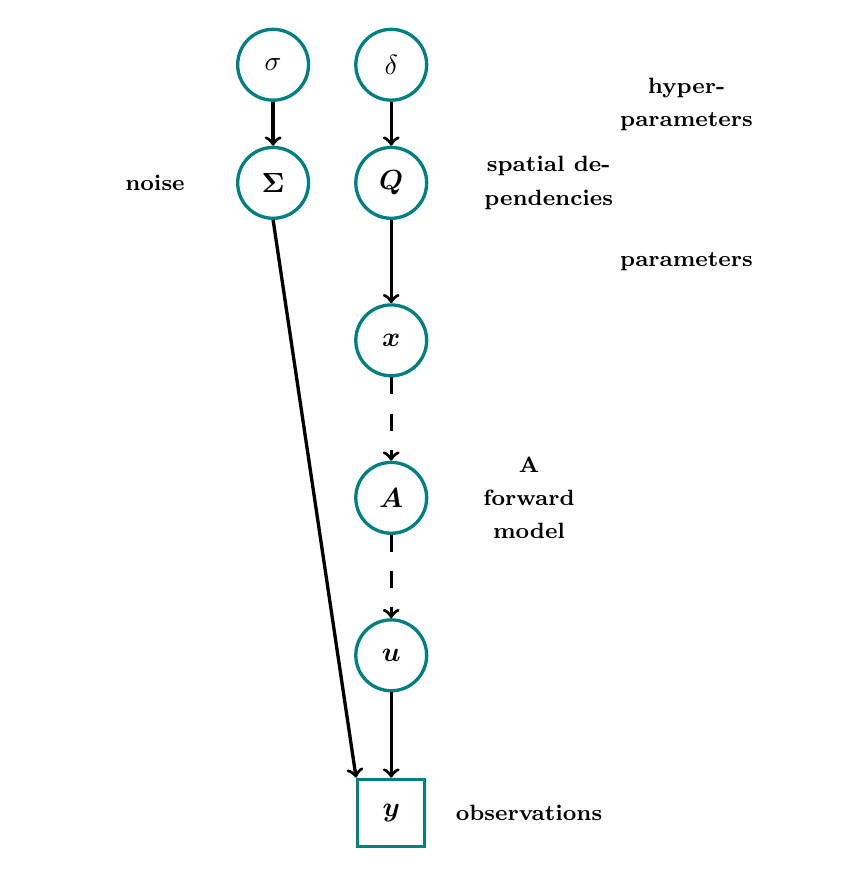
\begin{tikzpicture}
		\node[roundnode2] at (0,6) (Q)     {$\bm{Q}$};
		\node[roundnode2] at (0,4) (x)     {$\bm{x}$};
		\node[roundnode2] at (0,2) (A)    {$\bm{A}$};
		\node[roundnode2] at (0,0) (u)    {$\bm{u}$};
		\node[rectnode] at (0,-2) (y)    {$\bm{y}$};
		\node[roundnode2] at (-1.5,6) (S)    {$\bm{\Sigma}$};
		\node[roundnode2] at (-1.5,7.5) (s)    {$\sigma$};
		\node[roundnode2] at (0,7.5) (d)    {$\delta$};
		
		%text
		%\draw (-1,2.5) node[align=center, text width=1.5cm] {\footnotesize \textbf{hydrostatic \\ equation}};
		\draw (1.75,2) node[align=center, text width=1.5cm] {\footnotesize \textbf{A \\ forward model }};
		%\draw (6.75,-1.5) node[align=center, text width=2.5cm] {\footnotesize \textbf{hyper\-parameters}};
		%\draw (5.5,-1.5) node[align=center, text width=0.5cm] { $\bm{\theta}$};
		\draw (1.75,-2) node[align=center, text width=3cm] {\footnotesize \textbf{observations}};
		\draw (3.75,7) node[align=center, text width=3cm] {\footnotesize \textbf{hyper-\\parameters}};
		\draw (3.75,5) node[align=center, text width=3cm] {\footnotesize \textbf{parameters}};
		\draw (2,6) node[align=center, text width=3cm] {\footnotesize \textbf{spatial dependencies}};
		%\draw (-1.4,-2.3) node[align=center, text width=3cm] {\footnotesize \textbf{hyper-prior}};
		\draw (-3,6) node[align=center, text width=3cm] {\footnotesize \textbf{noise}};
		% Calligraphic brace
		%\draw[very thick, decorate,decoration = {brace}] (5,-1) --  (5,-2);
		
		%Lines
		\draw[->, very thick] (S.south) -- (y.north west);
		\draw[->, very thick] (s.south) -- (S.north);
		\draw[->, very thick] (u.south) -- (y.north);
		\draw[->, mydotted, very thick] (A.south) -- (u.north);
		\draw[->, mydotted,  very thick] (x.south) -- (A.north);
		
		\draw[->, very thick] (d.south) -- (Q.north); 
		\draw[->, very thick] (Q.south) -- (x.north); 
		
		
	\end{tikzpicture} 
	\caption[]{}
\end{figure}

\begin{figure}[!ht]
	\centering
	\renewcommand\sffamily{}
	\renewcommand{\mathbf}{\bm}
	%\includegraphics[width = 0.99\columnwidth]{f_and_g_paper.png}
	\scalebox{0.66}{\input{f_and_g_paper.pdf_tex}}
	%\input{f_and_g_paper.pdf_tex}
	\caption{Functions $f(\lambda)$, dotted, and $g(\lambda)$, dashed, of the marginal posterior distribution for the specific forward model used in this study. Both functions are well-behaved over a large range of $\lambda$. In the support region of the MWG the pink square refers to the mode of the marginal posterior. Additionally, we plot the Taylor series of fourth order for $f(\lambda)$ and $g(\lambda)$ around the mode, see black line.}
	\label{fig:f_and_g}
\end{figure}

\begin{figure}[!ht]
	\centering
	\renewcommand\sffamily{}
	\renewcommand{\mathbf}{\bm}
	%\scalebox{0.66}{\input{AllHistoResults.pgf}}
	\scalebox{0.66}{%% Creator: Matplotlib, PGF backend
%%
%% To include the figure in your LaTeX document, write
%%   \input{<filename>.pgf}
%%
%% Make sure the required packages are loaded in your preamble
%%   \usepackage{pgf}
%%
%% Also ensure that all the required font packages are loaded; for instance,
%% the lmodern package is sometimes necessary when using math font.
%%   \usepackage{lmodern}
%%
%% Figures using additional raster images can only be included by \input if
%% they are in the same directory as the main LaTeX file. For loading figures
%% from other directories you can use the `import` package
%%   \usepackage{import}
%%
%% and then include the figures with
%%   \import{<path to file>}{<filename>.pgf}
%%
%% Matplotlib used the following preamble
%%   
%%   \makeatletter\@ifpackageloaded{underscore}{}{\usepackage[strings]{underscore}}\makeatother
%%
\begingroup%
\makeatletter%
\begin{pgfpicture}%
\pgfpathrectangle{\pgfpointorigin}{\pgfqpoint{4.920000in}{4.920000in}}%
\pgfusepath{use as bounding box, clip}%
\begin{pgfscope}%
\pgfsetbuttcap%
\pgfsetmiterjoin%
\definecolor{currentfill}{rgb}{1.000000,1.000000,1.000000}%
\pgfsetfillcolor{currentfill}%
\pgfsetlinewidth{0.000000pt}%
\definecolor{currentstroke}{rgb}{1.000000,1.000000,1.000000}%
\pgfsetstrokecolor{currentstroke}%
\pgfsetdash{}{0pt}%
\pgfpathmoveto{\pgfqpoint{0.000000in}{0.000000in}}%
\pgfpathlineto{\pgfqpoint{4.920000in}{0.000000in}}%
\pgfpathlineto{\pgfqpoint{4.920000in}{4.920000in}}%
\pgfpathlineto{\pgfqpoint{0.000000in}{4.920000in}}%
\pgfpathlineto{\pgfqpoint{0.000000in}{0.000000in}}%
\pgfpathclose%
\pgfusepath{fill}%
\end{pgfscope}%
\begin{pgfscope}%
\pgfsetbuttcap%
\pgfsetmiterjoin%
\definecolor{currentfill}{rgb}{1.000000,1.000000,1.000000}%
\pgfsetfillcolor{currentfill}%
\pgfsetlinewidth{0.000000pt}%
\definecolor{currentstroke}{rgb}{0.000000,0.000000,0.000000}%
\pgfsetstrokecolor{currentstroke}%
\pgfsetstrokeopacity{0.000000}%
\pgfsetdash{}{0pt}%
\pgfpathmoveto{\pgfqpoint{0.854238in}{2.092082in}}%
\pgfpathlineto{\pgfqpoint{4.820000in}{2.092082in}}%
\pgfpathlineto{\pgfqpoint{4.820000in}{4.820000in}}%
\pgfpathlineto{\pgfqpoint{0.854238in}{4.820000in}}%
\pgfpathlineto{\pgfqpoint{0.854238in}{2.092082in}}%
\pgfpathclose%
\pgfusepath{fill}%
\end{pgfscope}%
\begin{pgfscope}%
\pgfpathrectangle{\pgfqpoint{0.854238in}{2.092082in}}{\pgfqpoint{3.965762in}{2.727918in}}%
\pgfusepath{clip}%
\pgfsetbuttcap%
\pgfsetroundjoin%
\definecolor{currentfill}{rgb}{0.000000,0.000000,0.000000}%
\pgfsetfillcolor{currentfill}%
\pgfsetlinewidth{1.003750pt}%
\definecolor{currentstroke}{rgb}{0.000000,0.000000,0.000000}%
\pgfsetstrokecolor{currentstroke}%
\pgfsetdash{}{0pt}%
\pgfsys@defobject{currentmarker}{\pgfqpoint{-0.020833in}{-0.020833in}}{\pgfqpoint{0.020833in}{0.020833in}}{%
\pgfpathmoveto{\pgfqpoint{0.000000in}{-0.020833in}}%
\pgfpathcurveto{\pgfqpoint{0.005525in}{-0.020833in}}{\pgfqpoint{0.010825in}{-0.018638in}}{\pgfqpoint{0.014731in}{-0.014731in}}%
\pgfpathcurveto{\pgfqpoint{0.018638in}{-0.010825in}}{\pgfqpoint{0.020833in}{-0.005525in}}{\pgfqpoint{0.020833in}{0.000000in}}%
\pgfpathcurveto{\pgfqpoint{0.020833in}{0.005525in}}{\pgfqpoint{0.018638in}{0.010825in}}{\pgfqpoint{0.014731in}{0.014731in}}%
\pgfpathcurveto{\pgfqpoint{0.010825in}{0.018638in}}{\pgfqpoint{0.005525in}{0.020833in}}{\pgfqpoint{0.000000in}{0.020833in}}%
\pgfpathcurveto{\pgfqpoint{-0.005525in}{0.020833in}}{\pgfqpoint{-0.010825in}{0.018638in}}{\pgfqpoint{-0.014731in}{0.014731in}}%
\pgfpathcurveto{\pgfqpoint{-0.018638in}{0.010825in}}{\pgfqpoint{-0.020833in}{0.005525in}}{\pgfqpoint{-0.020833in}{0.000000in}}%
\pgfpathcurveto{\pgfqpoint{-0.020833in}{-0.005525in}}{\pgfqpoint{-0.018638in}{-0.010825in}}{\pgfqpoint{-0.014731in}{-0.014731in}}%
\pgfpathcurveto{\pgfqpoint{-0.010825in}{-0.018638in}}{\pgfqpoint{-0.005525in}{-0.020833in}}{\pgfqpoint{0.000000in}{-0.020833in}}%
\pgfpathlineto{\pgfqpoint{0.000000in}{-0.020833in}}%
\pgfpathclose%
\pgfusepath{stroke,fill}%
}%
\begin{pgfscope}%
\pgfsys@transformshift{2.043625in}{3.407497in}%
\pgfsys@useobject{currentmarker}{}%
\end{pgfscope}%
\begin{pgfscope}%
\pgfsys@transformshift{2.119751in}{3.269421in}%
\pgfsys@useobject{currentmarker}{}%
\end{pgfscope}%
\begin{pgfscope}%
\pgfsys@transformshift{1.707597in}{3.049194in}%
\pgfsys@useobject{currentmarker}{}%
\end{pgfscope}%
\begin{pgfscope}%
\pgfsys@transformshift{1.836575in}{3.246105in}%
\pgfsys@useobject{currentmarker}{}%
\end{pgfscope}%
\begin{pgfscope}%
\pgfsys@transformshift{2.290375in}{3.179193in}%
\pgfsys@useobject{currentmarker}{}%
\end{pgfscope}%
\begin{pgfscope}%
\pgfsys@transformshift{2.735692in}{3.183461in}%
\pgfsys@useobject{currentmarker}{}%
\end{pgfscope}%
\begin{pgfscope}%
\pgfsys@transformshift{2.566950in}{4.142220in}%
\pgfsys@useobject{currentmarker}{}%
\end{pgfscope}%
\begin{pgfscope}%
\pgfsys@transformshift{2.341331in}{2.929143in}%
\pgfsys@useobject{currentmarker}{}%
\end{pgfscope}%
\begin{pgfscope}%
\pgfsys@transformshift{3.158086in}{3.249298in}%
\pgfsys@useobject{currentmarker}{}%
\end{pgfscope}%
\begin{pgfscope}%
\pgfsys@transformshift{2.889926in}{3.079613in}%
\pgfsys@useobject{currentmarker}{}%
\end{pgfscope}%
\begin{pgfscope}%
\pgfsys@transformshift{1.380199in}{3.041342in}%
\pgfsys@useobject{currentmarker}{}%
\end{pgfscope}%
\begin{pgfscope}%
\pgfsys@transformshift{2.239076in}{3.570717in}%
\pgfsys@useobject{currentmarker}{}%
\end{pgfscope}%
\begin{pgfscope}%
\pgfsys@transformshift{2.191076in}{2.885952in}%
\pgfsys@useobject{currentmarker}{}%
\end{pgfscope}%
\begin{pgfscope}%
\pgfsys@transformshift{1.484597in}{3.796933in}%
\pgfsys@useobject{currentmarker}{}%
\end{pgfscope}%
\begin{pgfscope}%
\pgfsys@transformshift{1.845087in}{3.864137in}%
\pgfsys@useobject{currentmarker}{}%
\end{pgfscope}%
\begin{pgfscope}%
\pgfsys@transformshift{1.705888in}{2.807564in}%
\pgfsys@useobject{currentmarker}{}%
\end{pgfscope}%
\begin{pgfscope}%
\pgfsys@transformshift{2.399218in}{4.333028in}%
\pgfsys@useobject{currentmarker}{}%
\end{pgfscope}%
\begin{pgfscope}%
\pgfsys@transformshift{2.390499in}{3.708101in}%
\pgfsys@useobject{currentmarker}{}%
\end{pgfscope}%
\begin{pgfscope}%
\pgfsys@transformshift{1.659209in}{3.317853in}%
\pgfsys@useobject{currentmarker}{}%
\end{pgfscope}%
\begin{pgfscope}%
\pgfsys@transformshift{2.282336in}{3.159560in}%
\pgfsys@useobject{currentmarker}{}%
\end{pgfscope}%
\begin{pgfscope}%
\pgfsys@transformshift{1.865595in}{3.082888in}%
\pgfsys@useobject{currentmarker}{}%
\end{pgfscope}%
\begin{pgfscope}%
\pgfsys@transformshift{2.559741in}{3.364065in}%
\pgfsys@useobject{currentmarker}{}%
\end{pgfscope}%
\begin{pgfscope}%
\pgfsys@transformshift{2.627812in}{3.414607in}%
\pgfsys@useobject{currentmarker}{}%
\end{pgfscope}%
\begin{pgfscope}%
\pgfsys@transformshift{2.252661in}{2.779246in}%
\pgfsys@useobject{currentmarker}{}%
\end{pgfscope}%
\begin{pgfscope}%
\pgfsys@transformshift{2.465137in}{3.204093in}%
\pgfsys@useobject{currentmarker}{}%
\end{pgfscope}%
\begin{pgfscope}%
\pgfsys@transformshift{1.735209in}{3.578415in}%
\pgfsys@useobject{currentmarker}{}%
\end{pgfscope}%
\begin{pgfscope}%
\pgfsys@transformshift{1.516331in}{3.561104in}%
\pgfsys@useobject{currentmarker}{}%
\end{pgfscope}%
\begin{pgfscope}%
\pgfsys@transformshift{2.489923in}{3.300069in}%
\pgfsys@useobject{currentmarker}{}%
\end{pgfscope}%
\begin{pgfscope}%
\pgfsys@transformshift{2.530425in}{3.552916in}%
\pgfsys@useobject{currentmarker}{}%
\end{pgfscope}%
\begin{pgfscope}%
\pgfsys@transformshift{2.831219in}{3.647331in}%
\pgfsys@useobject{currentmarker}{}%
\end{pgfscope}%
\begin{pgfscope}%
\pgfsys@transformshift{2.609308in}{3.264935in}%
\pgfsys@useobject{currentmarker}{}%
\end{pgfscope}%
\begin{pgfscope}%
\pgfsys@transformshift{2.485345in}{3.122114in}%
\pgfsys@useobject{currentmarker}{}%
\end{pgfscope}%
\begin{pgfscope}%
\pgfsys@transformshift{2.731362in}{3.353346in}%
\pgfsys@useobject{currentmarker}{}%
\end{pgfscope}%
\begin{pgfscope}%
\pgfsys@transformshift{2.769397in}{3.504885in}%
\pgfsys@useobject{currentmarker}{}%
\end{pgfscope}%
\begin{pgfscope}%
\pgfsys@transformshift{1.987129in}{3.674076in}%
\pgfsys@useobject{currentmarker}{}%
\end{pgfscope}%
\begin{pgfscope}%
\pgfsys@transformshift{2.036893in}{2.702229in}%
\pgfsys@useobject{currentmarker}{}%
\end{pgfscope}%
\begin{pgfscope}%
\pgfsys@transformshift{2.296886in}{3.323460in}%
\pgfsys@useobject{currentmarker}{}%
\end{pgfscope}%
\begin{pgfscope}%
\pgfsys@transformshift{3.369148in}{2.830219in}%
\pgfsys@useobject{currentmarker}{}%
\end{pgfscope}%
\begin{pgfscope}%
\pgfsys@transformshift{2.290682in}{2.957613in}%
\pgfsys@useobject{currentmarker}{}%
\end{pgfscope}%
\begin{pgfscope}%
\pgfsys@transformshift{1.646551in}{4.131457in}%
\pgfsys@useobject{currentmarker}{}%
\end{pgfscope}%
\begin{pgfscope}%
\pgfsys@transformshift{1.683503in}{2.846457in}%
\pgfsys@useobject{currentmarker}{}%
\end{pgfscope}%
\begin{pgfscope}%
\pgfsys@transformshift{2.310535in}{3.037404in}%
\pgfsys@useobject{currentmarker}{}%
\end{pgfscope}%
\begin{pgfscope}%
\pgfsys@transformshift{2.067139in}{3.268506in}%
\pgfsys@useobject{currentmarker}{}%
\end{pgfscope}%
\begin{pgfscope}%
\pgfsys@transformshift{2.621473in}{3.088569in}%
\pgfsys@useobject{currentmarker}{}%
\end{pgfscope}%
\begin{pgfscope}%
\pgfsys@transformshift{2.930515in}{3.216203in}%
\pgfsys@useobject{currentmarker}{}%
\end{pgfscope}%
\begin{pgfscope}%
\pgfsys@transformshift{1.288864in}{3.029120in}%
\pgfsys@useobject{currentmarker}{}%
\end{pgfscope}%
\begin{pgfscope}%
\pgfsys@transformshift{2.195155in}{3.783760in}%
\pgfsys@useobject{currentmarker}{}%
\end{pgfscope}%
\begin{pgfscope}%
\pgfsys@transformshift{2.762095in}{3.546178in}%
\pgfsys@useobject{currentmarker}{}%
\end{pgfscope}%
\begin{pgfscope}%
\pgfsys@transformshift{2.796273in}{3.080077in}%
\pgfsys@useobject{currentmarker}{}%
\end{pgfscope}%
\begin{pgfscope}%
\pgfsys@transformshift{2.485281in}{4.510916in}%
\pgfsys@useobject{currentmarker}{}%
\end{pgfscope}%
\begin{pgfscope}%
\pgfsys@transformshift{1.613229in}{2.633496in}%
\pgfsys@useobject{currentmarker}{}%
\end{pgfscope}%
\begin{pgfscope}%
\pgfsys@transformshift{2.581159in}{3.388983in}%
\pgfsys@useobject{currentmarker}{}%
\end{pgfscope}%
\begin{pgfscope}%
\pgfsys@transformshift{2.360751in}{3.006697in}%
\pgfsys@useobject{currentmarker}{}%
\end{pgfscope}%
\begin{pgfscope}%
\pgfsys@transformshift{1.954994in}{3.343699in}%
\pgfsys@useobject{currentmarker}{}%
\end{pgfscope}%
\begin{pgfscope}%
\pgfsys@transformshift{3.141239in}{3.709168in}%
\pgfsys@useobject{currentmarker}{}%
\end{pgfscope}%
\begin{pgfscope}%
\pgfsys@transformshift{2.970675in}{3.309702in}%
\pgfsys@useobject{currentmarker}{}%
\end{pgfscope}%
\begin{pgfscope}%
\pgfsys@transformshift{2.585361in}{3.081317in}%
\pgfsys@useobject{currentmarker}{}%
\end{pgfscope}%
\begin{pgfscope}%
\pgfsys@transformshift{1.741575in}{4.071216in}%
\pgfsys@useobject{currentmarker}{}%
\end{pgfscope}%
\begin{pgfscope}%
\pgfsys@transformshift{1.790316in}{3.055721in}%
\pgfsys@useobject{currentmarker}{}%
\end{pgfscope}%
\begin{pgfscope}%
\pgfsys@transformshift{1.591922in}{2.911854in}%
\pgfsys@useobject{currentmarker}{}%
\end{pgfscope}%
\begin{pgfscope}%
\pgfsys@transformshift{1.760695in}{3.584190in}%
\pgfsys@useobject{currentmarker}{}%
\end{pgfscope}%
\begin{pgfscope}%
\pgfsys@transformshift{2.283656in}{3.668231in}%
\pgfsys@useobject{currentmarker}{}%
\end{pgfscope}%
\begin{pgfscope}%
\pgfsys@transformshift{1.961119in}{4.045434in}%
\pgfsys@useobject{currentmarker}{}%
\end{pgfscope}%
\begin{pgfscope}%
\pgfsys@transformshift{2.759996in}{3.258569in}%
\pgfsys@useobject{currentmarker}{}%
\end{pgfscope}%
\begin{pgfscope}%
\pgfsys@transformshift{1.489189in}{3.198395in}%
\pgfsys@useobject{currentmarker}{}%
\end{pgfscope}%
\begin{pgfscope}%
\pgfsys@transformshift{2.602335in}{3.321794in}%
\pgfsys@useobject{currentmarker}{}%
\end{pgfscope}%
\begin{pgfscope}%
\pgfsys@transformshift{2.189678in}{3.308873in}%
\pgfsys@useobject{currentmarker}{}%
\end{pgfscope}%
\begin{pgfscope}%
\pgfsys@transformshift{2.455038in}{3.983515in}%
\pgfsys@useobject{currentmarker}{}%
\end{pgfscope}%
\begin{pgfscope}%
\pgfsys@transformshift{2.143125in}{3.187013in}%
\pgfsys@useobject{currentmarker}{}%
\end{pgfscope}%
\begin{pgfscope}%
\pgfsys@transformshift{2.341635in}{2.989514in}%
\pgfsys@useobject{currentmarker}{}%
\end{pgfscope}%
\begin{pgfscope}%
\pgfsys@transformshift{1.912998in}{3.788686in}%
\pgfsys@useobject{currentmarker}{}%
\end{pgfscope}%
\begin{pgfscope}%
\pgfsys@transformshift{1.858034in}{3.853805in}%
\pgfsys@useobject{currentmarker}{}%
\end{pgfscope}%
\begin{pgfscope}%
\pgfsys@transformshift{1.279687in}{3.146293in}%
\pgfsys@useobject{currentmarker}{}%
\end{pgfscope}%
\begin{pgfscope}%
\pgfsys@transformshift{1.914353in}{3.144664in}%
\pgfsys@useobject{currentmarker}{}%
\end{pgfscope}%
\begin{pgfscope}%
\pgfsys@transformshift{2.290631in}{3.228443in}%
\pgfsys@useobject{currentmarker}{}%
\end{pgfscope}%
\begin{pgfscope}%
\pgfsys@transformshift{2.109041in}{2.854416in}%
\pgfsys@useobject{currentmarker}{}%
\end{pgfscope}%
\begin{pgfscope}%
\pgfsys@transformshift{2.190986in}{3.247594in}%
\pgfsys@useobject{currentmarker}{}%
\end{pgfscope}%
\begin{pgfscope}%
\pgfsys@transformshift{1.589699in}{3.240683in}%
\pgfsys@useobject{currentmarker}{}%
\end{pgfscope}%
\begin{pgfscope}%
\pgfsys@transformshift{1.969123in}{3.018591in}%
\pgfsys@useobject{currentmarker}{}%
\end{pgfscope}%
\begin{pgfscope}%
\pgfsys@transformshift{2.520378in}{3.355702in}%
\pgfsys@useobject{currentmarker}{}%
\end{pgfscope}%
\begin{pgfscope}%
\pgfsys@transformshift{2.463160in}{3.335061in}%
\pgfsys@useobject{currentmarker}{}%
\end{pgfscope}%
\begin{pgfscope}%
\pgfsys@transformshift{2.082641in}{3.641560in}%
\pgfsys@useobject{currentmarker}{}%
\end{pgfscope}%
\begin{pgfscope}%
\pgfsys@transformshift{2.049091in}{3.214446in}%
\pgfsys@useobject{currentmarker}{}%
\end{pgfscope}%
\begin{pgfscope}%
\pgfsys@transformshift{2.001095in}{3.462845in}%
\pgfsys@useobject{currentmarker}{}%
\end{pgfscope}%
\begin{pgfscope}%
\pgfsys@transformshift{2.110193in}{3.758457in}%
\pgfsys@useobject{currentmarker}{}%
\end{pgfscope}%
\begin{pgfscope}%
\pgfsys@transformshift{2.446627in}{3.107903in}%
\pgfsys@useobject{currentmarker}{}%
\end{pgfscope}%
\begin{pgfscope}%
\pgfsys@transformshift{2.620706in}{3.036273in}%
\pgfsys@useobject{currentmarker}{}%
\end{pgfscope}%
\begin{pgfscope}%
\pgfsys@transformshift{3.179779in}{2.697846in}%
\pgfsys@useobject{currentmarker}{}%
\end{pgfscope}%
\begin{pgfscope}%
\pgfsys@transformshift{1.604764in}{2.975547in}%
\pgfsys@useobject{currentmarker}{}%
\end{pgfscope}%
\begin{pgfscope}%
\pgfsys@transformshift{2.271144in}{3.260315in}%
\pgfsys@useobject{currentmarker}{}%
\end{pgfscope}%
\begin{pgfscope}%
\pgfsys@transformshift{1.787135in}{2.820968in}%
\pgfsys@useobject{currentmarker}{}%
\end{pgfscope}%
\begin{pgfscope}%
\pgfsys@transformshift{2.871577in}{2.641681in}%
\pgfsys@useobject{currentmarker}{}%
\end{pgfscope}%
\begin{pgfscope}%
\pgfsys@transformshift{2.368881in}{2.877963in}%
\pgfsys@useobject{currentmarker}{}%
\end{pgfscope}%
\begin{pgfscope}%
\pgfsys@transformshift{3.039115in}{3.116475in}%
\pgfsys@useobject{currentmarker}{}%
\end{pgfscope}%
\begin{pgfscope}%
\pgfsys@transformshift{3.292306in}{3.502830in}%
\pgfsys@useobject{currentmarker}{}%
\end{pgfscope}%
\begin{pgfscope}%
\pgfsys@transformshift{3.159958in}{3.080947in}%
\pgfsys@useobject{currentmarker}{}%
\end{pgfscope}%
\begin{pgfscope}%
\pgfsys@transformshift{1.774457in}{3.075341in}%
\pgfsys@useobject{currentmarker}{}%
\end{pgfscope}%
\begin{pgfscope}%
\pgfsys@transformshift{2.288229in}{3.597778in}%
\pgfsys@useobject{currentmarker}{}%
\end{pgfscope}%
\begin{pgfscope}%
\pgfsys@transformshift{2.028509in}{3.283525in}%
\pgfsys@useobject{currentmarker}{}%
\end{pgfscope}%
\begin{pgfscope}%
\pgfsys@transformshift{2.559880in}{2.892216in}%
\pgfsys@useobject{currentmarker}{}%
\end{pgfscope}%
\begin{pgfscope}%
\pgfsys@transformshift{1.813550in}{3.160206in}%
\pgfsys@useobject{currentmarker}{}%
\end{pgfscope}%
\begin{pgfscope}%
\pgfsys@transformshift{1.918006in}{3.133886in}%
\pgfsys@useobject{currentmarker}{}%
\end{pgfscope}%
\begin{pgfscope}%
\pgfsys@transformshift{3.556324in}{2.572097in}%
\pgfsys@useobject{currentmarker}{}%
\end{pgfscope}%
\begin{pgfscope}%
\pgfsys@transformshift{1.770643in}{3.907349in}%
\pgfsys@useobject{currentmarker}{}%
\end{pgfscope}%
\begin{pgfscope}%
\pgfsys@transformshift{2.422310in}{3.818535in}%
\pgfsys@useobject{currentmarker}{}%
\end{pgfscope}%
\begin{pgfscope}%
\pgfsys@transformshift{2.019449in}{3.445042in}%
\pgfsys@useobject{currentmarker}{}%
\end{pgfscope}%
\begin{pgfscope}%
\pgfsys@transformshift{2.899289in}{3.626831in}%
\pgfsys@useobject{currentmarker}{}%
\end{pgfscope}%
\begin{pgfscope}%
\pgfsys@transformshift{2.126218in}{3.083108in}%
\pgfsys@useobject{currentmarker}{}%
\end{pgfscope}%
\begin{pgfscope}%
\pgfsys@transformshift{2.076971in}{3.360509in}%
\pgfsys@useobject{currentmarker}{}%
\end{pgfscope}%
\begin{pgfscope}%
\pgfsys@transformshift{1.554324in}{3.500860in}%
\pgfsys@useobject{currentmarker}{}%
\end{pgfscope}%
\begin{pgfscope}%
\pgfsys@transformshift{2.490445in}{3.550994in}%
\pgfsys@useobject{currentmarker}{}%
\end{pgfscope}%
\begin{pgfscope}%
\pgfsys@transformshift{2.072815in}{3.121035in}%
\pgfsys@useobject{currentmarker}{}%
\end{pgfscope}%
\begin{pgfscope}%
\pgfsys@transformshift{2.773251in}{2.995820in}%
\pgfsys@useobject{currentmarker}{}%
\end{pgfscope}%
\begin{pgfscope}%
\pgfsys@transformshift{1.921306in}{3.441562in}%
\pgfsys@useobject{currentmarker}{}%
\end{pgfscope}%
\begin{pgfscope}%
\pgfsys@transformshift{2.523910in}{3.438686in}%
\pgfsys@useobject{currentmarker}{}%
\end{pgfscope}%
\begin{pgfscope}%
\pgfsys@transformshift{1.869213in}{3.062942in}%
\pgfsys@useobject{currentmarker}{}%
\end{pgfscope}%
\begin{pgfscope}%
\pgfsys@transformshift{2.055789in}{3.533060in}%
\pgfsys@useobject{currentmarker}{}%
\end{pgfscope}%
\begin{pgfscope}%
\pgfsys@transformshift{3.233874in}{4.210991in}%
\pgfsys@useobject{currentmarker}{}%
\end{pgfscope}%
\begin{pgfscope}%
\pgfsys@transformshift{2.339491in}{3.672869in}%
\pgfsys@useobject{currentmarker}{}%
\end{pgfscope}%
\begin{pgfscope}%
\pgfsys@transformshift{1.960098in}{3.282913in}%
\pgfsys@useobject{currentmarker}{}%
\end{pgfscope}%
\begin{pgfscope}%
\pgfsys@transformshift{2.187114in}{3.616212in}%
\pgfsys@useobject{currentmarker}{}%
\end{pgfscope}%
\begin{pgfscope}%
\pgfsys@transformshift{1.512298in}{3.965500in}%
\pgfsys@useobject{currentmarker}{}%
\end{pgfscope}%
\begin{pgfscope}%
\pgfsys@transformshift{2.064815in}{2.874904in}%
\pgfsys@useobject{currentmarker}{}%
\end{pgfscope}%
\begin{pgfscope}%
\pgfsys@transformshift{3.258612in}{3.225165in}%
\pgfsys@useobject{currentmarker}{}%
\end{pgfscope}%
\begin{pgfscope}%
\pgfsys@transformshift{2.519504in}{2.918705in}%
\pgfsys@useobject{currentmarker}{}%
\end{pgfscope}%
\begin{pgfscope}%
\pgfsys@transformshift{2.539095in}{3.204941in}%
\pgfsys@useobject{currentmarker}{}%
\end{pgfscope}%
\begin{pgfscope}%
\pgfsys@transformshift{1.281998in}{3.158697in}%
\pgfsys@useobject{currentmarker}{}%
\end{pgfscope}%
\begin{pgfscope}%
\pgfsys@transformshift{2.523487in}{3.169334in}%
\pgfsys@useobject{currentmarker}{}%
\end{pgfscope}%
\begin{pgfscope}%
\pgfsys@transformshift{2.771470in}{3.656672in}%
\pgfsys@useobject{currentmarker}{}%
\end{pgfscope}%
\begin{pgfscope}%
\pgfsys@transformshift{2.813796in}{3.218061in}%
\pgfsys@useobject{currentmarker}{}%
\end{pgfscope}%
\begin{pgfscope}%
\pgfsys@transformshift{2.375798in}{3.035922in}%
\pgfsys@useobject{currentmarker}{}%
\end{pgfscope}%
\begin{pgfscope}%
\pgfsys@transformshift{2.367735in}{3.296694in}%
\pgfsys@useobject{currentmarker}{}%
\end{pgfscope}%
\begin{pgfscope}%
\pgfsys@transformshift{1.718198in}{3.664051in}%
\pgfsys@useobject{currentmarker}{}%
\end{pgfscope}%
\begin{pgfscope}%
\pgfsys@transformshift{1.843591in}{3.707322in}%
\pgfsys@useobject{currentmarker}{}%
\end{pgfscope}%
\begin{pgfscope}%
\pgfsys@transformshift{2.368815in}{3.560614in}%
\pgfsys@useobject{currentmarker}{}%
\end{pgfscope}%
\begin{pgfscope}%
\pgfsys@transformshift{2.388994in}{3.013999in}%
\pgfsys@useobject{currentmarker}{}%
\end{pgfscope}%
\begin{pgfscope}%
\pgfsys@transformshift{1.818491in}{2.699540in}%
\pgfsys@useobject{currentmarker}{}%
\end{pgfscope}%
\begin{pgfscope}%
\pgfsys@transformshift{2.998144in}{3.662275in}%
\pgfsys@useobject{currentmarker}{}%
\end{pgfscope}%
\begin{pgfscope}%
\pgfsys@transformshift{2.677247in}{3.357943in}%
\pgfsys@useobject{currentmarker}{}%
\end{pgfscope}%
\begin{pgfscope}%
\pgfsys@transformshift{2.648493in}{3.515143in}%
\pgfsys@useobject{currentmarker}{}%
\end{pgfscope}%
\begin{pgfscope}%
\pgfsys@transformshift{2.680175in}{3.968047in}%
\pgfsys@useobject{currentmarker}{}%
\end{pgfscope}%
\begin{pgfscope}%
\pgfsys@transformshift{2.211219in}{2.865657in}%
\pgfsys@useobject{currentmarker}{}%
\end{pgfscope}%
\begin{pgfscope}%
\pgfsys@transformshift{1.917543in}{3.376813in}%
\pgfsys@useobject{currentmarker}{}%
\end{pgfscope}%
\begin{pgfscope}%
\pgfsys@transformshift{2.416267in}{3.191074in}%
\pgfsys@useobject{currentmarker}{}%
\end{pgfscope}%
\begin{pgfscope}%
\pgfsys@transformshift{2.055305in}{3.312680in}%
\pgfsys@useobject{currentmarker}{}%
\end{pgfscope}%
\begin{pgfscope}%
\pgfsys@transformshift{1.637298in}{2.767438in}%
\pgfsys@useobject{currentmarker}{}%
\end{pgfscope}%
\begin{pgfscope}%
\pgfsys@transformshift{3.184092in}{3.436391in}%
\pgfsys@useobject{currentmarker}{}%
\end{pgfscope}%
\begin{pgfscope}%
\pgfsys@transformshift{1.489758in}{3.096020in}%
\pgfsys@useobject{currentmarker}{}%
\end{pgfscope}%
\begin{pgfscope}%
\pgfsys@transformshift{2.536697in}{3.725799in}%
\pgfsys@useobject{currentmarker}{}%
\end{pgfscope}%
\begin{pgfscope}%
\pgfsys@transformshift{2.016266in}{3.548274in}%
\pgfsys@useobject{currentmarker}{}%
\end{pgfscope}%
\begin{pgfscope}%
\pgfsys@transformshift{2.688097in}{3.482887in}%
\pgfsys@useobject{currentmarker}{}%
\end{pgfscope}%
\begin{pgfscope}%
\pgfsys@transformshift{2.228140in}{3.458539in}%
\pgfsys@useobject{currentmarker}{}%
\end{pgfscope}%
\begin{pgfscope}%
\pgfsys@transformshift{2.107991in}{3.255254in}%
\pgfsys@useobject{currentmarker}{}%
\end{pgfscope}%
\begin{pgfscope}%
\pgfsys@transformshift{2.973286in}{3.606853in}%
\pgfsys@useobject{currentmarker}{}%
\end{pgfscope}%
\begin{pgfscope}%
\pgfsys@transformshift{1.965570in}{2.954058in}%
\pgfsys@useobject{currentmarker}{}%
\end{pgfscope}%
\begin{pgfscope}%
\pgfsys@transformshift{2.629756in}{3.954243in}%
\pgfsys@useobject{currentmarker}{}%
\end{pgfscope}%
\begin{pgfscope}%
\pgfsys@transformshift{1.669202in}{3.117597in}%
\pgfsys@useobject{currentmarker}{}%
\end{pgfscope}%
\begin{pgfscope}%
\pgfsys@transformshift{3.154633in}{3.859378in}%
\pgfsys@useobject{currentmarker}{}%
\end{pgfscope}%
\begin{pgfscope}%
\pgfsys@transformshift{1.809649in}{2.884617in}%
\pgfsys@useobject{currentmarker}{}%
\end{pgfscope}%
\begin{pgfscope}%
\pgfsys@transformshift{2.219389in}{2.624279in}%
\pgfsys@useobject{currentmarker}{}%
\end{pgfscope}%
\begin{pgfscope}%
\pgfsys@transformshift{1.236052in}{3.908718in}%
\pgfsys@useobject{currentmarker}{}%
\end{pgfscope}%
\begin{pgfscope}%
\pgfsys@transformshift{2.121993in}{3.272052in}%
\pgfsys@useobject{currentmarker}{}%
\end{pgfscope}%
\begin{pgfscope}%
\pgfsys@transformshift{2.008792in}{2.958860in}%
\pgfsys@useobject{currentmarker}{}%
\end{pgfscope}%
\begin{pgfscope}%
\pgfsys@transformshift{2.246052in}{3.964675in}%
\pgfsys@useobject{currentmarker}{}%
\end{pgfscope}%
\begin{pgfscope}%
\pgfsys@transformshift{1.786690in}{3.867983in}%
\pgfsys@useobject{currentmarker}{}%
\end{pgfscope}%
\begin{pgfscope}%
\pgfsys@transformshift{1.831476in}{3.499268in}%
\pgfsys@useobject{currentmarker}{}%
\end{pgfscope}%
\begin{pgfscope}%
\pgfsys@transformshift{1.544188in}{2.996216in}%
\pgfsys@useobject{currentmarker}{}%
\end{pgfscope}%
\begin{pgfscope}%
\pgfsys@transformshift{2.821181in}{3.622551in}%
\pgfsys@useobject{currentmarker}{}%
\end{pgfscope}%
\begin{pgfscope}%
\pgfsys@transformshift{1.139419in}{3.430953in}%
\pgfsys@useobject{currentmarker}{}%
\end{pgfscope}%
\begin{pgfscope}%
\pgfsys@transformshift{3.108112in}{2.899790in}%
\pgfsys@useobject{currentmarker}{}%
\end{pgfscope}%
\begin{pgfscope}%
\pgfsys@transformshift{2.559026in}{3.411892in}%
\pgfsys@useobject{currentmarker}{}%
\end{pgfscope}%
\begin{pgfscope}%
\pgfsys@transformshift{2.596960in}{3.089589in}%
\pgfsys@useobject{currentmarker}{}%
\end{pgfscope}%
\begin{pgfscope}%
\pgfsys@transformshift{2.817470in}{3.116091in}%
\pgfsys@useobject{currentmarker}{}%
\end{pgfscope}%
\begin{pgfscope}%
\pgfsys@transformshift{2.314052in}{3.792407in}%
\pgfsys@useobject{currentmarker}{}%
\end{pgfscope}%
\begin{pgfscope}%
\pgfsys@transformshift{2.585706in}{3.727356in}%
\pgfsys@useobject{currentmarker}{}%
\end{pgfscope}%
\begin{pgfscope}%
\pgfsys@transformshift{2.294805in}{3.051498in}%
\pgfsys@useobject{currentmarker}{}%
\end{pgfscope}%
\begin{pgfscope}%
\pgfsys@transformshift{2.544479in}{3.536105in}%
\pgfsys@useobject{currentmarker}{}%
\end{pgfscope}%
\begin{pgfscope}%
\pgfsys@transformshift{2.784468in}{3.228176in}%
\pgfsys@useobject{currentmarker}{}%
\end{pgfscope}%
\begin{pgfscope}%
\pgfsys@transformshift{2.890657in}{3.729853in}%
\pgfsys@useobject{currentmarker}{}%
\end{pgfscope}%
\begin{pgfscope}%
\pgfsys@transformshift{2.295453in}{3.807720in}%
\pgfsys@useobject{currentmarker}{}%
\end{pgfscope}%
\begin{pgfscope}%
\pgfsys@transformshift{3.321334in}{3.354813in}%
\pgfsys@useobject{currentmarker}{}%
\end{pgfscope}%
\begin{pgfscope}%
\pgfsys@transformshift{1.694499in}{3.040252in}%
\pgfsys@useobject{currentmarker}{}%
\end{pgfscope}%
\begin{pgfscope}%
\pgfsys@transformshift{1.956922in}{3.612870in}%
\pgfsys@useobject{currentmarker}{}%
\end{pgfscope}%
\begin{pgfscope}%
\pgfsys@transformshift{1.687240in}{3.294951in}%
\pgfsys@useobject{currentmarker}{}%
\end{pgfscope}%
\begin{pgfscope}%
\pgfsys@transformshift{1.765024in}{3.143746in}%
\pgfsys@useobject{currentmarker}{}%
\end{pgfscope}%
\begin{pgfscope}%
\pgfsys@transformshift{3.700101in}{2.744045in}%
\pgfsys@useobject{currentmarker}{}%
\end{pgfscope}%
\begin{pgfscope}%
\pgfsys@transformshift{2.085028in}{3.563389in}%
\pgfsys@useobject{currentmarker}{}%
\end{pgfscope}%
\begin{pgfscope}%
\pgfsys@transformshift{1.678939in}{3.479506in}%
\pgfsys@useobject{currentmarker}{}%
\end{pgfscope}%
\begin{pgfscope}%
\pgfsys@transformshift{2.569880in}{3.151922in}%
\pgfsys@useobject{currentmarker}{}%
\end{pgfscope}%
\begin{pgfscope}%
\pgfsys@transformshift{1.698730in}{2.877961in}%
\pgfsys@useobject{currentmarker}{}%
\end{pgfscope}%
\begin{pgfscope}%
\pgfsys@transformshift{2.207251in}{2.671918in}%
\pgfsys@useobject{currentmarker}{}%
\end{pgfscope}%
\begin{pgfscope}%
\pgfsys@transformshift{2.017964in}{2.848521in}%
\pgfsys@useobject{currentmarker}{}%
\end{pgfscope}%
\begin{pgfscope}%
\pgfsys@transformshift{2.407242in}{2.495332in}%
\pgfsys@useobject{currentmarker}{}%
\end{pgfscope}%
\begin{pgfscope}%
\pgfsys@transformshift{1.774440in}{3.097290in}%
\pgfsys@useobject{currentmarker}{}%
\end{pgfscope}%
\begin{pgfscope}%
\pgfsys@transformshift{2.072685in}{3.360866in}%
\pgfsys@useobject{currentmarker}{}%
\end{pgfscope}%
\begin{pgfscope}%
\pgfsys@transformshift{1.575251in}{3.107108in}%
\pgfsys@useobject{currentmarker}{}%
\end{pgfscope}%
\begin{pgfscope}%
\pgfsys@transformshift{1.587845in}{3.189711in}%
\pgfsys@useobject{currentmarker}{}%
\end{pgfscope}%
\begin{pgfscope}%
\pgfsys@transformshift{2.986965in}{3.431441in}%
\pgfsys@useobject{currentmarker}{}%
\end{pgfscope}%
\begin{pgfscope}%
\pgfsys@transformshift{2.963114in}{3.249283in}%
\pgfsys@useobject{currentmarker}{}%
\end{pgfscope}%
\begin{pgfscope}%
\pgfsys@transformshift{2.545563in}{3.362704in}%
\pgfsys@useobject{currentmarker}{}%
\end{pgfscope}%
\begin{pgfscope}%
\pgfsys@transformshift{1.614073in}{3.411688in}%
\pgfsys@useobject{currentmarker}{}%
\end{pgfscope}%
\begin{pgfscope}%
\pgfsys@transformshift{2.653931in}{3.098350in}%
\pgfsys@useobject{currentmarker}{}%
\end{pgfscope}%
\begin{pgfscope}%
\pgfsys@transformshift{1.637742in}{2.465183in}%
\pgfsys@useobject{currentmarker}{}%
\end{pgfscope}%
\begin{pgfscope}%
\pgfsys@transformshift{1.772571in}{3.245165in}%
\pgfsys@useobject{currentmarker}{}%
\end{pgfscope}%
\begin{pgfscope}%
\pgfsys@transformshift{1.962589in}{2.827896in}%
\pgfsys@useobject{currentmarker}{}%
\end{pgfscope}%
\begin{pgfscope}%
\pgfsys@transformshift{2.502390in}{4.019955in}%
\pgfsys@useobject{currentmarker}{}%
\end{pgfscope}%
\begin{pgfscope}%
\pgfsys@transformshift{2.451448in}{3.765780in}%
\pgfsys@useobject{currentmarker}{}%
\end{pgfscope}%
\begin{pgfscope}%
\pgfsys@transformshift{1.819512in}{3.115953in}%
\pgfsys@useobject{currentmarker}{}%
\end{pgfscope}%
\begin{pgfscope}%
\pgfsys@transformshift{2.105248in}{3.596154in}%
\pgfsys@useobject{currentmarker}{}%
\end{pgfscope}%
\begin{pgfscope}%
\pgfsys@transformshift{1.521124in}{3.748902in}%
\pgfsys@useobject{currentmarker}{}%
\end{pgfscope}%
\begin{pgfscope}%
\pgfsys@transformshift{1.953159in}{2.689751in}%
\pgfsys@useobject{currentmarker}{}%
\end{pgfscope}%
\begin{pgfscope}%
\pgfsys@transformshift{2.580312in}{3.408841in}%
\pgfsys@useobject{currentmarker}{}%
\end{pgfscope}%
\begin{pgfscope}%
\pgfsys@transformshift{2.456559in}{4.367118in}%
\pgfsys@useobject{currentmarker}{}%
\end{pgfscope}%
\begin{pgfscope}%
\pgfsys@transformshift{2.469063in}{3.325977in}%
\pgfsys@useobject{currentmarker}{}%
\end{pgfscope}%
\begin{pgfscope}%
\pgfsys@transformshift{2.481615in}{2.781958in}%
\pgfsys@useobject{currentmarker}{}%
\end{pgfscope}%
\begin{pgfscope}%
\pgfsys@transformshift{2.841454in}{3.238691in}%
\pgfsys@useobject{currentmarker}{}%
\end{pgfscope}%
\begin{pgfscope}%
\pgfsys@transformshift{1.952693in}{3.296610in}%
\pgfsys@useobject{currentmarker}{}%
\end{pgfscope}%
\begin{pgfscope}%
\pgfsys@transformshift{2.143631in}{2.933220in}%
\pgfsys@useobject{currentmarker}{}%
\end{pgfscope}%
\begin{pgfscope}%
\pgfsys@transformshift{2.461915in}{2.984264in}%
\pgfsys@useobject{currentmarker}{}%
\end{pgfscope}%
\begin{pgfscope}%
\pgfsys@transformshift{2.408168in}{3.099027in}%
\pgfsys@useobject{currentmarker}{}%
\end{pgfscope}%
\begin{pgfscope}%
\pgfsys@transformshift{1.894923in}{2.678431in}%
\pgfsys@useobject{currentmarker}{}%
\end{pgfscope}%
\begin{pgfscope}%
\pgfsys@transformshift{2.281348in}{3.195514in}%
\pgfsys@useobject{currentmarker}{}%
\end{pgfscope}%
\begin{pgfscope}%
\pgfsys@transformshift{2.287109in}{3.530272in}%
\pgfsys@useobject{currentmarker}{}%
\end{pgfscope}%
\begin{pgfscope}%
\pgfsys@transformshift{1.778591in}{2.694198in}%
\pgfsys@useobject{currentmarker}{}%
\end{pgfscope}%
\begin{pgfscope}%
\pgfsys@transformshift{1.732105in}{3.767454in}%
\pgfsys@useobject{currentmarker}{}%
\end{pgfscope}%
\begin{pgfscope}%
\pgfsys@transformshift{1.193751in}{3.142065in}%
\pgfsys@useobject{currentmarker}{}%
\end{pgfscope}%
\begin{pgfscope}%
\pgfsys@transformshift{3.600914in}{3.509520in}%
\pgfsys@useobject{currentmarker}{}%
\end{pgfscope}%
\begin{pgfscope}%
\pgfsys@transformshift{3.022408in}{3.698233in}%
\pgfsys@useobject{currentmarker}{}%
\end{pgfscope}%
\begin{pgfscope}%
\pgfsys@transformshift{2.493063in}{3.874009in}%
\pgfsys@useobject{currentmarker}{}%
\end{pgfscope}%
\begin{pgfscope}%
\pgfsys@transformshift{2.545491in}{2.447237in}%
\pgfsys@useobject{currentmarker}{}%
\end{pgfscope}%
\begin{pgfscope}%
\pgfsys@transformshift{3.144150in}{4.326160in}%
\pgfsys@useobject{currentmarker}{}%
\end{pgfscope}%
\begin{pgfscope}%
\pgfsys@transformshift{1.798264in}{3.450904in}%
\pgfsys@useobject{currentmarker}{}%
\end{pgfscope}%
\begin{pgfscope}%
\pgfsys@transformshift{2.373806in}{3.428484in}%
\pgfsys@useobject{currentmarker}{}%
\end{pgfscope}%
\begin{pgfscope}%
\pgfsys@transformshift{2.000282in}{3.228975in}%
\pgfsys@useobject{currentmarker}{}%
\end{pgfscope}%
\begin{pgfscope}%
\pgfsys@transformshift{2.430597in}{2.848175in}%
\pgfsys@useobject{currentmarker}{}%
\end{pgfscope}%
\begin{pgfscope}%
\pgfsys@transformshift{2.113797in}{3.338932in}%
\pgfsys@useobject{currentmarker}{}%
\end{pgfscope}%
\begin{pgfscope}%
\pgfsys@transformshift{1.573435in}{3.312080in}%
\pgfsys@useobject{currentmarker}{}%
\end{pgfscope}%
\begin{pgfscope}%
\pgfsys@transformshift{2.108525in}{3.132483in}%
\pgfsys@useobject{currentmarker}{}%
\end{pgfscope}%
\begin{pgfscope}%
\pgfsys@transformshift{2.512365in}{4.471040in}%
\pgfsys@useobject{currentmarker}{}%
\end{pgfscope}%
\begin{pgfscope}%
\pgfsys@transformshift{3.104589in}{3.067649in}%
\pgfsys@useobject{currentmarker}{}%
\end{pgfscope}%
\begin{pgfscope}%
\pgfsys@transformshift{2.393343in}{3.131504in}%
\pgfsys@useobject{currentmarker}{}%
\end{pgfscope}%
\begin{pgfscope}%
\pgfsys@transformshift{2.900001in}{3.551502in}%
\pgfsys@useobject{currentmarker}{}%
\end{pgfscope}%
\begin{pgfscope}%
\pgfsys@transformshift{2.397681in}{3.536868in}%
\pgfsys@useobject{currentmarker}{}%
\end{pgfscope}%
\begin{pgfscope}%
\pgfsys@transformshift{2.941740in}{3.016252in}%
\pgfsys@useobject{currentmarker}{}%
\end{pgfscope}%
\begin{pgfscope}%
\pgfsys@transformshift{2.535287in}{4.194583in}%
\pgfsys@useobject{currentmarker}{}%
\end{pgfscope}%
\begin{pgfscope}%
\pgfsys@transformshift{2.781501in}{3.293478in}%
\pgfsys@useobject{currentmarker}{}%
\end{pgfscope}%
\begin{pgfscope}%
\pgfsys@transformshift{1.744257in}{2.962635in}%
\pgfsys@useobject{currentmarker}{}%
\end{pgfscope}%
\begin{pgfscope}%
\pgfsys@transformshift{2.430727in}{3.670801in}%
\pgfsys@useobject{currentmarker}{}%
\end{pgfscope}%
\begin{pgfscope}%
\pgfsys@transformshift{3.174638in}{2.888032in}%
\pgfsys@useobject{currentmarker}{}%
\end{pgfscope}%
\begin{pgfscope}%
\pgfsys@transformshift{2.168400in}{3.144855in}%
\pgfsys@useobject{currentmarker}{}%
\end{pgfscope}%
\begin{pgfscope}%
\pgfsys@transformshift{2.298189in}{4.156390in}%
\pgfsys@useobject{currentmarker}{}%
\end{pgfscope}%
\begin{pgfscope}%
\pgfsys@transformshift{2.511104in}{3.195976in}%
\pgfsys@useobject{currentmarker}{}%
\end{pgfscope}%
\begin{pgfscope}%
\pgfsys@transformshift{2.954732in}{2.932692in}%
\pgfsys@useobject{currentmarker}{}%
\end{pgfscope}%
\begin{pgfscope}%
\pgfsys@transformshift{2.231046in}{2.614685in}%
\pgfsys@useobject{currentmarker}{}%
\end{pgfscope}%
\begin{pgfscope}%
\pgfsys@transformshift{2.330002in}{4.189483in}%
\pgfsys@useobject{currentmarker}{}%
\end{pgfscope}%
\begin{pgfscope}%
\pgfsys@transformshift{2.103124in}{3.212022in}%
\pgfsys@useobject{currentmarker}{}%
\end{pgfscope}%
\begin{pgfscope}%
\pgfsys@transformshift{1.662638in}{3.826833in}%
\pgfsys@useobject{currentmarker}{}%
\end{pgfscope}%
\begin{pgfscope}%
\pgfsys@transformshift{2.198561in}{3.811654in}%
\pgfsys@useobject{currentmarker}{}%
\end{pgfscope}%
\begin{pgfscope}%
\pgfsys@transformshift{2.899259in}{2.788822in}%
\pgfsys@useobject{currentmarker}{}%
\end{pgfscope}%
\begin{pgfscope}%
\pgfsys@transformshift{1.820701in}{2.671034in}%
\pgfsys@useobject{currentmarker}{}%
\end{pgfscope}%
\begin{pgfscope}%
\pgfsys@transformshift{2.274663in}{3.730824in}%
\pgfsys@useobject{currentmarker}{}%
\end{pgfscope}%
\begin{pgfscope}%
\pgfsys@transformshift{2.556261in}{3.964521in}%
\pgfsys@useobject{currentmarker}{}%
\end{pgfscope}%
\begin{pgfscope}%
\pgfsys@transformshift{2.262571in}{3.208318in}%
\pgfsys@useobject{currentmarker}{}%
\end{pgfscope}%
\begin{pgfscope}%
\pgfsys@transformshift{1.429482in}{3.504963in}%
\pgfsys@useobject{currentmarker}{}%
\end{pgfscope}%
\begin{pgfscope}%
\pgfsys@transformshift{3.030117in}{4.075575in}%
\pgfsys@useobject{currentmarker}{}%
\end{pgfscope}%
\begin{pgfscope}%
\pgfsys@transformshift{2.560437in}{3.425524in}%
\pgfsys@useobject{currentmarker}{}%
\end{pgfscope}%
\begin{pgfscope}%
\pgfsys@transformshift{2.185529in}{2.788748in}%
\pgfsys@useobject{currentmarker}{}%
\end{pgfscope}%
\begin{pgfscope}%
\pgfsys@transformshift{2.794120in}{3.290692in}%
\pgfsys@useobject{currentmarker}{}%
\end{pgfscope}%
\begin{pgfscope}%
\pgfsys@transformshift{2.736315in}{3.834953in}%
\pgfsys@useobject{currentmarker}{}%
\end{pgfscope}%
\begin{pgfscope}%
\pgfsys@transformshift{1.885660in}{3.789955in}%
\pgfsys@useobject{currentmarker}{}%
\end{pgfscope}%
\begin{pgfscope}%
\pgfsys@transformshift{1.748226in}{3.346037in}%
\pgfsys@useobject{currentmarker}{}%
\end{pgfscope}%
\begin{pgfscope}%
\pgfsys@transformshift{2.620207in}{4.495648in}%
\pgfsys@useobject{currentmarker}{}%
\end{pgfscope}%
\begin{pgfscope}%
\pgfsys@transformshift{2.317630in}{2.952446in}%
\pgfsys@useobject{currentmarker}{}%
\end{pgfscope}%
\begin{pgfscope}%
\pgfsys@transformshift{2.543320in}{2.847466in}%
\pgfsys@useobject{currentmarker}{}%
\end{pgfscope}%
\begin{pgfscope}%
\pgfsys@transformshift{2.412371in}{2.632474in}%
\pgfsys@useobject{currentmarker}{}%
\end{pgfscope}%
\begin{pgfscope}%
\pgfsys@transformshift{1.421309in}{3.168203in}%
\pgfsys@useobject{currentmarker}{}%
\end{pgfscope}%
\begin{pgfscope}%
\pgfsys@transformshift{1.486337in}{3.196163in}%
\pgfsys@useobject{currentmarker}{}%
\end{pgfscope}%
\begin{pgfscope}%
\pgfsys@transformshift{2.199322in}{2.914267in}%
\pgfsys@useobject{currentmarker}{}%
\end{pgfscope}%
\begin{pgfscope}%
\pgfsys@transformshift{1.910950in}{2.818802in}%
\pgfsys@useobject{currentmarker}{}%
\end{pgfscope}%
\begin{pgfscope}%
\pgfsys@transformshift{2.204895in}{3.197259in}%
\pgfsys@useobject{currentmarker}{}%
\end{pgfscope}%
\begin{pgfscope}%
\pgfsys@transformshift{2.966125in}{3.410141in}%
\pgfsys@useobject{currentmarker}{}%
\end{pgfscope}%
\begin{pgfscope}%
\pgfsys@transformshift{1.925327in}{2.669040in}%
\pgfsys@useobject{currentmarker}{}%
\end{pgfscope}%
\begin{pgfscope}%
\pgfsys@transformshift{1.359351in}{2.718723in}%
\pgfsys@useobject{currentmarker}{}%
\end{pgfscope}%
\begin{pgfscope}%
\pgfsys@transformshift{2.055885in}{3.219617in}%
\pgfsys@useobject{currentmarker}{}%
\end{pgfscope}%
\begin{pgfscope}%
\pgfsys@transformshift{1.952083in}{3.708757in}%
\pgfsys@useobject{currentmarker}{}%
\end{pgfscope}%
\begin{pgfscope}%
\pgfsys@transformshift{2.218807in}{2.982533in}%
\pgfsys@useobject{currentmarker}{}%
\end{pgfscope}%
\begin{pgfscope}%
\pgfsys@transformshift{2.219283in}{2.961149in}%
\pgfsys@useobject{currentmarker}{}%
\end{pgfscope}%
\begin{pgfscope}%
\pgfsys@transformshift{1.670915in}{3.249102in}%
\pgfsys@useobject{currentmarker}{}%
\end{pgfscope}%
\begin{pgfscope}%
\pgfsys@transformshift{3.877917in}{3.323674in}%
\pgfsys@useobject{currentmarker}{}%
\end{pgfscope}%
\begin{pgfscope}%
\pgfsys@transformshift{2.258596in}{2.750388in}%
\pgfsys@useobject{currentmarker}{}%
\end{pgfscope}%
\begin{pgfscope}%
\pgfsys@transformshift{1.184185in}{2.890849in}%
\pgfsys@useobject{currentmarker}{}%
\end{pgfscope}%
\begin{pgfscope}%
\pgfsys@transformshift{2.223148in}{3.375921in}%
\pgfsys@useobject{currentmarker}{}%
\end{pgfscope}%
\begin{pgfscope}%
\pgfsys@transformshift{2.655358in}{3.240560in}%
\pgfsys@useobject{currentmarker}{}%
\end{pgfscope}%
\begin{pgfscope}%
\pgfsys@transformshift{2.403723in}{3.209858in}%
\pgfsys@useobject{currentmarker}{}%
\end{pgfscope}%
\begin{pgfscope}%
\pgfsys@transformshift{2.704111in}{4.369544in}%
\pgfsys@useobject{currentmarker}{}%
\end{pgfscope}%
\begin{pgfscope}%
\pgfsys@transformshift{2.063535in}{3.706854in}%
\pgfsys@useobject{currentmarker}{}%
\end{pgfscope}%
\begin{pgfscope}%
\pgfsys@transformshift{1.413241in}{3.448038in}%
\pgfsys@useobject{currentmarker}{}%
\end{pgfscope}%
\begin{pgfscope}%
\pgfsys@transformshift{2.466838in}{3.599658in}%
\pgfsys@useobject{currentmarker}{}%
\end{pgfscope}%
\begin{pgfscope}%
\pgfsys@transformshift{2.865620in}{3.485725in}%
\pgfsys@useobject{currentmarker}{}%
\end{pgfscope}%
\begin{pgfscope}%
\pgfsys@transformshift{2.592201in}{3.854499in}%
\pgfsys@useobject{currentmarker}{}%
\end{pgfscope}%
\begin{pgfscope}%
\pgfsys@transformshift{1.958116in}{2.874659in}%
\pgfsys@useobject{currentmarker}{}%
\end{pgfscope}%
\begin{pgfscope}%
\pgfsys@transformshift{2.098927in}{3.389647in}%
\pgfsys@useobject{currentmarker}{}%
\end{pgfscope}%
\begin{pgfscope}%
\pgfsys@transformshift{2.292856in}{3.370509in}%
\pgfsys@useobject{currentmarker}{}%
\end{pgfscope}%
\begin{pgfscope}%
\pgfsys@transformshift{2.479214in}{2.950536in}%
\pgfsys@useobject{currentmarker}{}%
\end{pgfscope}%
\begin{pgfscope}%
\pgfsys@transformshift{2.615850in}{2.917174in}%
\pgfsys@useobject{currentmarker}{}%
\end{pgfscope}%
\begin{pgfscope}%
\pgfsys@transformshift{1.780130in}{3.043016in}%
\pgfsys@useobject{currentmarker}{}%
\end{pgfscope}%
\begin{pgfscope}%
\pgfsys@transformshift{2.147750in}{2.821089in}%
\pgfsys@useobject{currentmarker}{}%
\end{pgfscope}%
\begin{pgfscope}%
\pgfsys@transformshift{2.742394in}{2.353266in}%
\pgfsys@useobject{currentmarker}{}%
\end{pgfscope}%
\begin{pgfscope}%
\pgfsys@transformshift{1.766691in}{3.209589in}%
\pgfsys@useobject{currentmarker}{}%
\end{pgfscope}%
\begin{pgfscope}%
\pgfsys@transformshift{1.957895in}{3.180347in}%
\pgfsys@useobject{currentmarker}{}%
\end{pgfscope}%
\begin{pgfscope}%
\pgfsys@transformshift{2.192091in}{3.149339in}%
\pgfsys@useobject{currentmarker}{}%
\end{pgfscope}%
\begin{pgfscope}%
\pgfsys@transformshift{2.121057in}{3.202667in}%
\pgfsys@useobject{currentmarker}{}%
\end{pgfscope}%
\begin{pgfscope}%
\pgfsys@transformshift{3.073763in}{3.759234in}%
\pgfsys@useobject{currentmarker}{}%
\end{pgfscope}%
\begin{pgfscope}%
\pgfsys@transformshift{1.703358in}{2.882880in}%
\pgfsys@useobject{currentmarker}{}%
\end{pgfscope}%
\begin{pgfscope}%
\pgfsys@transformshift{2.380467in}{2.745363in}%
\pgfsys@useobject{currentmarker}{}%
\end{pgfscope}%
\begin{pgfscope}%
\pgfsys@transformshift{2.027714in}{3.542297in}%
\pgfsys@useobject{currentmarker}{}%
\end{pgfscope}%
\begin{pgfscope}%
\pgfsys@transformshift{2.489942in}{3.168314in}%
\pgfsys@useobject{currentmarker}{}%
\end{pgfscope}%
\begin{pgfscope}%
\pgfsys@transformshift{2.848571in}{2.642398in}%
\pgfsys@useobject{currentmarker}{}%
\end{pgfscope}%
\begin{pgfscope}%
\pgfsys@transformshift{2.192720in}{2.889607in}%
\pgfsys@useobject{currentmarker}{}%
\end{pgfscope}%
\begin{pgfscope}%
\pgfsys@transformshift{1.918206in}{3.545655in}%
\pgfsys@useobject{currentmarker}{}%
\end{pgfscope}%
\begin{pgfscope}%
\pgfsys@transformshift{2.280416in}{3.748246in}%
\pgfsys@useobject{currentmarker}{}%
\end{pgfscope}%
\begin{pgfscope}%
\pgfsys@transformshift{2.652785in}{3.417709in}%
\pgfsys@useobject{currentmarker}{}%
\end{pgfscope}%
\begin{pgfscope}%
\pgfsys@transformshift{2.247609in}{3.781844in}%
\pgfsys@useobject{currentmarker}{}%
\end{pgfscope}%
\begin{pgfscope}%
\pgfsys@transformshift{2.501728in}{3.055231in}%
\pgfsys@useobject{currentmarker}{}%
\end{pgfscope}%
\begin{pgfscope}%
\pgfsys@transformshift{2.887104in}{3.675559in}%
\pgfsys@useobject{currentmarker}{}%
\end{pgfscope}%
\begin{pgfscope}%
\pgfsys@transformshift{2.846633in}{3.290324in}%
\pgfsys@useobject{currentmarker}{}%
\end{pgfscope}%
\begin{pgfscope}%
\pgfsys@transformshift{1.536894in}{3.743196in}%
\pgfsys@useobject{currentmarker}{}%
\end{pgfscope}%
\begin{pgfscope}%
\pgfsys@transformshift{3.901386in}{3.391733in}%
\pgfsys@useobject{currentmarker}{}%
\end{pgfscope}%
\begin{pgfscope}%
\pgfsys@transformshift{2.652195in}{3.000747in}%
\pgfsys@useobject{currentmarker}{}%
\end{pgfscope}%
\begin{pgfscope}%
\pgfsys@transformshift{3.596075in}{2.896577in}%
\pgfsys@useobject{currentmarker}{}%
\end{pgfscope}%
\begin{pgfscope}%
\pgfsys@transformshift{2.888158in}{3.223281in}%
\pgfsys@useobject{currentmarker}{}%
\end{pgfscope}%
\begin{pgfscope}%
\pgfsys@transformshift{3.199490in}{3.455563in}%
\pgfsys@useobject{currentmarker}{}%
\end{pgfscope}%
\begin{pgfscope}%
\pgfsys@transformshift{2.476714in}{3.330736in}%
\pgfsys@useobject{currentmarker}{}%
\end{pgfscope}%
\begin{pgfscope}%
\pgfsys@transformshift{3.192555in}{3.182580in}%
\pgfsys@useobject{currentmarker}{}%
\end{pgfscope}%
\begin{pgfscope}%
\pgfsys@transformshift{2.136477in}{3.304397in}%
\pgfsys@useobject{currentmarker}{}%
\end{pgfscope}%
\begin{pgfscope}%
\pgfsys@transformshift{1.107509in}{2.695352in}%
\pgfsys@useobject{currentmarker}{}%
\end{pgfscope}%
\begin{pgfscope}%
\pgfsys@transformshift{3.013176in}{3.745421in}%
\pgfsys@useobject{currentmarker}{}%
\end{pgfscope}%
\begin{pgfscope}%
\pgfsys@transformshift{2.479559in}{3.351546in}%
\pgfsys@useobject{currentmarker}{}%
\end{pgfscope}%
\begin{pgfscope}%
\pgfsys@transformshift{1.922230in}{3.352092in}%
\pgfsys@useobject{currentmarker}{}%
\end{pgfscope}%
\begin{pgfscope}%
\pgfsys@transformshift{2.650614in}{3.061918in}%
\pgfsys@useobject{currentmarker}{}%
\end{pgfscope}%
\begin{pgfscope}%
\pgfsys@transformshift{1.756857in}{3.406258in}%
\pgfsys@useobject{currentmarker}{}%
\end{pgfscope}%
\begin{pgfscope}%
\pgfsys@transformshift{2.737484in}{3.552521in}%
\pgfsys@useobject{currentmarker}{}%
\end{pgfscope}%
\begin{pgfscope}%
\pgfsys@transformshift{2.165941in}{3.488780in}%
\pgfsys@useobject{currentmarker}{}%
\end{pgfscope}%
\begin{pgfscope}%
\pgfsys@transformshift{2.611626in}{2.998034in}%
\pgfsys@useobject{currentmarker}{}%
\end{pgfscope}%
\begin{pgfscope}%
\pgfsys@transformshift{1.444944in}{3.724310in}%
\pgfsys@useobject{currentmarker}{}%
\end{pgfscope}%
\begin{pgfscope}%
\pgfsys@transformshift{1.728089in}{3.641029in}%
\pgfsys@useobject{currentmarker}{}%
\end{pgfscope}%
\begin{pgfscope}%
\pgfsys@transformshift{2.213109in}{3.644902in}%
\pgfsys@useobject{currentmarker}{}%
\end{pgfscope}%
\begin{pgfscope}%
\pgfsys@transformshift{2.215317in}{3.313393in}%
\pgfsys@useobject{currentmarker}{}%
\end{pgfscope}%
\begin{pgfscope}%
\pgfsys@transformshift{1.849022in}{3.383518in}%
\pgfsys@useobject{currentmarker}{}%
\end{pgfscope}%
\begin{pgfscope}%
\pgfsys@transformshift{3.024100in}{3.415196in}%
\pgfsys@useobject{currentmarker}{}%
\end{pgfscope}%
\begin{pgfscope}%
\pgfsys@transformshift{2.514861in}{2.925232in}%
\pgfsys@useobject{currentmarker}{}%
\end{pgfscope}%
\begin{pgfscope}%
\pgfsys@transformshift{2.813430in}{3.221395in}%
\pgfsys@useobject{currentmarker}{}%
\end{pgfscope}%
\begin{pgfscope}%
\pgfsys@transformshift{2.551023in}{3.050151in}%
\pgfsys@useobject{currentmarker}{}%
\end{pgfscope}%
\begin{pgfscope}%
\pgfsys@transformshift{2.518226in}{3.128516in}%
\pgfsys@useobject{currentmarker}{}%
\end{pgfscope}%
\begin{pgfscope}%
\pgfsys@transformshift{3.325097in}{2.880231in}%
\pgfsys@useobject{currentmarker}{}%
\end{pgfscope}%
\begin{pgfscope}%
\pgfsys@transformshift{2.487838in}{3.570264in}%
\pgfsys@useobject{currentmarker}{}%
\end{pgfscope}%
\begin{pgfscope}%
\pgfsys@transformshift{2.197199in}{3.592577in}%
\pgfsys@useobject{currentmarker}{}%
\end{pgfscope}%
\begin{pgfscope}%
\pgfsys@transformshift{2.830284in}{2.832900in}%
\pgfsys@useobject{currentmarker}{}%
\end{pgfscope}%
\begin{pgfscope}%
\pgfsys@transformshift{1.722570in}{2.641542in}%
\pgfsys@useobject{currentmarker}{}%
\end{pgfscope}%
\begin{pgfscope}%
\pgfsys@transformshift{3.595448in}{2.777645in}%
\pgfsys@useobject{currentmarker}{}%
\end{pgfscope}%
\begin{pgfscope}%
\pgfsys@transformshift{1.455673in}{2.738835in}%
\pgfsys@useobject{currentmarker}{}%
\end{pgfscope}%
\begin{pgfscope}%
\pgfsys@transformshift{2.756309in}{4.006555in}%
\pgfsys@useobject{currentmarker}{}%
\end{pgfscope}%
\begin{pgfscope}%
\pgfsys@transformshift{2.137357in}{3.735655in}%
\pgfsys@useobject{currentmarker}{}%
\end{pgfscope}%
\begin{pgfscope}%
\pgfsys@transformshift{2.037724in}{4.127447in}%
\pgfsys@useobject{currentmarker}{}%
\end{pgfscope}%
\begin{pgfscope}%
\pgfsys@transformshift{1.232780in}{2.619789in}%
\pgfsys@useobject{currentmarker}{}%
\end{pgfscope}%
\begin{pgfscope}%
\pgfsys@transformshift{2.390539in}{3.787416in}%
\pgfsys@useobject{currentmarker}{}%
\end{pgfscope}%
\begin{pgfscope}%
\pgfsys@transformshift{2.128480in}{3.427165in}%
\pgfsys@useobject{currentmarker}{}%
\end{pgfscope}%
\begin{pgfscope}%
\pgfsys@transformshift{3.072293in}{3.202883in}%
\pgfsys@useobject{currentmarker}{}%
\end{pgfscope}%
\begin{pgfscope}%
\pgfsys@transformshift{2.770298in}{3.401782in}%
\pgfsys@useobject{currentmarker}{}%
\end{pgfscope}%
\begin{pgfscope}%
\pgfsys@transformshift{2.571119in}{3.455222in}%
\pgfsys@useobject{currentmarker}{}%
\end{pgfscope}%
\begin{pgfscope}%
\pgfsys@transformshift{1.949512in}{3.025381in}%
\pgfsys@useobject{currentmarker}{}%
\end{pgfscope}%
\begin{pgfscope}%
\pgfsys@transformshift{3.040581in}{3.276015in}%
\pgfsys@useobject{currentmarker}{}%
\end{pgfscope}%
\begin{pgfscope}%
\pgfsys@transformshift{2.683870in}{2.730618in}%
\pgfsys@useobject{currentmarker}{}%
\end{pgfscope}%
\begin{pgfscope}%
\pgfsys@transformshift{2.305342in}{3.775058in}%
\pgfsys@useobject{currentmarker}{}%
\end{pgfscope}%
\begin{pgfscope}%
\pgfsys@transformshift{2.046968in}{3.265375in}%
\pgfsys@useobject{currentmarker}{}%
\end{pgfscope}%
\begin{pgfscope}%
\pgfsys@transformshift{2.163299in}{3.577904in}%
\pgfsys@useobject{currentmarker}{}%
\end{pgfscope}%
\begin{pgfscope}%
\pgfsys@transformshift{3.760569in}{2.966172in}%
\pgfsys@useobject{currentmarker}{}%
\end{pgfscope}%
\begin{pgfscope}%
\pgfsys@transformshift{3.172509in}{2.842427in}%
\pgfsys@useobject{currentmarker}{}%
\end{pgfscope}%
\begin{pgfscope}%
\pgfsys@transformshift{2.173100in}{3.487402in}%
\pgfsys@useobject{currentmarker}{}%
\end{pgfscope}%
\begin{pgfscope}%
\pgfsys@transformshift{2.659593in}{3.184234in}%
\pgfsys@useobject{currentmarker}{}%
\end{pgfscope}%
\begin{pgfscope}%
\pgfsys@transformshift{2.026874in}{3.670478in}%
\pgfsys@useobject{currentmarker}{}%
\end{pgfscope}%
\begin{pgfscope}%
\pgfsys@transformshift{1.957114in}{3.570255in}%
\pgfsys@useobject{currentmarker}{}%
\end{pgfscope}%
\begin{pgfscope}%
\pgfsys@transformshift{1.756157in}{2.923095in}%
\pgfsys@useobject{currentmarker}{}%
\end{pgfscope}%
\begin{pgfscope}%
\pgfsys@transformshift{2.480293in}{2.553883in}%
\pgfsys@useobject{currentmarker}{}%
\end{pgfscope}%
\begin{pgfscope}%
\pgfsys@transformshift{2.396974in}{3.945112in}%
\pgfsys@useobject{currentmarker}{}%
\end{pgfscope}%
\begin{pgfscope}%
\pgfsys@transformshift{1.816689in}{3.279755in}%
\pgfsys@useobject{currentmarker}{}%
\end{pgfscope}%
\begin{pgfscope}%
\pgfsys@transformshift{2.432218in}{3.993430in}%
\pgfsys@useobject{currentmarker}{}%
\end{pgfscope}%
\begin{pgfscope}%
\pgfsys@transformshift{3.081735in}{3.826500in}%
\pgfsys@useobject{currentmarker}{}%
\end{pgfscope}%
\begin{pgfscope}%
\pgfsys@transformshift{2.636887in}{3.314905in}%
\pgfsys@useobject{currentmarker}{}%
\end{pgfscope}%
\begin{pgfscope}%
\pgfsys@transformshift{3.126986in}{3.135472in}%
\pgfsys@useobject{currentmarker}{}%
\end{pgfscope}%
\begin{pgfscope}%
\pgfsys@transformshift{1.836859in}{3.604789in}%
\pgfsys@useobject{currentmarker}{}%
\end{pgfscope}%
\begin{pgfscope}%
\pgfsys@transformshift{1.488553in}{3.763769in}%
\pgfsys@useobject{currentmarker}{}%
\end{pgfscope}%
\begin{pgfscope}%
\pgfsys@transformshift{2.885933in}{3.776772in}%
\pgfsys@useobject{currentmarker}{}%
\end{pgfscope}%
\begin{pgfscope}%
\pgfsys@transformshift{1.873421in}{3.354680in}%
\pgfsys@useobject{currentmarker}{}%
\end{pgfscope}%
\begin{pgfscope}%
\pgfsys@transformshift{2.880043in}{3.209194in}%
\pgfsys@useobject{currentmarker}{}%
\end{pgfscope}%
\begin{pgfscope}%
\pgfsys@transformshift{2.231920in}{2.934211in}%
\pgfsys@useobject{currentmarker}{}%
\end{pgfscope}%
\begin{pgfscope}%
\pgfsys@transformshift{1.631104in}{3.404143in}%
\pgfsys@useobject{currentmarker}{}%
\end{pgfscope}%
\begin{pgfscope}%
\pgfsys@transformshift{2.591419in}{3.356985in}%
\pgfsys@useobject{currentmarker}{}%
\end{pgfscope}%
\begin{pgfscope}%
\pgfsys@transformshift{3.031559in}{3.622323in}%
\pgfsys@useobject{currentmarker}{}%
\end{pgfscope}%
\begin{pgfscope}%
\pgfsys@transformshift{1.445157in}{3.113493in}%
\pgfsys@useobject{currentmarker}{}%
\end{pgfscope}%
\begin{pgfscope}%
\pgfsys@transformshift{2.013313in}{3.336828in}%
\pgfsys@useobject{currentmarker}{}%
\end{pgfscope}%
\begin{pgfscope}%
\pgfsys@transformshift{2.687894in}{3.542472in}%
\pgfsys@useobject{currentmarker}{}%
\end{pgfscope}%
\begin{pgfscope}%
\pgfsys@transformshift{3.210826in}{3.245739in}%
\pgfsys@useobject{currentmarker}{}%
\end{pgfscope}%
\begin{pgfscope}%
\pgfsys@transformshift{2.155227in}{3.176264in}%
\pgfsys@useobject{currentmarker}{}%
\end{pgfscope}%
\begin{pgfscope}%
\pgfsys@transformshift{2.142991in}{2.836638in}%
\pgfsys@useobject{currentmarker}{}%
\end{pgfscope}%
\begin{pgfscope}%
\pgfsys@transformshift{1.473475in}{3.144689in}%
\pgfsys@useobject{currentmarker}{}%
\end{pgfscope}%
\begin{pgfscope}%
\pgfsys@transformshift{2.315868in}{3.342134in}%
\pgfsys@useobject{currentmarker}{}%
\end{pgfscope}%
\begin{pgfscope}%
\pgfsys@transformshift{1.743999in}{3.321298in}%
\pgfsys@useobject{currentmarker}{}%
\end{pgfscope}%
\begin{pgfscope}%
\pgfsys@transformshift{2.224040in}{3.215674in}%
\pgfsys@useobject{currentmarker}{}%
\end{pgfscope}%
\begin{pgfscope}%
\pgfsys@transformshift{2.763334in}{2.704505in}%
\pgfsys@useobject{currentmarker}{}%
\end{pgfscope}%
\begin{pgfscope}%
\pgfsys@transformshift{2.491330in}{2.940129in}%
\pgfsys@useobject{currentmarker}{}%
\end{pgfscope}%
\begin{pgfscope}%
\pgfsys@transformshift{2.368415in}{2.982691in}%
\pgfsys@useobject{currentmarker}{}%
\end{pgfscope}%
\begin{pgfscope}%
\pgfsys@transformshift{1.444475in}{3.400431in}%
\pgfsys@useobject{currentmarker}{}%
\end{pgfscope}%
\begin{pgfscope}%
\pgfsys@transformshift{2.704330in}{2.886751in}%
\pgfsys@useobject{currentmarker}{}%
\end{pgfscope}%
\begin{pgfscope}%
\pgfsys@transformshift{2.101115in}{3.068851in}%
\pgfsys@useobject{currentmarker}{}%
\end{pgfscope}%
\begin{pgfscope}%
\pgfsys@transformshift{2.830200in}{3.150723in}%
\pgfsys@useobject{currentmarker}{}%
\end{pgfscope}%
\begin{pgfscope}%
\pgfsys@transformshift{2.203581in}{3.440163in}%
\pgfsys@useobject{currentmarker}{}%
\end{pgfscope}%
\begin{pgfscope}%
\pgfsys@transformshift{2.360567in}{3.434424in}%
\pgfsys@useobject{currentmarker}{}%
\end{pgfscope}%
\begin{pgfscope}%
\pgfsys@transformshift{2.472258in}{3.097173in}%
\pgfsys@useobject{currentmarker}{}%
\end{pgfscope}%
\begin{pgfscope}%
\pgfsys@transformshift{1.280777in}{2.852615in}%
\pgfsys@useobject{currentmarker}{}%
\end{pgfscope}%
\begin{pgfscope}%
\pgfsys@transformshift{2.016687in}{3.314695in}%
\pgfsys@useobject{currentmarker}{}%
\end{pgfscope}%
\begin{pgfscope}%
\pgfsys@transformshift{2.333287in}{2.773008in}%
\pgfsys@useobject{currentmarker}{}%
\end{pgfscope}%
\begin{pgfscope}%
\pgfsys@transformshift{2.187185in}{3.479516in}%
\pgfsys@useobject{currentmarker}{}%
\end{pgfscope}%
\begin{pgfscope}%
\pgfsys@transformshift{2.116013in}{3.189563in}%
\pgfsys@useobject{currentmarker}{}%
\end{pgfscope}%
\begin{pgfscope}%
\pgfsys@transformshift{1.497309in}{3.706447in}%
\pgfsys@useobject{currentmarker}{}%
\end{pgfscope}%
\begin{pgfscope}%
\pgfsys@transformshift{4.230103in}{3.329669in}%
\pgfsys@useobject{currentmarker}{}%
\end{pgfscope}%
\begin{pgfscope}%
\pgfsys@transformshift{2.058479in}{3.664860in}%
\pgfsys@useobject{currentmarker}{}%
\end{pgfscope}%
\begin{pgfscope}%
\pgfsys@transformshift{1.524486in}{3.805901in}%
\pgfsys@useobject{currentmarker}{}%
\end{pgfscope}%
\begin{pgfscope}%
\pgfsys@transformshift{2.386568in}{3.342722in}%
\pgfsys@useobject{currentmarker}{}%
\end{pgfscope}%
\begin{pgfscope}%
\pgfsys@transformshift{2.693829in}{3.838747in}%
\pgfsys@useobject{currentmarker}{}%
\end{pgfscope}%
\begin{pgfscope}%
\pgfsys@transformshift{1.938840in}{3.327447in}%
\pgfsys@useobject{currentmarker}{}%
\end{pgfscope}%
\begin{pgfscope}%
\pgfsys@transformshift{2.738624in}{4.106369in}%
\pgfsys@useobject{currentmarker}{}%
\end{pgfscope}%
\begin{pgfscope}%
\pgfsys@transformshift{1.897378in}{3.270886in}%
\pgfsys@useobject{currentmarker}{}%
\end{pgfscope}%
\begin{pgfscope}%
\pgfsys@transformshift{1.554007in}{3.044173in}%
\pgfsys@useobject{currentmarker}{}%
\end{pgfscope}%
\begin{pgfscope}%
\pgfsys@transformshift{2.345670in}{3.227600in}%
\pgfsys@useobject{currentmarker}{}%
\end{pgfscope}%
\begin{pgfscope}%
\pgfsys@transformshift{3.320862in}{4.043151in}%
\pgfsys@useobject{currentmarker}{}%
\end{pgfscope}%
\begin{pgfscope}%
\pgfsys@transformshift{1.996258in}{3.217662in}%
\pgfsys@useobject{currentmarker}{}%
\end{pgfscope}%
\begin{pgfscope}%
\pgfsys@transformshift{1.350489in}{3.032863in}%
\pgfsys@useobject{currentmarker}{}%
\end{pgfscope}%
\begin{pgfscope}%
\pgfsys@transformshift{3.024369in}{3.539708in}%
\pgfsys@useobject{currentmarker}{}%
\end{pgfscope}%
\begin{pgfscope}%
\pgfsys@transformshift{2.969065in}{3.116321in}%
\pgfsys@useobject{currentmarker}{}%
\end{pgfscope}%
\begin{pgfscope}%
\pgfsys@transformshift{2.822610in}{3.070384in}%
\pgfsys@useobject{currentmarker}{}%
\end{pgfscope}%
\begin{pgfscope}%
\pgfsys@transformshift{3.129395in}{3.604463in}%
\pgfsys@useobject{currentmarker}{}%
\end{pgfscope}%
\begin{pgfscope}%
\pgfsys@transformshift{1.993819in}{3.014550in}%
\pgfsys@useobject{currentmarker}{}%
\end{pgfscope}%
\begin{pgfscope}%
\pgfsys@transformshift{3.022600in}{3.465116in}%
\pgfsys@useobject{currentmarker}{}%
\end{pgfscope}%
\begin{pgfscope}%
\pgfsys@transformshift{3.061307in}{3.281890in}%
\pgfsys@useobject{currentmarker}{}%
\end{pgfscope}%
\begin{pgfscope}%
\pgfsys@transformshift{2.152375in}{3.967257in}%
\pgfsys@useobject{currentmarker}{}%
\end{pgfscope}%
\begin{pgfscope}%
\pgfsys@transformshift{2.469788in}{3.472753in}%
\pgfsys@useobject{currentmarker}{}%
\end{pgfscope}%
\begin{pgfscope}%
\pgfsys@transformshift{2.816572in}{2.893312in}%
\pgfsys@useobject{currentmarker}{}%
\end{pgfscope}%
\begin{pgfscope}%
\pgfsys@transformshift{2.206033in}{3.941638in}%
\pgfsys@useobject{currentmarker}{}%
\end{pgfscope}%
\begin{pgfscope}%
\pgfsys@transformshift{2.949657in}{3.114472in}%
\pgfsys@useobject{currentmarker}{}%
\end{pgfscope}%
\begin{pgfscope}%
\pgfsys@transformshift{3.494308in}{3.281022in}%
\pgfsys@useobject{currentmarker}{}%
\end{pgfscope}%
\begin{pgfscope}%
\pgfsys@transformshift{2.362681in}{3.182636in}%
\pgfsys@useobject{currentmarker}{}%
\end{pgfscope}%
\begin{pgfscope}%
\pgfsys@transformshift{1.961340in}{3.593185in}%
\pgfsys@useobject{currentmarker}{}%
\end{pgfscope}%
\begin{pgfscope}%
\pgfsys@transformshift{1.950822in}{3.526400in}%
\pgfsys@useobject{currentmarker}{}%
\end{pgfscope}%
\begin{pgfscope}%
\pgfsys@transformshift{1.906707in}{3.925221in}%
\pgfsys@useobject{currentmarker}{}%
\end{pgfscope}%
\begin{pgfscope}%
\pgfsys@transformshift{2.597628in}{3.808211in}%
\pgfsys@useobject{currentmarker}{}%
\end{pgfscope}%
\begin{pgfscope}%
\pgfsys@transformshift{1.265731in}{2.982037in}%
\pgfsys@useobject{currentmarker}{}%
\end{pgfscope}%
\begin{pgfscope}%
\pgfsys@transformshift{1.986034in}{3.065169in}%
\pgfsys@useobject{currentmarker}{}%
\end{pgfscope}%
\begin{pgfscope}%
\pgfsys@transformshift{1.457823in}{3.407375in}%
\pgfsys@useobject{currentmarker}{}%
\end{pgfscope}%
\begin{pgfscope}%
\pgfsys@transformshift{2.895224in}{3.158823in}%
\pgfsys@useobject{currentmarker}{}%
\end{pgfscope}%
\begin{pgfscope}%
\pgfsys@transformshift{3.713052in}{2.987914in}%
\pgfsys@useobject{currentmarker}{}%
\end{pgfscope}%
\begin{pgfscope}%
\pgfsys@transformshift{2.240741in}{2.646187in}%
\pgfsys@useobject{currentmarker}{}%
\end{pgfscope}%
\begin{pgfscope}%
\pgfsys@transformshift{1.364024in}{3.188445in}%
\pgfsys@useobject{currentmarker}{}%
\end{pgfscope}%
\begin{pgfscope}%
\pgfsys@transformshift{1.942637in}{3.264884in}%
\pgfsys@useobject{currentmarker}{}%
\end{pgfscope}%
\begin{pgfscope}%
\pgfsys@transformshift{2.117228in}{3.992372in}%
\pgfsys@useobject{currentmarker}{}%
\end{pgfscope}%
\begin{pgfscope}%
\pgfsys@transformshift{1.717824in}{2.914206in}%
\pgfsys@useobject{currentmarker}{}%
\end{pgfscope}%
\begin{pgfscope}%
\pgfsys@transformshift{2.711901in}{3.595730in}%
\pgfsys@useobject{currentmarker}{}%
\end{pgfscope}%
\begin{pgfscope}%
\pgfsys@transformshift{2.388201in}{3.080319in}%
\pgfsys@useobject{currentmarker}{}%
\end{pgfscope}%
\begin{pgfscope}%
\pgfsys@transformshift{2.078675in}{3.220711in}%
\pgfsys@useobject{currentmarker}{}%
\end{pgfscope}%
\begin{pgfscope}%
\pgfsys@transformshift{1.538646in}{3.249212in}%
\pgfsys@useobject{currentmarker}{}%
\end{pgfscope}%
\begin{pgfscope}%
\pgfsys@transformshift{2.598207in}{3.231299in}%
\pgfsys@useobject{currentmarker}{}%
\end{pgfscope}%
\begin{pgfscope}%
\pgfsys@transformshift{2.269225in}{3.523341in}%
\pgfsys@useobject{currentmarker}{}%
\end{pgfscope}%
\begin{pgfscope}%
\pgfsys@transformshift{2.244850in}{4.502172in}%
\pgfsys@useobject{currentmarker}{}%
\end{pgfscope}%
\begin{pgfscope}%
\pgfsys@transformshift{2.588167in}{4.197477in}%
\pgfsys@useobject{currentmarker}{}%
\end{pgfscope}%
\begin{pgfscope}%
\pgfsys@transformshift{1.727829in}{3.066595in}%
\pgfsys@useobject{currentmarker}{}%
\end{pgfscope}%
\begin{pgfscope}%
\pgfsys@transformshift{2.522905in}{3.392872in}%
\pgfsys@useobject{currentmarker}{}%
\end{pgfscope}%
\begin{pgfscope}%
\pgfsys@transformshift{2.288292in}{2.727443in}%
\pgfsys@useobject{currentmarker}{}%
\end{pgfscope}%
\begin{pgfscope}%
\pgfsys@transformshift{2.929550in}{3.787994in}%
\pgfsys@useobject{currentmarker}{}%
\end{pgfscope}%
\begin{pgfscope}%
\pgfsys@transformshift{1.747195in}{3.561882in}%
\pgfsys@useobject{currentmarker}{}%
\end{pgfscope}%
\begin{pgfscope}%
\pgfsys@transformshift{2.739833in}{3.578987in}%
\pgfsys@useobject{currentmarker}{}%
\end{pgfscope}%
\begin{pgfscope}%
\pgfsys@transformshift{2.157624in}{3.410173in}%
\pgfsys@useobject{currentmarker}{}%
\end{pgfscope}%
\begin{pgfscope}%
\pgfsys@transformshift{2.568793in}{2.915580in}%
\pgfsys@useobject{currentmarker}{}%
\end{pgfscope}%
\begin{pgfscope}%
\pgfsys@transformshift{2.435299in}{2.898539in}%
\pgfsys@useobject{currentmarker}{}%
\end{pgfscope}%
\begin{pgfscope}%
\pgfsys@transformshift{2.161040in}{3.508526in}%
\pgfsys@useobject{currentmarker}{}%
\end{pgfscope}%
\begin{pgfscope}%
\pgfsys@transformshift{2.011772in}{3.342145in}%
\pgfsys@useobject{currentmarker}{}%
\end{pgfscope}%
\begin{pgfscope}%
\pgfsys@transformshift{2.529800in}{4.075074in}%
\pgfsys@useobject{currentmarker}{}%
\end{pgfscope}%
\begin{pgfscope}%
\pgfsys@transformshift{1.895527in}{2.802333in}%
\pgfsys@useobject{currentmarker}{}%
\end{pgfscope}%
\begin{pgfscope}%
\pgfsys@transformshift{1.906578in}{2.884894in}%
\pgfsys@useobject{currentmarker}{}%
\end{pgfscope}%
\begin{pgfscope}%
\pgfsys@transformshift{2.319780in}{3.324991in}%
\pgfsys@useobject{currentmarker}{}%
\end{pgfscope}%
\begin{pgfscope}%
\pgfsys@transformshift{2.806871in}{3.121472in}%
\pgfsys@useobject{currentmarker}{}%
\end{pgfscope}%
\begin{pgfscope}%
\pgfsys@transformshift{2.874907in}{3.116528in}%
\pgfsys@useobject{currentmarker}{}%
\end{pgfscope}%
\begin{pgfscope}%
\pgfsys@transformshift{2.125439in}{2.756116in}%
\pgfsys@useobject{currentmarker}{}%
\end{pgfscope}%
\begin{pgfscope}%
\pgfsys@transformshift{2.253613in}{3.125271in}%
\pgfsys@useobject{currentmarker}{}%
\end{pgfscope}%
\begin{pgfscope}%
\pgfsys@transformshift{3.386730in}{3.842037in}%
\pgfsys@useobject{currentmarker}{}%
\end{pgfscope}%
\begin{pgfscope}%
\pgfsys@transformshift{2.314699in}{3.247987in}%
\pgfsys@useobject{currentmarker}{}%
\end{pgfscope}%
\begin{pgfscope}%
\pgfsys@transformshift{2.406435in}{3.221948in}%
\pgfsys@useobject{currentmarker}{}%
\end{pgfscope}%
\begin{pgfscope}%
\pgfsys@transformshift{1.934746in}{2.982819in}%
\pgfsys@useobject{currentmarker}{}%
\end{pgfscope}%
\begin{pgfscope}%
\pgfsys@transformshift{2.887579in}{3.370450in}%
\pgfsys@useobject{currentmarker}{}%
\end{pgfscope}%
\begin{pgfscope}%
\pgfsys@transformshift{1.485738in}{2.543964in}%
\pgfsys@useobject{currentmarker}{}%
\end{pgfscope}%
\begin{pgfscope}%
\pgfsys@transformshift{2.179854in}{3.163871in}%
\pgfsys@useobject{currentmarker}{}%
\end{pgfscope}%
\begin{pgfscope}%
\pgfsys@transformshift{2.523033in}{2.750107in}%
\pgfsys@useobject{currentmarker}{}%
\end{pgfscope}%
\begin{pgfscope}%
\pgfsys@transformshift{2.215180in}{3.386834in}%
\pgfsys@useobject{currentmarker}{}%
\end{pgfscope}%
\begin{pgfscope}%
\pgfsys@transformshift{2.179550in}{3.266888in}%
\pgfsys@useobject{currentmarker}{}%
\end{pgfscope}%
\begin{pgfscope}%
\pgfsys@transformshift{2.936613in}{3.004558in}%
\pgfsys@useobject{currentmarker}{}%
\end{pgfscope}%
\begin{pgfscope}%
\pgfsys@transformshift{3.403852in}{3.074926in}%
\pgfsys@useobject{currentmarker}{}%
\end{pgfscope}%
\begin{pgfscope}%
\pgfsys@transformshift{2.428285in}{3.049385in}%
\pgfsys@useobject{currentmarker}{}%
\end{pgfscope}%
\begin{pgfscope}%
\pgfsys@transformshift{1.779011in}{3.940695in}%
\pgfsys@useobject{currentmarker}{}%
\end{pgfscope}%
\begin{pgfscope}%
\pgfsys@transformshift{1.855373in}{3.279092in}%
\pgfsys@useobject{currentmarker}{}%
\end{pgfscope}%
\begin{pgfscope}%
\pgfsys@transformshift{2.297557in}{3.644051in}%
\pgfsys@useobject{currentmarker}{}%
\end{pgfscope}%
\begin{pgfscope}%
\pgfsys@transformshift{2.963196in}{3.744578in}%
\pgfsys@useobject{currentmarker}{}%
\end{pgfscope}%
\begin{pgfscope}%
\pgfsys@transformshift{2.070840in}{2.615547in}%
\pgfsys@useobject{currentmarker}{}%
\end{pgfscope}%
\begin{pgfscope}%
\pgfsys@transformshift{2.113095in}{2.658709in}%
\pgfsys@useobject{currentmarker}{}%
\end{pgfscope}%
\begin{pgfscope}%
\pgfsys@transformshift{2.952828in}{3.452417in}%
\pgfsys@useobject{currentmarker}{}%
\end{pgfscope}%
\begin{pgfscope}%
\pgfsys@transformshift{2.305927in}{3.079821in}%
\pgfsys@useobject{currentmarker}{}%
\end{pgfscope}%
\begin{pgfscope}%
\pgfsys@transformshift{2.164927in}{3.507939in}%
\pgfsys@useobject{currentmarker}{}%
\end{pgfscope}%
\begin{pgfscope}%
\pgfsys@transformshift{1.834841in}{3.329017in}%
\pgfsys@useobject{currentmarker}{}%
\end{pgfscope}%
\begin{pgfscope}%
\pgfsys@transformshift{2.763900in}{3.332911in}%
\pgfsys@useobject{currentmarker}{}%
\end{pgfscope}%
\begin{pgfscope}%
\pgfsys@transformshift{3.208385in}{3.111614in}%
\pgfsys@useobject{currentmarker}{}%
\end{pgfscope}%
\begin{pgfscope}%
\pgfsys@transformshift{2.319992in}{3.274031in}%
\pgfsys@useobject{currentmarker}{}%
\end{pgfscope}%
\begin{pgfscope}%
\pgfsys@transformshift{2.257066in}{3.500547in}%
\pgfsys@useobject{currentmarker}{}%
\end{pgfscope}%
\begin{pgfscope}%
\pgfsys@transformshift{2.105409in}{3.648908in}%
\pgfsys@useobject{currentmarker}{}%
\end{pgfscope}%
\begin{pgfscope}%
\pgfsys@transformshift{2.580462in}{3.234742in}%
\pgfsys@useobject{currentmarker}{}%
\end{pgfscope}%
\begin{pgfscope}%
\pgfsys@transformshift{2.339922in}{3.326238in}%
\pgfsys@useobject{currentmarker}{}%
\end{pgfscope}%
\begin{pgfscope}%
\pgfsys@transformshift{2.334813in}{3.174513in}%
\pgfsys@useobject{currentmarker}{}%
\end{pgfscope}%
\begin{pgfscope}%
\pgfsys@transformshift{2.620624in}{3.506399in}%
\pgfsys@useobject{currentmarker}{}%
\end{pgfscope}%
\begin{pgfscope}%
\pgfsys@transformshift{1.131870in}{3.437496in}%
\pgfsys@useobject{currentmarker}{}%
\end{pgfscope}%
\begin{pgfscope}%
\pgfsys@transformshift{1.808336in}{3.821197in}%
\pgfsys@useobject{currentmarker}{}%
\end{pgfscope}%
\begin{pgfscope}%
\pgfsys@transformshift{2.650916in}{4.092979in}%
\pgfsys@useobject{currentmarker}{}%
\end{pgfscope}%
\begin{pgfscope}%
\pgfsys@transformshift{3.138455in}{3.996134in}%
\pgfsys@useobject{currentmarker}{}%
\end{pgfscope}%
\begin{pgfscope}%
\pgfsys@transformshift{1.524390in}{3.201982in}%
\pgfsys@useobject{currentmarker}{}%
\end{pgfscope}%
\begin{pgfscope}%
\pgfsys@transformshift{1.611542in}{2.600531in}%
\pgfsys@useobject{currentmarker}{}%
\end{pgfscope}%
\begin{pgfscope}%
\pgfsys@transformshift{2.360857in}{3.161230in}%
\pgfsys@useobject{currentmarker}{}%
\end{pgfscope}%
\begin{pgfscope}%
\pgfsys@transformshift{1.527397in}{3.990764in}%
\pgfsys@useobject{currentmarker}{}%
\end{pgfscope}%
\begin{pgfscope}%
\pgfsys@transformshift{1.883210in}{3.075564in}%
\pgfsys@useobject{currentmarker}{}%
\end{pgfscope}%
\begin{pgfscope}%
\pgfsys@transformshift{2.833811in}{3.992759in}%
\pgfsys@useobject{currentmarker}{}%
\end{pgfscope}%
\begin{pgfscope}%
\pgfsys@transformshift{1.912251in}{3.807049in}%
\pgfsys@useobject{currentmarker}{}%
\end{pgfscope}%
\begin{pgfscope}%
\pgfsys@transformshift{2.251431in}{3.613601in}%
\pgfsys@useobject{currentmarker}{}%
\end{pgfscope}%
\begin{pgfscope}%
\pgfsys@transformshift{1.669514in}{2.829573in}%
\pgfsys@useobject{currentmarker}{}%
\end{pgfscope}%
\begin{pgfscope}%
\pgfsys@transformshift{1.803797in}{4.331761in}%
\pgfsys@useobject{currentmarker}{}%
\end{pgfscope}%
\begin{pgfscope}%
\pgfsys@transformshift{1.645609in}{3.635426in}%
\pgfsys@useobject{currentmarker}{}%
\end{pgfscope}%
\begin{pgfscope}%
\pgfsys@transformshift{2.736966in}{3.656363in}%
\pgfsys@useobject{currentmarker}{}%
\end{pgfscope}%
\begin{pgfscope}%
\pgfsys@transformshift{1.639550in}{3.445714in}%
\pgfsys@useobject{currentmarker}{}%
\end{pgfscope}%
\begin{pgfscope}%
\pgfsys@transformshift{2.279171in}{2.684638in}%
\pgfsys@useobject{currentmarker}{}%
\end{pgfscope}%
\begin{pgfscope}%
\pgfsys@transformshift{2.041828in}{3.549033in}%
\pgfsys@useobject{currentmarker}{}%
\end{pgfscope}%
\begin{pgfscope}%
\pgfsys@transformshift{2.883845in}{3.049914in}%
\pgfsys@useobject{currentmarker}{}%
\end{pgfscope}%
\begin{pgfscope}%
\pgfsys@transformshift{3.191121in}{3.444744in}%
\pgfsys@useobject{currentmarker}{}%
\end{pgfscope}%
\begin{pgfscope}%
\pgfsys@transformshift{2.338018in}{3.570853in}%
\pgfsys@useobject{currentmarker}{}%
\end{pgfscope}%
\begin{pgfscope}%
\pgfsys@transformshift{2.653415in}{3.004609in}%
\pgfsys@useobject{currentmarker}{}%
\end{pgfscope}%
\begin{pgfscope}%
\pgfsys@transformshift{2.766630in}{3.425793in}%
\pgfsys@useobject{currentmarker}{}%
\end{pgfscope}%
\begin{pgfscope}%
\pgfsys@transformshift{3.855668in}{3.294415in}%
\pgfsys@useobject{currentmarker}{}%
\end{pgfscope}%
\begin{pgfscope}%
\pgfsys@transformshift{2.561992in}{3.234371in}%
\pgfsys@useobject{currentmarker}{}%
\end{pgfscope}%
\begin{pgfscope}%
\pgfsys@transformshift{2.750140in}{3.243901in}%
\pgfsys@useobject{currentmarker}{}%
\end{pgfscope}%
\begin{pgfscope}%
\pgfsys@transformshift{1.726900in}{3.571167in}%
\pgfsys@useobject{currentmarker}{}%
\end{pgfscope}%
\begin{pgfscope}%
\pgfsys@transformshift{2.278663in}{3.455311in}%
\pgfsys@useobject{currentmarker}{}%
\end{pgfscope}%
\begin{pgfscope}%
\pgfsys@transformshift{2.286932in}{2.470513in}%
\pgfsys@useobject{currentmarker}{}%
\end{pgfscope}%
\begin{pgfscope}%
\pgfsys@transformshift{3.080766in}{2.991816in}%
\pgfsys@useobject{currentmarker}{}%
\end{pgfscope}%
\begin{pgfscope}%
\pgfsys@transformshift{3.438008in}{3.511121in}%
\pgfsys@useobject{currentmarker}{}%
\end{pgfscope}%
\begin{pgfscope}%
\pgfsys@transformshift{2.695772in}{3.061272in}%
\pgfsys@useobject{currentmarker}{}%
\end{pgfscope}%
\begin{pgfscope}%
\pgfsys@transformshift{2.497414in}{3.739918in}%
\pgfsys@useobject{currentmarker}{}%
\end{pgfscope}%
\begin{pgfscope}%
\pgfsys@transformshift{1.865502in}{3.243931in}%
\pgfsys@useobject{currentmarker}{}%
\end{pgfscope}%
\begin{pgfscope}%
\pgfsys@transformshift{2.591627in}{2.622725in}%
\pgfsys@useobject{currentmarker}{}%
\end{pgfscope}%
\begin{pgfscope}%
\pgfsys@transformshift{1.813734in}{3.208549in}%
\pgfsys@useobject{currentmarker}{}%
\end{pgfscope}%
\begin{pgfscope}%
\pgfsys@transformshift{1.877331in}{3.589402in}%
\pgfsys@useobject{currentmarker}{}%
\end{pgfscope}%
\begin{pgfscope}%
\pgfsys@transformshift{1.572999in}{2.847752in}%
\pgfsys@useobject{currentmarker}{}%
\end{pgfscope}%
\begin{pgfscope}%
\pgfsys@transformshift{1.445937in}{4.056172in}%
\pgfsys@useobject{currentmarker}{}%
\end{pgfscope}%
\begin{pgfscope}%
\pgfsys@transformshift{2.312007in}{3.587598in}%
\pgfsys@useobject{currentmarker}{}%
\end{pgfscope}%
\begin{pgfscope}%
\pgfsys@transformshift{1.820267in}{3.452557in}%
\pgfsys@useobject{currentmarker}{}%
\end{pgfscope}%
\begin{pgfscope}%
\pgfsys@transformshift{2.544867in}{3.017542in}%
\pgfsys@useobject{currentmarker}{}%
\end{pgfscope}%
\begin{pgfscope}%
\pgfsys@transformshift{2.446373in}{3.626646in}%
\pgfsys@useobject{currentmarker}{}%
\end{pgfscope}%
\begin{pgfscope}%
\pgfsys@transformshift{2.648703in}{2.992990in}%
\pgfsys@useobject{currentmarker}{}%
\end{pgfscope}%
\begin{pgfscope}%
\pgfsys@transformshift{1.342890in}{2.733481in}%
\pgfsys@useobject{currentmarker}{}%
\end{pgfscope}%
\begin{pgfscope}%
\pgfsys@transformshift{1.781230in}{3.169078in}%
\pgfsys@useobject{currentmarker}{}%
\end{pgfscope}%
\begin{pgfscope}%
\pgfsys@transformshift{1.735058in}{3.432967in}%
\pgfsys@useobject{currentmarker}{}%
\end{pgfscope}%
\begin{pgfscope}%
\pgfsys@transformshift{2.979054in}{3.476416in}%
\pgfsys@useobject{currentmarker}{}%
\end{pgfscope}%
\begin{pgfscope}%
\pgfsys@transformshift{2.587940in}{3.906405in}%
\pgfsys@useobject{currentmarker}{}%
\end{pgfscope}%
\begin{pgfscope}%
\pgfsys@transformshift{2.073679in}{3.134126in}%
\pgfsys@useobject{currentmarker}{}%
\end{pgfscope}%
\begin{pgfscope}%
\pgfsys@transformshift{2.710070in}{2.676690in}%
\pgfsys@useobject{currentmarker}{}%
\end{pgfscope}%
\begin{pgfscope}%
\pgfsys@transformshift{2.851280in}{3.646905in}%
\pgfsys@useobject{currentmarker}{}%
\end{pgfscope}%
\begin{pgfscope}%
\pgfsys@transformshift{2.299136in}{3.061878in}%
\pgfsys@useobject{currentmarker}{}%
\end{pgfscope}%
\begin{pgfscope}%
\pgfsys@transformshift{2.273114in}{3.368972in}%
\pgfsys@useobject{currentmarker}{}%
\end{pgfscope}%
\begin{pgfscope}%
\pgfsys@transformshift{2.475385in}{3.143808in}%
\pgfsys@useobject{currentmarker}{}%
\end{pgfscope}%
\begin{pgfscope}%
\pgfsys@transformshift{3.007956in}{3.620675in}%
\pgfsys@useobject{currentmarker}{}%
\end{pgfscope}%
\begin{pgfscope}%
\pgfsys@transformshift{3.309354in}{3.704198in}%
\pgfsys@useobject{currentmarker}{}%
\end{pgfscope}%
\begin{pgfscope}%
\pgfsys@transformshift{3.582932in}{3.209791in}%
\pgfsys@useobject{currentmarker}{}%
\end{pgfscope}%
\begin{pgfscope}%
\pgfsys@transformshift{2.166015in}{3.130405in}%
\pgfsys@useobject{currentmarker}{}%
\end{pgfscope}%
\begin{pgfscope}%
\pgfsys@transformshift{2.002956in}{2.893511in}%
\pgfsys@useobject{currentmarker}{}%
\end{pgfscope}%
\begin{pgfscope}%
\pgfsys@transformshift{1.036813in}{3.228509in}%
\pgfsys@useobject{currentmarker}{}%
\end{pgfscope}%
\begin{pgfscope}%
\pgfsys@transformshift{2.162032in}{3.593259in}%
\pgfsys@useobject{currentmarker}{}%
\end{pgfscope}%
\begin{pgfscope}%
\pgfsys@transformshift{2.671881in}{3.489331in}%
\pgfsys@useobject{currentmarker}{}%
\end{pgfscope}%
\begin{pgfscope}%
\pgfsys@transformshift{2.470520in}{3.557358in}%
\pgfsys@useobject{currentmarker}{}%
\end{pgfscope}%
\begin{pgfscope}%
\pgfsys@transformshift{2.982447in}{3.289349in}%
\pgfsys@useobject{currentmarker}{}%
\end{pgfscope}%
\begin{pgfscope}%
\pgfsys@transformshift{2.309024in}{4.142026in}%
\pgfsys@useobject{currentmarker}{}%
\end{pgfscope}%
\begin{pgfscope}%
\pgfsys@transformshift{1.287130in}{3.740229in}%
\pgfsys@useobject{currentmarker}{}%
\end{pgfscope}%
\begin{pgfscope}%
\pgfsys@transformshift{2.402346in}{3.068163in}%
\pgfsys@useobject{currentmarker}{}%
\end{pgfscope}%
\begin{pgfscope}%
\pgfsys@transformshift{2.085837in}{3.229037in}%
\pgfsys@useobject{currentmarker}{}%
\end{pgfscope}%
\begin{pgfscope}%
\pgfsys@transformshift{2.086452in}{3.004131in}%
\pgfsys@useobject{currentmarker}{}%
\end{pgfscope}%
\begin{pgfscope}%
\pgfsys@transformshift{2.186898in}{3.644274in}%
\pgfsys@useobject{currentmarker}{}%
\end{pgfscope}%
\begin{pgfscope}%
\pgfsys@transformshift{1.913198in}{4.274959in}%
\pgfsys@useobject{currentmarker}{}%
\end{pgfscope}%
\begin{pgfscope}%
\pgfsys@transformshift{1.775714in}{3.058594in}%
\pgfsys@useobject{currentmarker}{}%
\end{pgfscope}%
\begin{pgfscope}%
\pgfsys@transformshift{1.824637in}{3.233447in}%
\pgfsys@useobject{currentmarker}{}%
\end{pgfscope}%
\begin{pgfscope}%
\pgfsys@transformshift{1.970227in}{3.931728in}%
\pgfsys@useobject{currentmarker}{}%
\end{pgfscope}%
\begin{pgfscope}%
\pgfsys@transformshift{2.957163in}{2.571502in}%
\pgfsys@useobject{currentmarker}{}%
\end{pgfscope}%
\begin{pgfscope}%
\pgfsys@transformshift{2.304492in}{3.710348in}%
\pgfsys@useobject{currentmarker}{}%
\end{pgfscope}%
\begin{pgfscope}%
\pgfsys@transformshift{1.819660in}{3.272567in}%
\pgfsys@useobject{currentmarker}{}%
\end{pgfscope}%
\begin{pgfscope}%
\pgfsys@transformshift{3.256473in}{3.765435in}%
\pgfsys@useobject{currentmarker}{}%
\end{pgfscope}%
\begin{pgfscope}%
\pgfsys@transformshift{2.820209in}{3.421071in}%
\pgfsys@useobject{currentmarker}{}%
\end{pgfscope}%
\begin{pgfscope}%
\pgfsys@transformshift{2.433885in}{3.227014in}%
\pgfsys@useobject{currentmarker}{}%
\end{pgfscope}%
\begin{pgfscope}%
\pgfsys@transformshift{2.224299in}{2.687965in}%
\pgfsys@useobject{currentmarker}{}%
\end{pgfscope}%
\begin{pgfscope}%
\pgfsys@transformshift{2.991594in}{3.556632in}%
\pgfsys@useobject{currentmarker}{}%
\end{pgfscope}%
\begin{pgfscope}%
\pgfsys@transformshift{1.900042in}{2.921802in}%
\pgfsys@useobject{currentmarker}{}%
\end{pgfscope}%
\begin{pgfscope}%
\pgfsys@transformshift{1.905335in}{3.451062in}%
\pgfsys@useobject{currentmarker}{}%
\end{pgfscope}%
\begin{pgfscope}%
\pgfsys@transformshift{2.555506in}{3.581182in}%
\pgfsys@useobject{currentmarker}{}%
\end{pgfscope}%
\begin{pgfscope}%
\pgfsys@transformshift{2.008701in}{3.299782in}%
\pgfsys@useobject{currentmarker}{}%
\end{pgfscope}%
\begin{pgfscope}%
\pgfsys@transformshift{3.459111in}{2.337216in}%
\pgfsys@useobject{currentmarker}{}%
\end{pgfscope}%
\begin{pgfscope}%
\pgfsys@transformshift{2.443081in}{3.605334in}%
\pgfsys@useobject{currentmarker}{}%
\end{pgfscope}%
\begin{pgfscope}%
\pgfsys@transformshift{1.658509in}{3.085598in}%
\pgfsys@useobject{currentmarker}{}%
\end{pgfscope}%
\begin{pgfscope}%
\pgfsys@transformshift{2.150409in}{2.837208in}%
\pgfsys@useobject{currentmarker}{}%
\end{pgfscope}%
\begin{pgfscope}%
\pgfsys@transformshift{2.166130in}{2.784677in}%
\pgfsys@useobject{currentmarker}{}%
\end{pgfscope}%
\begin{pgfscope}%
\pgfsys@transformshift{2.111144in}{2.770959in}%
\pgfsys@useobject{currentmarker}{}%
\end{pgfscope}%
\begin{pgfscope}%
\pgfsys@transformshift{3.003322in}{3.464400in}%
\pgfsys@useobject{currentmarker}{}%
\end{pgfscope}%
\begin{pgfscope}%
\pgfsys@transformshift{3.247352in}{3.708915in}%
\pgfsys@useobject{currentmarker}{}%
\end{pgfscope}%
\begin{pgfscope}%
\pgfsys@transformshift{3.944415in}{3.916867in}%
\pgfsys@useobject{currentmarker}{}%
\end{pgfscope}%
\begin{pgfscope}%
\pgfsys@transformshift{2.564321in}{3.331344in}%
\pgfsys@useobject{currentmarker}{}%
\end{pgfscope}%
\begin{pgfscope}%
\pgfsys@transformshift{3.163773in}{3.304190in}%
\pgfsys@useobject{currentmarker}{}%
\end{pgfscope}%
\begin{pgfscope}%
\pgfsys@transformshift{2.385779in}{3.161812in}%
\pgfsys@useobject{currentmarker}{}%
\end{pgfscope}%
\begin{pgfscope}%
\pgfsys@transformshift{2.357275in}{3.010096in}%
\pgfsys@useobject{currentmarker}{}%
\end{pgfscope}%
\begin{pgfscope}%
\pgfsys@transformshift{1.708106in}{3.433672in}%
\pgfsys@useobject{currentmarker}{}%
\end{pgfscope}%
\begin{pgfscope}%
\pgfsys@transformshift{3.078582in}{3.017066in}%
\pgfsys@useobject{currentmarker}{}%
\end{pgfscope}%
\begin{pgfscope}%
\pgfsys@transformshift{2.338882in}{3.191407in}%
\pgfsys@useobject{currentmarker}{}%
\end{pgfscope}%
\begin{pgfscope}%
\pgfsys@transformshift{2.941502in}{3.834093in}%
\pgfsys@useobject{currentmarker}{}%
\end{pgfscope}%
\begin{pgfscope}%
\pgfsys@transformshift{2.445592in}{2.711039in}%
\pgfsys@useobject{currentmarker}{}%
\end{pgfscope}%
\begin{pgfscope}%
\pgfsys@transformshift{1.643918in}{3.579444in}%
\pgfsys@useobject{currentmarker}{}%
\end{pgfscope}%
\begin{pgfscope}%
\pgfsys@transformshift{2.058052in}{3.409814in}%
\pgfsys@useobject{currentmarker}{}%
\end{pgfscope}%
\begin{pgfscope}%
\pgfsys@transformshift{2.248908in}{3.347705in}%
\pgfsys@useobject{currentmarker}{}%
\end{pgfscope}%
\begin{pgfscope}%
\pgfsys@transformshift{1.578624in}{3.464672in}%
\pgfsys@useobject{currentmarker}{}%
\end{pgfscope}%
\begin{pgfscope}%
\pgfsys@transformshift{2.076999in}{3.401777in}%
\pgfsys@useobject{currentmarker}{}%
\end{pgfscope}%
\begin{pgfscope}%
\pgfsys@transformshift{2.856084in}{3.249527in}%
\pgfsys@useobject{currentmarker}{}%
\end{pgfscope}%
\begin{pgfscope}%
\pgfsys@transformshift{1.816672in}{3.268696in}%
\pgfsys@useobject{currentmarker}{}%
\end{pgfscope}%
\begin{pgfscope}%
\pgfsys@transformshift{1.193212in}{2.978351in}%
\pgfsys@useobject{currentmarker}{}%
\end{pgfscope}%
\begin{pgfscope}%
\pgfsys@transformshift{1.983774in}{2.953660in}%
\pgfsys@useobject{currentmarker}{}%
\end{pgfscope}%
\begin{pgfscope}%
\pgfsys@transformshift{1.980745in}{2.823248in}%
\pgfsys@useobject{currentmarker}{}%
\end{pgfscope}%
\begin{pgfscope}%
\pgfsys@transformshift{2.756648in}{3.303217in}%
\pgfsys@useobject{currentmarker}{}%
\end{pgfscope}%
\begin{pgfscope}%
\pgfsys@transformshift{3.086936in}{2.952872in}%
\pgfsys@useobject{currentmarker}{}%
\end{pgfscope}%
\begin{pgfscope}%
\pgfsys@transformshift{2.605794in}{3.277140in}%
\pgfsys@useobject{currentmarker}{}%
\end{pgfscope}%
\begin{pgfscope}%
\pgfsys@transformshift{1.353950in}{3.015070in}%
\pgfsys@useobject{currentmarker}{}%
\end{pgfscope}%
\begin{pgfscope}%
\pgfsys@transformshift{2.460089in}{2.692765in}%
\pgfsys@useobject{currentmarker}{}%
\end{pgfscope}%
\begin{pgfscope}%
\pgfsys@transformshift{1.889014in}{3.582743in}%
\pgfsys@useobject{currentmarker}{}%
\end{pgfscope}%
\begin{pgfscope}%
\pgfsys@transformshift{2.213702in}{3.390941in}%
\pgfsys@useobject{currentmarker}{}%
\end{pgfscope}%
\begin{pgfscope}%
\pgfsys@transformshift{1.927314in}{2.870473in}%
\pgfsys@useobject{currentmarker}{}%
\end{pgfscope}%
\begin{pgfscope}%
\pgfsys@transformshift{2.292823in}{3.963227in}%
\pgfsys@useobject{currentmarker}{}%
\end{pgfscope}%
\begin{pgfscope}%
\pgfsys@transformshift{2.305227in}{2.772167in}%
\pgfsys@useobject{currentmarker}{}%
\end{pgfscope}%
\begin{pgfscope}%
\pgfsys@transformshift{2.795430in}{2.912735in}%
\pgfsys@useobject{currentmarker}{}%
\end{pgfscope}%
\begin{pgfscope}%
\pgfsys@transformshift{2.601906in}{4.239244in}%
\pgfsys@useobject{currentmarker}{}%
\end{pgfscope}%
\begin{pgfscope}%
\pgfsys@transformshift{1.728396in}{2.779806in}%
\pgfsys@useobject{currentmarker}{}%
\end{pgfscope}%
\begin{pgfscope}%
\pgfsys@transformshift{3.242922in}{3.292258in}%
\pgfsys@useobject{currentmarker}{}%
\end{pgfscope}%
\begin{pgfscope}%
\pgfsys@transformshift{2.680404in}{2.858836in}%
\pgfsys@useobject{currentmarker}{}%
\end{pgfscope}%
\begin{pgfscope}%
\pgfsys@transformshift{2.446460in}{2.449746in}%
\pgfsys@useobject{currentmarker}{}%
\end{pgfscope}%
\begin{pgfscope}%
\pgfsys@transformshift{2.227804in}{2.895120in}%
\pgfsys@useobject{currentmarker}{}%
\end{pgfscope}%
\begin{pgfscope}%
\pgfsys@transformshift{1.557153in}{3.696480in}%
\pgfsys@useobject{currentmarker}{}%
\end{pgfscope}%
\begin{pgfscope}%
\pgfsys@transformshift{2.492853in}{4.050494in}%
\pgfsys@useobject{currentmarker}{}%
\end{pgfscope}%
\begin{pgfscope}%
\pgfsys@transformshift{2.461578in}{4.550305in}%
\pgfsys@useobject{currentmarker}{}%
\end{pgfscope}%
\begin{pgfscope}%
\pgfsys@transformshift{1.680208in}{3.461930in}%
\pgfsys@useobject{currentmarker}{}%
\end{pgfscope}%
\begin{pgfscope}%
\pgfsys@transformshift{1.319248in}{4.696004in}%
\pgfsys@useobject{currentmarker}{}%
\end{pgfscope}%
\begin{pgfscope}%
\pgfsys@transformshift{1.971207in}{3.055141in}%
\pgfsys@useobject{currentmarker}{}%
\end{pgfscope}%
\begin{pgfscope}%
\pgfsys@transformshift{2.661919in}{3.417929in}%
\pgfsys@useobject{currentmarker}{}%
\end{pgfscope}%
\begin{pgfscope}%
\pgfsys@transformshift{2.125110in}{3.112620in}%
\pgfsys@useobject{currentmarker}{}%
\end{pgfscope}%
\begin{pgfscope}%
\pgfsys@transformshift{1.988415in}{3.059585in}%
\pgfsys@useobject{currentmarker}{}%
\end{pgfscope}%
\begin{pgfscope}%
\pgfsys@transformshift{1.398606in}{3.165609in}%
\pgfsys@useobject{currentmarker}{}%
\end{pgfscope}%
\begin{pgfscope}%
\pgfsys@transformshift{2.063304in}{3.168994in}%
\pgfsys@useobject{currentmarker}{}%
\end{pgfscope}%
\begin{pgfscope}%
\pgfsys@transformshift{2.309347in}{2.950605in}%
\pgfsys@useobject{currentmarker}{}%
\end{pgfscope}%
\begin{pgfscope}%
\pgfsys@transformshift{1.605820in}{3.277794in}%
\pgfsys@useobject{currentmarker}{}%
\end{pgfscope}%
\begin{pgfscope}%
\pgfsys@transformshift{1.282011in}{2.637528in}%
\pgfsys@useobject{currentmarker}{}%
\end{pgfscope}%
\begin{pgfscope}%
\pgfsys@transformshift{2.982849in}{3.549219in}%
\pgfsys@useobject{currentmarker}{}%
\end{pgfscope}%
\begin{pgfscope}%
\pgfsys@transformshift{2.083476in}{3.009073in}%
\pgfsys@useobject{currentmarker}{}%
\end{pgfscope}%
\begin{pgfscope}%
\pgfsys@transformshift{2.133980in}{2.910657in}%
\pgfsys@useobject{currentmarker}{}%
\end{pgfscope}%
\begin{pgfscope}%
\pgfsys@transformshift{2.779437in}{3.486258in}%
\pgfsys@useobject{currentmarker}{}%
\end{pgfscope}%
\begin{pgfscope}%
\pgfsys@transformshift{2.606120in}{3.483672in}%
\pgfsys@useobject{currentmarker}{}%
\end{pgfscope}%
\begin{pgfscope}%
\pgfsys@transformshift{2.974242in}{3.038501in}%
\pgfsys@useobject{currentmarker}{}%
\end{pgfscope}%
\begin{pgfscope}%
\pgfsys@transformshift{2.186638in}{3.517960in}%
\pgfsys@useobject{currentmarker}{}%
\end{pgfscope}%
\begin{pgfscope}%
\pgfsys@transformshift{2.502234in}{2.875351in}%
\pgfsys@useobject{currentmarker}{}%
\end{pgfscope}%
\begin{pgfscope}%
\pgfsys@transformshift{1.627373in}{4.054783in}%
\pgfsys@useobject{currentmarker}{}%
\end{pgfscope}%
\begin{pgfscope}%
\pgfsys@transformshift{2.777721in}{3.211062in}%
\pgfsys@useobject{currentmarker}{}%
\end{pgfscope}%
\begin{pgfscope}%
\pgfsys@transformshift{2.851223in}{3.109841in}%
\pgfsys@useobject{currentmarker}{}%
\end{pgfscope}%
\begin{pgfscope}%
\pgfsys@transformshift{1.520955in}{2.946788in}%
\pgfsys@useobject{currentmarker}{}%
\end{pgfscope}%
\begin{pgfscope}%
\pgfsys@transformshift{3.252480in}{2.685976in}%
\pgfsys@useobject{currentmarker}{}%
\end{pgfscope}%
\begin{pgfscope}%
\pgfsys@transformshift{3.855611in}{2.979350in}%
\pgfsys@useobject{currentmarker}{}%
\end{pgfscope}%
\begin{pgfscope}%
\pgfsys@transformshift{2.560937in}{2.976351in}%
\pgfsys@useobject{currentmarker}{}%
\end{pgfscope}%
\begin{pgfscope}%
\pgfsys@transformshift{2.513739in}{2.720710in}%
\pgfsys@useobject{currentmarker}{}%
\end{pgfscope}%
\begin{pgfscope}%
\pgfsys@transformshift{2.879055in}{3.286342in}%
\pgfsys@useobject{currentmarker}{}%
\end{pgfscope}%
\begin{pgfscope}%
\pgfsys@transformshift{1.562649in}{2.841098in}%
\pgfsys@useobject{currentmarker}{}%
\end{pgfscope}%
\begin{pgfscope}%
\pgfsys@transformshift{1.974551in}{3.046179in}%
\pgfsys@useobject{currentmarker}{}%
\end{pgfscope}%
\begin{pgfscope}%
\pgfsys@transformshift{3.177765in}{2.794709in}%
\pgfsys@useobject{currentmarker}{}%
\end{pgfscope}%
\begin{pgfscope}%
\pgfsys@transformshift{1.616856in}{3.570619in}%
\pgfsys@useobject{currentmarker}{}%
\end{pgfscope}%
\begin{pgfscope}%
\pgfsys@transformshift{2.755147in}{3.612870in}%
\pgfsys@useobject{currentmarker}{}%
\end{pgfscope}%
\begin{pgfscope}%
\pgfsys@transformshift{3.297930in}{3.357751in}%
\pgfsys@useobject{currentmarker}{}%
\end{pgfscope}%
\begin{pgfscope}%
\pgfsys@transformshift{3.026219in}{3.284030in}%
\pgfsys@useobject{currentmarker}{}%
\end{pgfscope}%
\begin{pgfscope}%
\pgfsys@transformshift{1.921716in}{3.362623in}%
\pgfsys@useobject{currentmarker}{}%
\end{pgfscope}%
\begin{pgfscope}%
\pgfsys@transformshift{2.086848in}{3.991834in}%
\pgfsys@useobject{currentmarker}{}%
\end{pgfscope}%
\begin{pgfscope}%
\pgfsys@transformshift{1.528828in}{3.298965in}%
\pgfsys@useobject{currentmarker}{}%
\end{pgfscope}%
\begin{pgfscope}%
\pgfsys@transformshift{2.019283in}{2.884522in}%
\pgfsys@useobject{currentmarker}{}%
\end{pgfscope}%
\begin{pgfscope}%
\pgfsys@transformshift{3.289983in}{2.721726in}%
\pgfsys@useobject{currentmarker}{}%
\end{pgfscope}%
\begin{pgfscope}%
\pgfsys@transformshift{2.301197in}{2.796474in}%
\pgfsys@useobject{currentmarker}{}%
\end{pgfscope}%
\begin{pgfscope}%
\pgfsys@transformshift{2.896838in}{3.073546in}%
\pgfsys@useobject{currentmarker}{}%
\end{pgfscope}%
\begin{pgfscope}%
\pgfsys@transformshift{2.551140in}{3.362585in}%
\pgfsys@useobject{currentmarker}{}%
\end{pgfscope}%
\begin{pgfscope}%
\pgfsys@transformshift{1.362271in}{2.994489in}%
\pgfsys@useobject{currentmarker}{}%
\end{pgfscope}%
\begin{pgfscope}%
\pgfsys@transformshift{2.857337in}{3.208530in}%
\pgfsys@useobject{currentmarker}{}%
\end{pgfscope}%
\begin{pgfscope}%
\pgfsys@transformshift{2.790140in}{3.978788in}%
\pgfsys@useobject{currentmarker}{}%
\end{pgfscope}%
\begin{pgfscope}%
\pgfsys@transformshift{1.833444in}{3.478146in}%
\pgfsys@useobject{currentmarker}{}%
\end{pgfscope}%
\begin{pgfscope}%
\pgfsys@transformshift{2.630258in}{2.936512in}%
\pgfsys@useobject{currentmarker}{}%
\end{pgfscope}%
\begin{pgfscope}%
\pgfsys@transformshift{2.980540in}{3.501118in}%
\pgfsys@useobject{currentmarker}{}%
\end{pgfscope}%
\begin{pgfscope}%
\pgfsys@transformshift{2.236284in}{3.201539in}%
\pgfsys@useobject{currentmarker}{}%
\end{pgfscope}%
\begin{pgfscope}%
\pgfsys@transformshift{1.834918in}{3.018187in}%
\pgfsys@useobject{currentmarker}{}%
\end{pgfscope}%
\begin{pgfscope}%
\pgfsys@transformshift{2.830854in}{3.364960in}%
\pgfsys@useobject{currentmarker}{}%
\end{pgfscope}%
\begin{pgfscope}%
\pgfsys@transformshift{2.780900in}{2.530590in}%
\pgfsys@useobject{currentmarker}{}%
\end{pgfscope}%
\begin{pgfscope}%
\pgfsys@transformshift{1.868769in}{3.402168in}%
\pgfsys@useobject{currentmarker}{}%
\end{pgfscope}%
\begin{pgfscope}%
\pgfsys@transformshift{1.872804in}{3.043093in}%
\pgfsys@useobject{currentmarker}{}%
\end{pgfscope}%
\begin{pgfscope}%
\pgfsys@transformshift{2.932656in}{3.577261in}%
\pgfsys@useobject{currentmarker}{}%
\end{pgfscope}%
\begin{pgfscope}%
\pgfsys@transformshift{1.851156in}{3.628408in}%
\pgfsys@useobject{currentmarker}{}%
\end{pgfscope}%
\begin{pgfscope}%
\pgfsys@transformshift{1.360494in}{3.445378in}%
\pgfsys@useobject{currentmarker}{}%
\end{pgfscope}%
\begin{pgfscope}%
\pgfsys@transformshift{2.589326in}{4.075619in}%
\pgfsys@useobject{currentmarker}{}%
\end{pgfscope}%
\begin{pgfscope}%
\pgfsys@transformshift{3.124219in}{3.300558in}%
\pgfsys@useobject{currentmarker}{}%
\end{pgfscope}%
\begin{pgfscope}%
\pgfsys@transformshift{2.299128in}{3.595940in}%
\pgfsys@useobject{currentmarker}{}%
\end{pgfscope}%
\begin{pgfscope}%
\pgfsys@transformshift{2.792822in}{3.845488in}%
\pgfsys@useobject{currentmarker}{}%
\end{pgfscope}%
\begin{pgfscope}%
\pgfsys@transformshift{2.443920in}{3.222353in}%
\pgfsys@useobject{currentmarker}{}%
\end{pgfscope}%
\begin{pgfscope}%
\pgfsys@transformshift{1.718012in}{3.499189in}%
\pgfsys@useobject{currentmarker}{}%
\end{pgfscope}%
\begin{pgfscope}%
\pgfsys@transformshift{3.464192in}{3.818352in}%
\pgfsys@useobject{currentmarker}{}%
\end{pgfscope}%
\begin{pgfscope}%
\pgfsys@transformshift{2.248112in}{3.129870in}%
\pgfsys@useobject{currentmarker}{}%
\end{pgfscope}%
\begin{pgfscope}%
\pgfsys@transformshift{2.069725in}{3.124521in}%
\pgfsys@useobject{currentmarker}{}%
\end{pgfscope}%
\begin{pgfscope}%
\pgfsys@transformshift{1.386313in}{3.208218in}%
\pgfsys@useobject{currentmarker}{}%
\end{pgfscope}%
\begin{pgfscope}%
\pgfsys@transformshift{2.111843in}{3.349279in}%
\pgfsys@useobject{currentmarker}{}%
\end{pgfscope}%
\begin{pgfscope}%
\pgfsys@transformshift{1.654320in}{3.378510in}%
\pgfsys@useobject{currentmarker}{}%
\end{pgfscope}%
\begin{pgfscope}%
\pgfsys@transformshift{2.516071in}{3.120031in}%
\pgfsys@useobject{currentmarker}{}%
\end{pgfscope}%
\begin{pgfscope}%
\pgfsys@transformshift{1.979010in}{3.430620in}%
\pgfsys@useobject{currentmarker}{}%
\end{pgfscope}%
\begin{pgfscope}%
\pgfsys@transformshift{2.904685in}{4.160587in}%
\pgfsys@useobject{currentmarker}{}%
\end{pgfscope}%
\begin{pgfscope}%
\pgfsys@transformshift{2.658005in}{2.945095in}%
\pgfsys@useobject{currentmarker}{}%
\end{pgfscope}%
\begin{pgfscope}%
\pgfsys@transformshift{2.359008in}{3.291231in}%
\pgfsys@useobject{currentmarker}{}%
\end{pgfscope}%
\begin{pgfscope}%
\pgfsys@transformshift{2.731312in}{3.239931in}%
\pgfsys@useobject{currentmarker}{}%
\end{pgfscope}%
\begin{pgfscope}%
\pgfsys@transformshift{2.702942in}{2.669229in}%
\pgfsys@useobject{currentmarker}{}%
\end{pgfscope}%
\begin{pgfscope}%
\pgfsys@transformshift{2.906708in}{3.891430in}%
\pgfsys@useobject{currentmarker}{}%
\end{pgfscope}%
\begin{pgfscope}%
\pgfsys@transformshift{1.247385in}{3.357501in}%
\pgfsys@useobject{currentmarker}{}%
\end{pgfscope}%
\begin{pgfscope}%
\pgfsys@transformshift{2.924364in}{4.656405in}%
\pgfsys@useobject{currentmarker}{}%
\end{pgfscope}%
\begin{pgfscope}%
\pgfsys@transformshift{2.025957in}{3.495373in}%
\pgfsys@useobject{currentmarker}{}%
\end{pgfscope}%
\begin{pgfscope}%
\pgfsys@transformshift{2.438910in}{3.374652in}%
\pgfsys@useobject{currentmarker}{}%
\end{pgfscope}%
\begin{pgfscope}%
\pgfsys@transformshift{3.063955in}{3.575335in}%
\pgfsys@useobject{currentmarker}{}%
\end{pgfscope}%
\begin{pgfscope}%
\pgfsys@transformshift{1.856831in}{2.624530in}%
\pgfsys@useobject{currentmarker}{}%
\end{pgfscope}%
\begin{pgfscope}%
\pgfsys@transformshift{1.981122in}{3.403185in}%
\pgfsys@useobject{currentmarker}{}%
\end{pgfscope}%
\begin{pgfscope}%
\pgfsys@transformshift{2.700956in}{3.878816in}%
\pgfsys@useobject{currentmarker}{}%
\end{pgfscope}%
\begin{pgfscope}%
\pgfsys@transformshift{3.436723in}{3.758781in}%
\pgfsys@useobject{currentmarker}{}%
\end{pgfscope}%
\begin{pgfscope}%
\pgfsys@transformshift{1.991841in}{2.931800in}%
\pgfsys@useobject{currentmarker}{}%
\end{pgfscope}%
\begin{pgfscope}%
\pgfsys@transformshift{2.217539in}{3.006481in}%
\pgfsys@useobject{currentmarker}{}%
\end{pgfscope}%
\begin{pgfscope}%
\pgfsys@transformshift{2.607824in}{3.693568in}%
\pgfsys@useobject{currentmarker}{}%
\end{pgfscope}%
\begin{pgfscope}%
\pgfsys@transformshift{2.003258in}{3.691386in}%
\pgfsys@useobject{currentmarker}{}%
\end{pgfscope}%
\begin{pgfscope}%
\pgfsys@transformshift{2.805283in}{3.338509in}%
\pgfsys@useobject{currentmarker}{}%
\end{pgfscope}%
\begin{pgfscope}%
\pgfsys@transformshift{1.804097in}{3.381776in}%
\pgfsys@useobject{currentmarker}{}%
\end{pgfscope}%
\begin{pgfscope}%
\pgfsys@transformshift{1.230070in}{3.052557in}%
\pgfsys@useobject{currentmarker}{}%
\end{pgfscope}%
\begin{pgfscope}%
\pgfsys@transformshift{2.106032in}{3.491389in}%
\pgfsys@useobject{currentmarker}{}%
\end{pgfscope}%
\begin{pgfscope}%
\pgfsys@transformshift{3.337531in}{3.956441in}%
\pgfsys@useobject{currentmarker}{}%
\end{pgfscope}%
\begin{pgfscope}%
\pgfsys@transformshift{1.900528in}{3.843832in}%
\pgfsys@useobject{currentmarker}{}%
\end{pgfscope}%
\begin{pgfscope}%
\pgfsys@transformshift{1.917271in}{3.660395in}%
\pgfsys@useobject{currentmarker}{}%
\end{pgfscope}%
\begin{pgfscope}%
\pgfsys@transformshift{2.291543in}{3.222971in}%
\pgfsys@useobject{currentmarker}{}%
\end{pgfscope}%
\begin{pgfscope}%
\pgfsys@transformshift{2.532922in}{4.269307in}%
\pgfsys@useobject{currentmarker}{}%
\end{pgfscope}%
\begin{pgfscope}%
\pgfsys@transformshift{1.421542in}{2.757107in}%
\pgfsys@useobject{currentmarker}{}%
\end{pgfscope}%
\begin{pgfscope}%
\pgfsys@transformshift{1.727891in}{3.697082in}%
\pgfsys@useobject{currentmarker}{}%
\end{pgfscope}%
\begin{pgfscope}%
\pgfsys@transformshift{3.579977in}{3.518490in}%
\pgfsys@useobject{currentmarker}{}%
\end{pgfscope}%
\begin{pgfscope}%
\pgfsys@transformshift{2.179739in}{3.126102in}%
\pgfsys@useobject{currentmarker}{}%
\end{pgfscope}%
\begin{pgfscope}%
\pgfsys@transformshift{2.006774in}{2.917512in}%
\pgfsys@useobject{currentmarker}{}%
\end{pgfscope}%
\begin{pgfscope}%
\pgfsys@transformshift{2.879894in}{4.031849in}%
\pgfsys@useobject{currentmarker}{}%
\end{pgfscope}%
\begin{pgfscope}%
\pgfsys@transformshift{1.840566in}{3.219915in}%
\pgfsys@useobject{currentmarker}{}%
\end{pgfscope}%
\begin{pgfscope}%
\pgfsys@transformshift{1.913187in}{3.265514in}%
\pgfsys@useobject{currentmarker}{}%
\end{pgfscope}%
\begin{pgfscope}%
\pgfsys@transformshift{3.511338in}{3.872704in}%
\pgfsys@useobject{currentmarker}{}%
\end{pgfscope}%
\begin{pgfscope}%
\pgfsys@transformshift{2.259818in}{2.543450in}%
\pgfsys@useobject{currentmarker}{}%
\end{pgfscope}%
\begin{pgfscope}%
\pgfsys@transformshift{1.605200in}{3.847008in}%
\pgfsys@useobject{currentmarker}{}%
\end{pgfscope}%
\begin{pgfscope}%
\pgfsys@transformshift{2.252587in}{3.523540in}%
\pgfsys@useobject{currentmarker}{}%
\end{pgfscope}%
\begin{pgfscope}%
\pgfsys@transformshift{2.038383in}{2.942431in}%
\pgfsys@useobject{currentmarker}{}%
\end{pgfscope}%
\begin{pgfscope}%
\pgfsys@transformshift{2.792983in}{3.365785in}%
\pgfsys@useobject{currentmarker}{}%
\end{pgfscope}%
\begin{pgfscope}%
\pgfsys@transformshift{2.072696in}{3.018651in}%
\pgfsys@useobject{currentmarker}{}%
\end{pgfscope}%
\begin{pgfscope}%
\pgfsys@transformshift{2.671956in}{4.332478in}%
\pgfsys@useobject{currentmarker}{}%
\end{pgfscope}%
\begin{pgfscope}%
\pgfsys@transformshift{2.902087in}{3.414977in}%
\pgfsys@useobject{currentmarker}{}%
\end{pgfscope}%
\begin{pgfscope}%
\pgfsys@transformshift{2.270218in}{3.191066in}%
\pgfsys@useobject{currentmarker}{}%
\end{pgfscope}%
\begin{pgfscope}%
\pgfsys@transformshift{1.888012in}{2.610099in}%
\pgfsys@useobject{currentmarker}{}%
\end{pgfscope}%
\begin{pgfscope}%
\pgfsys@transformshift{2.370127in}{2.569255in}%
\pgfsys@useobject{currentmarker}{}%
\end{pgfscope}%
\begin{pgfscope}%
\pgfsys@transformshift{2.333601in}{2.796067in}%
\pgfsys@useobject{currentmarker}{}%
\end{pgfscope}%
\begin{pgfscope}%
\pgfsys@transformshift{2.545564in}{3.454136in}%
\pgfsys@useobject{currentmarker}{}%
\end{pgfscope}%
\begin{pgfscope}%
\pgfsys@transformshift{1.774191in}{2.890934in}%
\pgfsys@useobject{currentmarker}{}%
\end{pgfscope}%
\begin{pgfscope}%
\pgfsys@transformshift{1.834844in}{2.811687in}%
\pgfsys@useobject{currentmarker}{}%
\end{pgfscope}%
\begin{pgfscope}%
\pgfsys@transformshift{2.981899in}{2.964742in}%
\pgfsys@useobject{currentmarker}{}%
\end{pgfscope}%
\begin{pgfscope}%
\pgfsys@transformshift{1.697133in}{3.917212in}%
\pgfsys@useobject{currentmarker}{}%
\end{pgfscope}%
\begin{pgfscope}%
\pgfsys@transformshift{1.153913in}{3.419311in}%
\pgfsys@useobject{currentmarker}{}%
\end{pgfscope}%
\begin{pgfscope}%
\pgfsys@transformshift{2.418755in}{2.756075in}%
\pgfsys@useobject{currentmarker}{}%
\end{pgfscope}%
\begin{pgfscope}%
\pgfsys@transformshift{2.048457in}{2.904781in}%
\pgfsys@useobject{currentmarker}{}%
\end{pgfscope}%
\begin{pgfscope}%
\pgfsys@transformshift{2.281156in}{3.122201in}%
\pgfsys@useobject{currentmarker}{}%
\end{pgfscope}%
\begin{pgfscope}%
\pgfsys@transformshift{3.437517in}{3.051893in}%
\pgfsys@useobject{currentmarker}{}%
\end{pgfscope}%
\begin{pgfscope}%
\pgfsys@transformshift{2.359885in}{3.036167in}%
\pgfsys@useobject{currentmarker}{}%
\end{pgfscope}%
\begin{pgfscope}%
\pgfsys@transformshift{2.292701in}{3.654066in}%
\pgfsys@useobject{currentmarker}{}%
\end{pgfscope}%
\begin{pgfscope}%
\pgfsys@transformshift{1.788396in}{3.936606in}%
\pgfsys@useobject{currentmarker}{}%
\end{pgfscope}%
\begin{pgfscope}%
\pgfsys@transformshift{2.481427in}{2.969550in}%
\pgfsys@useobject{currentmarker}{}%
\end{pgfscope}%
\begin{pgfscope}%
\pgfsys@transformshift{2.916699in}{3.714826in}%
\pgfsys@useobject{currentmarker}{}%
\end{pgfscope}%
\begin{pgfscope}%
\pgfsys@transformshift{3.022705in}{3.673693in}%
\pgfsys@useobject{currentmarker}{}%
\end{pgfscope}%
\begin{pgfscope}%
\pgfsys@transformshift{3.525423in}{3.530759in}%
\pgfsys@useobject{currentmarker}{}%
\end{pgfscope}%
\begin{pgfscope}%
\pgfsys@transformshift{2.538640in}{2.216078in}%
\pgfsys@useobject{currentmarker}{}%
\end{pgfscope}%
\begin{pgfscope}%
\pgfsys@transformshift{2.174974in}{2.781644in}%
\pgfsys@useobject{currentmarker}{}%
\end{pgfscope}%
\begin{pgfscope}%
\pgfsys@transformshift{1.729873in}{2.972787in}%
\pgfsys@useobject{currentmarker}{}%
\end{pgfscope}%
\begin{pgfscope}%
\pgfsys@transformshift{2.766283in}{3.359712in}%
\pgfsys@useobject{currentmarker}{}%
\end{pgfscope}%
\begin{pgfscope}%
\pgfsys@transformshift{2.337708in}{3.357754in}%
\pgfsys@useobject{currentmarker}{}%
\end{pgfscope}%
\begin{pgfscope}%
\pgfsys@transformshift{1.694728in}{3.449388in}%
\pgfsys@useobject{currentmarker}{}%
\end{pgfscope}%
\begin{pgfscope}%
\pgfsys@transformshift{2.062583in}{3.015585in}%
\pgfsys@useobject{currentmarker}{}%
\end{pgfscope}%
\begin{pgfscope}%
\pgfsys@transformshift{3.034798in}{2.678956in}%
\pgfsys@useobject{currentmarker}{}%
\end{pgfscope}%
\begin{pgfscope}%
\pgfsys@transformshift{2.816856in}{3.160357in}%
\pgfsys@useobject{currentmarker}{}%
\end{pgfscope}%
\begin{pgfscope}%
\pgfsys@transformshift{1.788664in}{3.607281in}%
\pgfsys@useobject{currentmarker}{}%
\end{pgfscope}%
\begin{pgfscope}%
\pgfsys@transformshift{2.547562in}{3.351320in}%
\pgfsys@useobject{currentmarker}{}%
\end{pgfscope}%
\begin{pgfscope}%
\pgfsys@transformshift{3.374249in}{2.696239in}%
\pgfsys@useobject{currentmarker}{}%
\end{pgfscope}%
\begin{pgfscope}%
\pgfsys@transformshift{1.034500in}{2.776077in}%
\pgfsys@useobject{currentmarker}{}%
\end{pgfscope}%
\begin{pgfscope}%
\pgfsys@transformshift{2.059526in}{3.064687in}%
\pgfsys@useobject{currentmarker}{}%
\end{pgfscope}%
\begin{pgfscope}%
\pgfsys@transformshift{3.368618in}{2.597838in}%
\pgfsys@useobject{currentmarker}{}%
\end{pgfscope}%
\begin{pgfscope}%
\pgfsys@transformshift{2.478837in}{3.882974in}%
\pgfsys@useobject{currentmarker}{}%
\end{pgfscope}%
\begin{pgfscope}%
\pgfsys@transformshift{2.300002in}{3.279523in}%
\pgfsys@useobject{currentmarker}{}%
\end{pgfscope}%
\begin{pgfscope}%
\pgfsys@transformshift{2.228418in}{3.576087in}%
\pgfsys@useobject{currentmarker}{}%
\end{pgfscope}%
\begin{pgfscope}%
\pgfsys@transformshift{2.482730in}{2.642394in}%
\pgfsys@useobject{currentmarker}{}%
\end{pgfscope}%
\begin{pgfscope}%
\pgfsys@transformshift{2.199426in}{3.200097in}%
\pgfsys@useobject{currentmarker}{}%
\end{pgfscope}%
\begin{pgfscope}%
\pgfsys@transformshift{2.011390in}{2.555221in}%
\pgfsys@useobject{currentmarker}{}%
\end{pgfscope}%
\begin{pgfscope}%
\pgfsys@transformshift{1.762265in}{3.394066in}%
\pgfsys@useobject{currentmarker}{}%
\end{pgfscope}%
\begin{pgfscope}%
\pgfsys@transformshift{1.676058in}{3.068637in}%
\pgfsys@useobject{currentmarker}{}%
\end{pgfscope}%
\begin{pgfscope}%
\pgfsys@transformshift{3.146525in}{3.412728in}%
\pgfsys@useobject{currentmarker}{}%
\end{pgfscope}%
\begin{pgfscope}%
\pgfsys@transformshift{2.320413in}{3.628169in}%
\pgfsys@useobject{currentmarker}{}%
\end{pgfscope}%
\begin{pgfscope}%
\pgfsys@transformshift{1.916012in}{3.650680in}%
\pgfsys@useobject{currentmarker}{}%
\end{pgfscope}%
\begin{pgfscope}%
\pgfsys@transformshift{2.607311in}{3.953401in}%
\pgfsys@useobject{currentmarker}{}%
\end{pgfscope}%
\begin{pgfscope}%
\pgfsys@transformshift{2.697136in}{3.054451in}%
\pgfsys@useobject{currentmarker}{}%
\end{pgfscope}%
\begin{pgfscope}%
\pgfsys@transformshift{2.223813in}{3.287215in}%
\pgfsys@useobject{currentmarker}{}%
\end{pgfscope}%
\begin{pgfscope}%
\pgfsys@transformshift{2.440059in}{2.917424in}%
\pgfsys@useobject{currentmarker}{}%
\end{pgfscope}%
\begin{pgfscope}%
\pgfsys@transformshift{2.795640in}{3.321548in}%
\pgfsys@useobject{currentmarker}{}%
\end{pgfscope}%
\begin{pgfscope}%
\pgfsys@transformshift{1.493305in}{2.994014in}%
\pgfsys@useobject{currentmarker}{}%
\end{pgfscope}%
\begin{pgfscope}%
\pgfsys@transformshift{1.415692in}{3.694678in}%
\pgfsys@useobject{currentmarker}{}%
\end{pgfscope}%
\begin{pgfscope}%
\pgfsys@transformshift{1.664392in}{3.392921in}%
\pgfsys@useobject{currentmarker}{}%
\end{pgfscope}%
\begin{pgfscope}%
\pgfsys@transformshift{1.922207in}{3.588355in}%
\pgfsys@useobject{currentmarker}{}%
\end{pgfscope}%
\begin{pgfscope}%
\pgfsys@transformshift{1.952111in}{3.657554in}%
\pgfsys@useobject{currentmarker}{}%
\end{pgfscope}%
\begin{pgfscope}%
\pgfsys@transformshift{3.323368in}{2.991103in}%
\pgfsys@useobject{currentmarker}{}%
\end{pgfscope}%
\begin{pgfscope}%
\pgfsys@transformshift{1.691834in}{3.348558in}%
\pgfsys@useobject{currentmarker}{}%
\end{pgfscope}%
\begin{pgfscope}%
\pgfsys@transformshift{2.328224in}{3.013099in}%
\pgfsys@useobject{currentmarker}{}%
\end{pgfscope}%
\begin{pgfscope}%
\pgfsys@transformshift{2.065074in}{3.061604in}%
\pgfsys@useobject{currentmarker}{}%
\end{pgfscope}%
\begin{pgfscope}%
\pgfsys@transformshift{2.711211in}{3.472528in}%
\pgfsys@useobject{currentmarker}{}%
\end{pgfscope}%
\begin{pgfscope}%
\pgfsys@transformshift{2.472167in}{2.818425in}%
\pgfsys@useobject{currentmarker}{}%
\end{pgfscope}%
\begin{pgfscope}%
\pgfsys@transformshift{2.872959in}{3.428592in}%
\pgfsys@useobject{currentmarker}{}%
\end{pgfscope}%
\begin{pgfscope}%
\pgfsys@transformshift{2.737454in}{3.242551in}%
\pgfsys@useobject{currentmarker}{}%
\end{pgfscope}%
\begin{pgfscope}%
\pgfsys@transformshift{1.658927in}{3.577118in}%
\pgfsys@useobject{currentmarker}{}%
\end{pgfscope}%
\begin{pgfscope}%
\pgfsys@transformshift{3.623182in}{3.348001in}%
\pgfsys@useobject{currentmarker}{}%
\end{pgfscope}%
\begin{pgfscope}%
\pgfsys@transformshift{3.489576in}{2.488911in}%
\pgfsys@useobject{currentmarker}{}%
\end{pgfscope}%
\begin{pgfscope}%
\pgfsys@transformshift{2.364299in}{3.152673in}%
\pgfsys@useobject{currentmarker}{}%
\end{pgfscope}%
\begin{pgfscope}%
\pgfsys@transformshift{2.036653in}{2.869152in}%
\pgfsys@useobject{currentmarker}{}%
\end{pgfscope}%
\begin{pgfscope}%
\pgfsys@transformshift{2.234339in}{3.422876in}%
\pgfsys@useobject{currentmarker}{}%
\end{pgfscope}%
\begin{pgfscope}%
\pgfsys@transformshift{3.192613in}{3.332353in}%
\pgfsys@useobject{currentmarker}{}%
\end{pgfscope}%
\begin{pgfscope}%
\pgfsys@transformshift{1.819297in}{3.922946in}%
\pgfsys@useobject{currentmarker}{}%
\end{pgfscope}%
\begin{pgfscope}%
\pgfsys@transformshift{2.760146in}{4.662282in}%
\pgfsys@useobject{currentmarker}{}%
\end{pgfscope}%
\begin{pgfscope}%
\pgfsys@transformshift{3.350982in}{2.761301in}%
\pgfsys@useobject{currentmarker}{}%
\end{pgfscope}%
\begin{pgfscope}%
\pgfsys@transformshift{1.885818in}{3.563994in}%
\pgfsys@useobject{currentmarker}{}%
\end{pgfscope}%
\begin{pgfscope}%
\pgfsys@transformshift{3.062681in}{3.415109in}%
\pgfsys@useobject{currentmarker}{}%
\end{pgfscope}%
\begin{pgfscope}%
\pgfsys@transformshift{2.811026in}{3.391575in}%
\pgfsys@useobject{currentmarker}{}%
\end{pgfscope}%
\begin{pgfscope}%
\pgfsys@transformshift{3.325430in}{2.977391in}%
\pgfsys@useobject{currentmarker}{}%
\end{pgfscope}%
\begin{pgfscope}%
\pgfsys@transformshift{1.942057in}{3.106488in}%
\pgfsys@useobject{currentmarker}{}%
\end{pgfscope}%
\begin{pgfscope}%
\pgfsys@transformshift{2.656975in}{3.643305in}%
\pgfsys@useobject{currentmarker}{}%
\end{pgfscope}%
\begin{pgfscope}%
\pgfsys@transformshift{3.386501in}{3.682082in}%
\pgfsys@useobject{currentmarker}{}%
\end{pgfscope}%
\begin{pgfscope}%
\pgfsys@transformshift{2.294725in}{3.056244in}%
\pgfsys@useobject{currentmarker}{}%
\end{pgfscope}%
\begin{pgfscope}%
\pgfsys@transformshift{2.009729in}{3.430806in}%
\pgfsys@useobject{currentmarker}{}%
\end{pgfscope}%
\begin{pgfscope}%
\pgfsys@transformshift{2.817355in}{3.419910in}%
\pgfsys@useobject{currentmarker}{}%
\end{pgfscope}%
\begin{pgfscope}%
\pgfsys@transformshift{2.707195in}{3.412265in}%
\pgfsys@useobject{currentmarker}{}%
\end{pgfscope}%
\begin{pgfscope}%
\pgfsys@transformshift{2.148178in}{3.535502in}%
\pgfsys@useobject{currentmarker}{}%
\end{pgfscope}%
\begin{pgfscope}%
\pgfsys@transformshift{2.144922in}{2.934305in}%
\pgfsys@useobject{currentmarker}{}%
\end{pgfscope}%
\begin{pgfscope}%
\pgfsys@transformshift{2.644349in}{2.790006in}%
\pgfsys@useobject{currentmarker}{}%
\end{pgfscope}%
\begin{pgfscope}%
\pgfsys@transformshift{1.436664in}{3.413480in}%
\pgfsys@useobject{currentmarker}{}%
\end{pgfscope}%
\begin{pgfscope}%
\pgfsys@transformshift{2.806144in}{4.087548in}%
\pgfsys@useobject{currentmarker}{}%
\end{pgfscope}%
\begin{pgfscope}%
\pgfsys@transformshift{1.709013in}{3.482499in}%
\pgfsys@useobject{currentmarker}{}%
\end{pgfscope}%
\begin{pgfscope}%
\pgfsys@transformshift{2.867817in}{3.189088in}%
\pgfsys@useobject{currentmarker}{}%
\end{pgfscope}%
\begin{pgfscope}%
\pgfsys@transformshift{2.980711in}{3.084599in}%
\pgfsys@useobject{currentmarker}{}%
\end{pgfscope}%
\begin{pgfscope}%
\pgfsys@transformshift{3.054369in}{3.480936in}%
\pgfsys@useobject{currentmarker}{}%
\end{pgfscope}%
\begin{pgfscope}%
\pgfsys@transformshift{2.493559in}{3.511251in}%
\pgfsys@useobject{currentmarker}{}%
\end{pgfscope}%
\begin{pgfscope}%
\pgfsys@transformshift{2.009536in}{3.480910in}%
\pgfsys@useobject{currentmarker}{}%
\end{pgfscope}%
\begin{pgfscope}%
\pgfsys@transformshift{2.019566in}{3.303941in}%
\pgfsys@useobject{currentmarker}{}%
\end{pgfscope}%
\begin{pgfscope}%
\pgfsys@transformshift{1.358164in}{3.175352in}%
\pgfsys@useobject{currentmarker}{}%
\end{pgfscope}%
\begin{pgfscope}%
\pgfsys@transformshift{2.603527in}{4.323139in}%
\pgfsys@useobject{currentmarker}{}%
\end{pgfscope}%
\begin{pgfscope}%
\pgfsys@transformshift{2.051064in}{3.127029in}%
\pgfsys@useobject{currentmarker}{}%
\end{pgfscope}%
\begin{pgfscope}%
\pgfsys@transformshift{1.506779in}{3.078002in}%
\pgfsys@useobject{currentmarker}{}%
\end{pgfscope}%
\begin{pgfscope}%
\pgfsys@transformshift{2.410983in}{3.307499in}%
\pgfsys@useobject{currentmarker}{}%
\end{pgfscope}%
\begin{pgfscope}%
\pgfsys@transformshift{2.627935in}{3.180010in}%
\pgfsys@useobject{currentmarker}{}%
\end{pgfscope}%
\begin{pgfscope}%
\pgfsys@transformshift{1.567267in}{3.637715in}%
\pgfsys@useobject{currentmarker}{}%
\end{pgfscope}%
\begin{pgfscope}%
\pgfsys@transformshift{2.634414in}{2.981482in}%
\pgfsys@useobject{currentmarker}{}%
\end{pgfscope}%
\begin{pgfscope}%
\pgfsys@transformshift{2.315606in}{2.721045in}%
\pgfsys@useobject{currentmarker}{}%
\end{pgfscope}%
\begin{pgfscope}%
\pgfsys@transformshift{2.504505in}{3.544827in}%
\pgfsys@useobject{currentmarker}{}%
\end{pgfscope}%
\begin{pgfscope}%
\pgfsys@transformshift{2.515524in}{3.013278in}%
\pgfsys@useobject{currentmarker}{}%
\end{pgfscope}%
\begin{pgfscope}%
\pgfsys@transformshift{1.998032in}{3.814478in}%
\pgfsys@useobject{currentmarker}{}%
\end{pgfscope}%
\begin{pgfscope}%
\pgfsys@transformshift{3.150082in}{2.948283in}%
\pgfsys@useobject{currentmarker}{}%
\end{pgfscope}%
\begin{pgfscope}%
\pgfsys@transformshift{2.144966in}{3.378603in}%
\pgfsys@useobject{currentmarker}{}%
\end{pgfscope}%
\begin{pgfscope}%
\pgfsys@transformshift{1.172710in}{3.283898in}%
\pgfsys@useobject{currentmarker}{}%
\end{pgfscope}%
\begin{pgfscope}%
\pgfsys@transformshift{2.669007in}{2.971970in}%
\pgfsys@useobject{currentmarker}{}%
\end{pgfscope}%
\begin{pgfscope}%
\pgfsys@transformshift{2.885928in}{2.726756in}%
\pgfsys@useobject{currentmarker}{}%
\end{pgfscope}%
\begin{pgfscope}%
\pgfsys@transformshift{2.362483in}{3.367111in}%
\pgfsys@useobject{currentmarker}{}%
\end{pgfscope}%
\begin{pgfscope}%
\pgfsys@transformshift{1.898624in}{2.673671in}%
\pgfsys@useobject{currentmarker}{}%
\end{pgfscope}%
\begin{pgfscope}%
\pgfsys@transformshift{3.168022in}{3.490627in}%
\pgfsys@useobject{currentmarker}{}%
\end{pgfscope}%
\begin{pgfscope}%
\pgfsys@transformshift{2.599261in}{3.235885in}%
\pgfsys@useobject{currentmarker}{}%
\end{pgfscope}%
\begin{pgfscope}%
\pgfsys@transformshift{2.220075in}{3.025435in}%
\pgfsys@useobject{currentmarker}{}%
\end{pgfscope}%
\begin{pgfscope}%
\pgfsys@transformshift{2.380695in}{3.313637in}%
\pgfsys@useobject{currentmarker}{}%
\end{pgfscope}%
\begin{pgfscope}%
\pgfsys@transformshift{2.281753in}{3.722004in}%
\pgfsys@useobject{currentmarker}{}%
\end{pgfscope}%
\begin{pgfscope}%
\pgfsys@transformshift{2.300687in}{3.575163in}%
\pgfsys@useobject{currentmarker}{}%
\end{pgfscope}%
\begin{pgfscope}%
\pgfsys@transformshift{2.546456in}{3.816169in}%
\pgfsys@useobject{currentmarker}{}%
\end{pgfscope}%
\begin{pgfscope}%
\pgfsys@transformshift{2.184252in}{3.250127in}%
\pgfsys@useobject{currentmarker}{}%
\end{pgfscope}%
\begin{pgfscope}%
\pgfsys@transformshift{2.109446in}{4.525957in}%
\pgfsys@useobject{currentmarker}{}%
\end{pgfscope}%
\begin{pgfscope}%
\pgfsys@transformshift{1.196898in}{3.396816in}%
\pgfsys@useobject{currentmarker}{}%
\end{pgfscope}%
\begin{pgfscope}%
\pgfsys@transformshift{2.946660in}{2.587529in}%
\pgfsys@useobject{currentmarker}{}%
\end{pgfscope}%
\begin{pgfscope}%
\pgfsys@transformshift{2.559823in}{3.615383in}%
\pgfsys@useobject{currentmarker}{}%
\end{pgfscope}%
\begin{pgfscope}%
\pgfsys@transformshift{2.298971in}{3.147371in}%
\pgfsys@useobject{currentmarker}{}%
\end{pgfscope}%
\begin{pgfscope}%
\pgfsys@transformshift{3.302880in}{3.562762in}%
\pgfsys@useobject{currentmarker}{}%
\end{pgfscope}%
\begin{pgfscope}%
\pgfsys@transformshift{2.852115in}{3.822297in}%
\pgfsys@useobject{currentmarker}{}%
\end{pgfscope}%
\begin{pgfscope}%
\pgfsys@transformshift{2.560629in}{3.424855in}%
\pgfsys@useobject{currentmarker}{}%
\end{pgfscope}%
\begin{pgfscope}%
\pgfsys@transformshift{3.167148in}{3.169490in}%
\pgfsys@useobject{currentmarker}{}%
\end{pgfscope}%
\begin{pgfscope}%
\pgfsys@transformshift{1.447321in}{3.113117in}%
\pgfsys@useobject{currentmarker}{}%
\end{pgfscope}%
\begin{pgfscope}%
\pgfsys@transformshift{1.833190in}{2.978032in}%
\pgfsys@useobject{currentmarker}{}%
\end{pgfscope}%
\begin{pgfscope}%
\pgfsys@transformshift{2.171559in}{2.777273in}%
\pgfsys@useobject{currentmarker}{}%
\end{pgfscope}%
\begin{pgfscope}%
\pgfsys@transformshift{2.351398in}{3.651024in}%
\pgfsys@useobject{currentmarker}{}%
\end{pgfscope}%
\begin{pgfscope}%
\pgfsys@transformshift{2.681182in}{3.453311in}%
\pgfsys@useobject{currentmarker}{}%
\end{pgfscope}%
\begin{pgfscope}%
\pgfsys@transformshift{2.763642in}{2.944171in}%
\pgfsys@useobject{currentmarker}{}%
\end{pgfscope}%
\begin{pgfscope}%
\pgfsys@transformshift{1.956058in}{3.528533in}%
\pgfsys@useobject{currentmarker}{}%
\end{pgfscope}%
\begin{pgfscope}%
\pgfsys@transformshift{1.661133in}{3.470967in}%
\pgfsys@useobject{currentmarker}{}%
\end{pgfscope}%
\begin{pgfscope}%
\pgfsys@transformshift{1.316748in}{3.694561in}%
\pgfsys@useobject{currentmarker}{}%
\end{pgfscope}%
\begin{pgfscope}%
\pgfsys@transformshift{2.924597in}{2.806924in}%
\pgfsys@useobject{currentmarker}{}%
\end{pgfscope}%
\begin{pgfscope}%
\pgfsys@transformshift{2.444238in}{3.701078in}%
\pgfsys@useobject{currentmarker}{}%
\end{pgfscope}%
\begin{pgfscope}%
\pgfsys@transformshift{2.840372in}{3.677249in}%
\pgfsys@useobject{currentmarker}{}%
\end{pgfscope}%
\begin{pgfscope}%
\pgfsys@transformshift{2.503095in}{3.198033in}%
\pgfsys@useobject{currentmarker}{}%
\end{pgfscope}%
\begin{pgfscope}%
\pgfsys@transformshift{2.302890in}{3.923084in}%
\pgfsys@useobject{currentmarker}{}%
\end{pgfscope}%
\begin{pgfscope}%
\pgfsys@transformshift{2.794384in}{3.725842in}%
\pgfsys@useobject{currentmarker}{}%
\end{pgfscope}%
\begin{pgfscope}%
\pgfsys@transformshift{3.213690in}{3.340749in}%
\pgfsys@useobject{currentmarker}{}%
\end{pgfscope}%
\begin{pgfscope}%
\pgfsys@transformshift{2.355674in}{3.765621in}%
\pgfsys@useobject{currentmarker}{}%
\end{pgfscope}%
\begin{pgfscope}%
\pgfsys@transformshift{2.144703in}{3.147639in}%
\pgfsys@useobject{currentmarker}{}%
\end{pgfscope}%
\begin{pgfscope}%
\pgfsys@transformshift{3.465515in}{2.694296in}%
\pgfsys@useobject{currentmarker}{}%
\end{pgfscope}%
\begin{pgfscope}%
\pgfsys@transformshift{2.141453in}{2.844372in}%
\pgfsys@useobject{currentmarker}{}%
\end{pgfscope}%
\begin{pgfscope}%
\pgfsys@transformshift{3.400852in}{3.034394in}%
\pgfsys@useobject{currentmarker}{}%
\end{pgfscope}%
\begin{pgfscope}%
\pgfsys@transformshift{2.127502in}{3.105477in}%
\pgfsys@useobject{currentmarker}{}%
\end{pgfscope}%
\begin{pgfscope}%
\pgfsys@transformshift{3.077263in}{3.093979in}%
\pgfsys@useobject{currentmarker}{}%
\end{pgfscope}%
\begin{pgfscope}%
\pgfsys@transformshift{3.058771in}{3.125010in}%
\pgfsys@useobject{currentmarker}{}%
\end{pgfscope}%
\begin{pgfscope}%
\pgfsys@transformshift{1.885079in}{3.557160in}%
\pgfsys@useobject{currentmarker}{}%
\end{pgfscope}%
\begin{pgfscope}%
\pgfsys@transformshift{2.438142in}{3.736779in}%
\pgfsys@useobject{currentmarker}{}%
\end{pgfscope}%
\begin{pgfscope}%
\pgfsys@transformshift{1.798817in}{3.188881in}%
\pgfsys@useobject{currentmarker}{}%
\end{pgfscope}%
\begin{pgfscope}%
\pgfsys@transformshift{2.244890in}{3.105476in}%
\pgfsys@useobject{currentmarker}{}%
\end{pgfscope}%
\begin{pgfscope}%
\pgfsys@transformshift{2.768459in}{3.770342in}%
\pgfsys@useobject{currentmarker}{}%
\end{pgfscope}%
\begin{pgfscope}%
\pgfsys@transformshift{1.427692in}{3.469976in}%
\pgfsys@useobject{currentmarker}{}%
\end{pgfscope}%
\begin{pgfscope}%
\pgfsys@transformshift{1.659042in}{2.638367in}%
\pgfsys@useobject{currentmarker}{}%
\end{pgfscope}%
\begin{pgfscope}%
\pgfsys@transformshift{3.431530in}{2.773294in}%
\pgfsys@useobject{currentmarker}{}%
\end{pgfscope}%
\begin{pgfscope}%
\pgfsys@transformshift{1.388007in}{3.413898in}%
\pgfsys@useobject{currentmarker}{}%
\end{pgfscope}%
\begin{pgfscope}%
\pgfsys@transformshift{2.476887in}{3.408358in}%
\pgfsys@useobject{currentmarker}{}%
\end{pgfscope}%
\begin{pgfscope}%
\pgfsys@transformshift{2.313479in}{2.696693in}%
\pgfsys@useobject{currentmarker}{}%
\end{pgfscope}%
\begin{pgfscope}%
\pgfsys@transformshift{2.132315in}{2.798337in}%
\pgfsys@useobject{currentmarker}{}%
\end{pgfscope}%
\begin{pgfscope}%
\pgfsys@transformshift{1.546231in}{3.064271in}%
\pgfsys@useobject{currentmarker}{}%
\end{pgfscope}%
\begin{pgfscope}%
\pgfsys@transformshift{2.093125in}{3.816598in}%
\pgfsys@useobject{currentmarker}{}%
\end{pgfscope}%
\begin{pgfscope}%
\pgfsys@transformshift{2.699056in}{3.465292in}%
\pgfsys@useobject{currentmarker}{}%
\end{pgfscope}%
\begin{pgfscope}%
\pgfsys@transformshift{1.324444in}{2.996541in}%
\pgfsys@useobject{currentmarker}{}%
\end{pgfscope}%
\begin{pgfscope}%
\pgfsys@transformshift{2.410259in}{4.219559in}%
\pgfsys@useobject{currentmarker}{}%
\end{pgfscope}%
\begin{pgfscope}%
\pgfsys@transformshift{3.045580in}{3.219124in}%
\pgfsys@useobject{currentmarker}{}%
\end{pgfscope}%
\begin{pgfscope}%
\pgfsys@transformshift{2.269328in}{3.747368in}%
\pgfsys@useobject{currentmarker}{}%
\end{pgfscope}%
\begin{pgfscope}%
\pgfsys@transformshift{3.372267in}{3.008241in}%
\pgfsys@useobject{currentmarker}{}%
\end{pgfscope}%
\begin{pgfscope}%
\pgfsys@transformshift{2.344621in}{3.012475in}%
\pgfsys@useobject{currentmarker}{}%
\end{pgfscope}%
\begin{pgfscope}%
\pgfsys@transformshift{2.908899in}{3.622782in}%
\pgfsys@useobject{currentmarker}{}%
\end{pgfscope}%
\begin{pgfscope}%
\pgfsys@transformshift{2.306889in}{3.957075in}%
\pgfsys@useobject{currentmarker}{}%
\end{pgfscope}%
\begin{pgfscope}%
\pgfsys@transformshift{3.035032in}{4.545741in}%
\pgfsys@useobject{currentmarker}{}%
\end{pgfscope}%
\begin{pgfscope}%
\pgfsys@transformshift{3.652410in}{3.287017in}%
\pgfsys@useobject{currentmarker}{}%
\end{pgfscope}%
\begin{pgfscope}%
\pgfsys@transformshift{3.063848in}{2.920285in}%
\pgfsys@useobject{currentmarker}{}%
\end{pgfscope}%
\begin{pgfscope}%
\pgfsys@transformshift{2.393929in}{3.398838in}%
\pgfsys@useobject{currentmarker}{}%
\end{pgfscope}%
\begin{pgfscope}%
\pgfsys@transformshift{2.426731in}{2.970695in}%
\pgfsys@useobject{currentmarker}{}%
\end{pgfscope}%
\begin{pgfscope}%
\pgfsys@transformshift{1.968746in}{3.121746in}%
\pgfsys@useobject{currentmarker}{}%
\end{pgfscope}%
\begin{pgfscope}%
\pgfsys@transformshift{2.103659in}{3.710547in}%
\pgfsys@useobject{currentmarker}{}%
\end{pgfscope}%
\begin{pgfscope}%
\pgfsys@transformshift{1.675389in}{3.316049in}%
\pgfsys@useobject{currentmarker}{}%
\end{pgfscope}%
\begin{pgfscope}%
\pgfsys@transformshift{2.941671in}{2.693002in}%
\pgfsys@useobject{currentmarker}{}%
\end{pgfscope}%
\begin{pgfscope}%
\pgfsys@transformshift{2.066216in}{3.538358in}%
\pgfsys@useobject{currentmarker}{}%
\end{pgfscope}%
\begin{pgfscope}%
\pgfsys@transformshift{3.298363in}{3.260276in}%
\pgfsys@useobject{currentmarker}{}%
\end{pgfscope}%
\begin{pgfscope}%
\pgfsys@transformshift{2.454534in}{2.758643in}%
\pgfsys@useobject{currentmarker}{}%
\end{pgfscope}%
\begin{pgfscope}%
\pgfsys@transformshift{1.900808in}{3.194148in}%
\pgfsys@useobject{currentmarker}{}%
\end{pgfscope}%
\begin{pgfscope}%
\pgfsys@transformshift{1.933513in}{3.573728in}%
\pgfsys@useobject{currentmarker}{}%
\end{pgfscope}%
\begin{pgfscope}%
\pgfsys@transformshift{1.940761in}{2.813804in}%
\pgfsys@useobject{currentmarker}{}%
\end{pgfscope}%
\begin{pgfscope}%
\pgfsys@transformshift{1.552005in}{3.180218in}%
\pgfsys@useobject{currentmarker}{}%
\end{pgfscope}%
\begin{pgfscope}%
\pgfsys@transformshift{1.651228in}{3.188922in}%
\pgfsys@useobject{currentmarker}{}%
\end{pgfscope}%
\begin{pgfscope}%
\pgfsys@transformshift{1.987731in}{3.524018in}%
\pgfsys@useobject{currentmarker}{}%
\end{pgfscope}%
\begin{pgfscope}%
\pgfsys@transformshift{2.665342in}{3.491315in}%
\pgfsys@useobject{currentmarker}{}%
\end{pgfscope}%
\begin{pgfscope}%
\pgfsys@transformshift{2.752884in}{3.243906in}%
\pgfsys@useobject{currentmarker}{}%
\end{pgfscope}%
\begin{pgfscope}%
\pgfsys@transformshift{1.960722in}{3.952558in}%
\pgfsys@useobject{currentmarker}{}%
\end{pgfscope}%
\begin{pgfscope}%
\pgfsys@transformshift{1.480587in}{3.435482in}%
\pgfsys@useobject{currentmarker}{}%
\end{pgfscope}%
\begin{pgfscope}%
\pgfsys@transformshift{2.573477in}{2.983174in}%
\pgfsys@useobject{currentmarker}{}%
\end{pgfscope}%
\begin{pgfscope}%
\pgfsys@transformshift{2.465513in}{3.343135in}%
\pgfsys@useobject{currentmarker}{}%
\end{pgfscope}%
\begin{pgfscope}%
\pgfsys@transformshift{2.723161in}{3.042630in}%
\pgfsys@useobject{currentmarker}{}%
\end{pgfscope}%
\begin{pgfscope}%
\pgfsys@transformshift{2.104426in}{3.460209in}%
\pgfsys@useobject{currentmarker}{}%
\end{pgfscope}%
\begin{pgfscope}%
\pgfsys@transformshift{1.975126in}{2.831413in}%
\pgfsys@useobject{currentmarker}{}%
\end{pgfscope}%
\begin{pgfscope}%
\pgfsys@transformshift{4.296965in}{3.199636in}%
\pgfsys@useobject{currentmarker}{}%
\end{pgfscope}%
\begin{pgfscope}%
\pgfsys@transformshift{2.283126in}{3.126888in}%
\pgfsys@useobject{currentmarker}{}%
\end{pgfscope}%
\begin{pgfscope}%
\pgfsys@transformshift{2.509372in}{3.069629in}%
\pgfsys@useobject{currentmarker}{}%
\end{pgfscope}%
\begin{pgfscope}%
\pgfsys@transformshift{2.583573in}{3.361038in}%
\pgfsys@useobject{currentmarker}{}%
\end{pgfscope}%
\begin{pgfscope}%
\pgfsys@transformshift{1.517517in}{3.783496in}%
\pgfsys@useobject{currentmarker}{}%
\end{pgfscope}%
\begin{pgfscope}%
\pgfsys@transformshift{2.253976in}{3.092492in}%
\pgfsys@useobject{currentmarker}{}%
\end{pgfscope}%
\begin{pgfscope}%
\pgfsys@transformshift{2.460516in}{4.079732in}%
\pgfsys@useobject{currentmarker}{}%
\end{pgfscope}%
\begin{pgfscope}%
\pgfsys@transformshift{2.055724in}{3.704694in}%
\pgfsys@useobject{currentmarker}{}%
\end{pgfscope}%
\begin{pgfscope}%
\pgfsys@transformshift{2.386541in}{3.639108in}%
\pgfsys@useobject{currentmarker}{}%
\end{pgfscope}%
\begin{pgfscope}%
\pgfsys@transformshift{2.446326in}{3.738723in}%
\pgfsys@useobject{currentmarker}{}%
\end{pgfscope}%
\begin{pgfscope}%
\pgfsys@transformshift{3.432050in}{3.975273in}%
\pgfsys@useobject{currentmarker}{}%
\end{pgfscope}%
\begin{pgfscope}%
\pgfsys@transformshift{2.487002in}{3.780711in}%
\pgfsys@useobject{currentmarker}{}%
\end{pgfscope}%
\begin{pgfscope}%
\pgfsys@transformshift{1.520504in}{3.400736in}%
\pgfsys@useobject{currentmarker}{}%
\end{pgfscope}%
\begin{pgfscope}%
\pgfsys@transformshift{2.426281in}{2.789103in}%
\pgfsys@useobject{currentmarker}{}%
\end{pgfscope}%
\begin{pgfscope}%
\pgfsys@transformshift{2.094091in}{3.473490in}%
\pgfsys@useobject{currentmarker}{}%
\end{pgfscope}%
\begin{pgfscope}%
\pgfsys@transformshift{2.367112in}{2.637871in}%
\pgfsys@useobject{currentmarker}{}%
\end{pgfscope}%
\begin{pgfscope}%
\pgfsys@transformshift{3.335120in}{3.523161in}%
\pgfsys@useobject{currentmarker}{}%
\end{pgfscope}%
\begin{pgfscope}%
\pgfsys@transformshift{1.489063in}{3.040441in}%
\pgfsys@useobject{currentmarker}{}%
\end{pgfscope}%
\begin{pgfscope}%
\pgfsys@transformshift{3.471386in}{2.998808in}%
\pgfsys@useobject{currentmarker}{}%
\end{pgfscope}%
\begin{pgfscope}%
\pgfsys@transformshift{1.599300in}{2.674911in}%
\pgfsys@useobject{currentmarker}{}%
\end{pgfscope}%
\begin{pgfscope}%
\pgfsys@transformshift{1.731780in}{3.412246in}%
\pgfsys@useobject{currentmarker}{}%
\end{pgfscope}%
\begin{pgfscope}%
\pgfsys@transformshift{1.562055in}{3.367016in}%
\pgfsys@useobject{currentmarker}{}%
\end{pgfscope}%
\begin{pgfscope}%
\pgfsys@transformshift{2.730706in}{3.951254in}%
\pgfsys@useobject{currentmarker}{}%
\end{pgfscope}%
\begin{pgfscope}%
\pgfsys@transformshift{2.614471in}{3.700005in}%
\pgfsys@useobject{currentmarker}{}%
\end{pgfscope}%
\begin{pgfscope}%
\pgfsys@transformshift{1.692889in}{2.921490in}%
\pgfsys@useobject{currentmarker}{}%
\end{pgfscope}%
\begin{pgfscope}%
\pgfsys@transformshift{3.512647in}{3.283830in}%
\pgfsys@useobject{currentmarker}{}%
\end{pgfscope}%
\begin{pgfscope}%
\pgfsys@transformshift{1.452317in}{3.149669in}%
\pgfsys@useobject{currentmarker}{}%
\end{pgfscope}%
\begin{pgfscope}%
\pgfsys@transformshift{1.488147in}{2.979262in}%
\pgfsys@useobject{currentmarker}{}%
\end{pgfscope}%
\begin{pgfscope}%
\pgfsys@transformshift{2.244572in}{3.030278in}%
\pgfsys@useobject{currentmarker}{}%
\end{pgfscope}%
\begin{pgfscope}%
\pgfsys@transformshift{2.516636in}{2.652269in}%
\pgfsys@useobject{currentmarker}{}%
\end{pgfscope}%
\begin{pgfscope}%
\pgfsys@transformshift{2.193059in}{2.791114in}%
\pgfsys@useobject{currentmarker}{}%
\end{pgfscope}%
\begin{pgfscope}%
\pgfsys@transformshift{2.345964in}{3.984661in}%
\pgfsys@useobject{currentmarker}{}%
\end{pgfscope}%
\begin{pgfscope}%
\pgfsys@transformshift{3.450862in}{3.613122in}%
\pgfsys@useobject{currentmarker}{}%
\end{pgfscope}%
\begin{pgfscope}%
\pgfsys@transformshift{1.808751in}{3.289570in}%
\pgfsys@useobject{currentmarker}{}%
\end{pgfscope}%
\begin{pgfscope}%
\pgfsys@transformshift{2.058857in}{3.351169in}%
\pgfsys@useobject{currentmarker}{}%
\end{pgfscope}%
\begin{pgfscope}%
\pgfsys@transformshift{3.135304in}{2.926565in}%
\pgfsys@useobject{currentmarker}{}%
\end{pgfscope}%
\begin{pgfscope}%
\pgfsys@transformshift{2.656009in}{3.230452in}%
\pgfsys@useobject{currentmarker}{}%
\end{pgfscope}%
\begin{pgfscope}%
\pgfsys@transformshift{2.318780in}{3.054811in}%
\pgfsys@useobject{currentmarker}{}%
\end{pgfscope}%
\begin{pgfscope}%
\pgfsys@transformshift{2.531164in}{2.988827in}%
\pgfsys@useobject{currentmarker}{}%
\end{pgfscope}%
\begin{pgfscope}%
\pgfsys@transformshift{1.884305in}{3.271984in}%
\pgfsys@useobject{currentmarker}{}%
\end{pgfscope}%
\begin{pgfscope}%
\pgfsys@transformshift{2.660345in}{2.594594in}%
\pgfsys@useobject{currentmarker}{}%
\end{pgfscope}%
\begin{pgfscope}%
\pgfsys@transformshift{2.440542in}{3.464016in}%
\pgfsys@useobject{currentmarker}{}%
\end{pgfscope}%
\begin{pgfscope}%
\pgfsys@transformshift{3.000481in}{3.687856in}%
\pgfsys@useobject{currentmarker}{}%
\end{pgfscope}%
\begin{pgfscope}%
\pgfsys@transformshift{4.639738in}{2.978516in}%
\pgfsys@useobject{currentmarker}{}%
\end{pgfscope}%
\begin{pgfscope}%
\pgfsys@transformshift{1.642453in}{3.026292in}%
\pgfsys@useobject{currentmarker}{}%
\end{pgfscope}%
\begin{pgfscope}%
\pgfsys@transformshift{1.729972in}{3.162761in}%
\pgfsys@useobject{currentmarker}{}%
\end{pgfscope}%
\begin{pgfscope}%
\pgfsys@transformshift{2.543847in}{3.353852in}%
\pgfsys@useobject{currentmarker}{}%
\end{pgfscope}%
\begin{pgfscope}%
\pgfsys@transformshift{1.937184in}{3.514140in}%
\pgfsys@useobject{currentmarker}{}%
\end{pgfscope}%
\begin{pgfscope}%
\pgfsys@transformshift{2.387285in}{3.717085in}%
\pgfsys@useobject{currentmarker}{}%
\end{pgfscope}%
\begin{pgfscope}%
\pgfsys@transformshift{2.913140in}{3.307631in}%
\pgfsys@useobject{currentmarker}{}%
\end{pgfscope}%
\begin{pgfscope}%
\pgfsys@transformshift{3.210978in}{3.394227in}%
\pgfsys@useobject{currentmarker}{}%
\end{pgfscope}%
\begin{pgfscope}%
\pgfsys@transformshift{2.129872in}{3.201543in}%
\pgfsys@useobject{currentmarker}{}%
\end{pgfscope}%
\begin{pgfscope}%
\pgfsys@transformshift{2.612150in}{3.564717in}%
\pgfsys@useobject{currentmarker}{}%
\end{pgfscope}%
\begin{pgfscope}%
\pgfsys@transformshift{3.133220in}{2.877017in}%
\pgfsys@useobject{currentmarker}{}%
\end{pgfscope}%
\begin{pgfscope}%
\pgfsys@transformshift{1.911105in}{3.011095in}%
\pgfsys@useobject{currentmarker}{}%
\end{pgfscope}%
\begin{pgfscope}%
\pgfsys@transformshift{1.710766in}{3.445885in}%
\pgfsys@useobject{currentmarker}{}%
\end{pgfscope}%
\begin{pgfscope}%
\pgfsys@transformshift{3.385650in}{2.786119in}%
\pgfsys@useobject{currentmarker}{}%
\end{pgfscope}%
\begin{pgfscope}%
\pgfsys@transformshift{1.856553in}{2.882973in}%
\pgfsys@useobject{currentmarker}{}%
\end{pgfscope}%
\begin{pgfscope}%
\pgfsys@transformshift{1.693343in}{3.244358in}%
\pgfsys@useobject{currentmarker}{}%
\end{pgfscope}%
\begin{pgfscope}%
\pgfsys@transformshift{2.925233in}{2.887702in}%
\pgfsys@useobject{currentmarker}{}%
\end{pgfscope}%
\begin{pgfscope}%
\pgfsys@transformshift{2.632778in}{3.100796in}%
\pgfsys@useobject{currentmarker}{}%
\end{pgfscope}%
\begin{pgfscope}%
\pgfsys@transformshift{2.367822in}{3.128408in}%
\pgfsys@useobject{currentmarker}{}%
\end{pgfscope}%
\begin{pgfscope}%
\pgfsys@transformshift{2.433225in}{2.701123in}%
\pgfsys@useobject{currentmarker}{}%
\end{pgfscope}%
\begin{pgfscope}%
\pgfsys@transformshift{1.305374in}{3.125033in}%
\pgfsys@useobject{currentmarker}{}%
\end{pgfscope}%
\begin{pgfscope}%
\pgfsys@transformshift{1.721817in}{2.996759in}%
\pgfsys@useobject{currentmarker}{}%
\end{pgfscope}%
\begin{pgfscope}%
\pgfsys@transformshift{2.463950in}{3.324277in}%
\pgfsys@useobject{currentmarker}{}%
\end{pgfscope}%
\begin{pgfscope}%
\pgfsys@transformshift{3.662563in}{3.517281in}%
\pgfsys@useobject{currentmarker}{}%
\end{pgfscope}%
\begin{pgfscope}%
\pgfsys@transformshift{2.347713in}{3.097013in}%
\pgfsys@useobject{currentmarker}{}%
\end{pgfscope}%
\begin{pgfscope}%
\pgfsys@transformshift{2.012204in}{2.845725in}%
\pgfsys@useobject{currentmarker}{}%
\end{pgfscope}%
\begin{pgfscope}%
\pgfsys@transformshift{2.062572in}{2.991852in}%
\pgfsys@useobject{currentmarker}{}%
\end{pgfscope}%
\begin{pgfscope}%
\pgfsys@transformshift{2.519779in}{3.512951in}%
\pgfsys@useobject{currentmarker}{}%
\end{pgfscope}%
\begin{pgfscope}%
\pgfsys@transformshift{1.616474in}{3.360966in}%
\pgfsys@useobject{currentmarker}{}%
\end{pgfscope}%
\begin{pgfscope}%
\pgfsys@transformshift{1.720807in}{3.087309in}%
\pgfsys@useobject{currentmarker}{}%
\end{pgfscope}%
\begin{pgfscope}%
\pgfsys@transformshift{2.110924in}{2.789479in}%
\pgfsys@useobject{currentmarker}{}%
\end{pgfscope}%
\begin{pgfscope}%
\pgfsys@transformshift{2.163344in}{3.218010in}%
\pgfsys@useobject{currentmarker}{}%
\end{pgfscope}%
\begin{pgfscope}%
\pgfsys@transformshift{2.236393in}{3.031169in}%
\pgfsys@useobject{currentmarker}{}%
\end{pgfscope}%
\begin{pgfscope}%
\pgfsys@transformshift{1.925252in}{2.561320in}%
\pgfsys@useobject{currentmarker}{}%
\end{pgfscope}%
\begin{pgfscope}%
\pgfsys@transformshift{2.127079in}{4.384033in}%
\pgfsys@useobject{currentmarker}{}%
\end{pgfscope}%
\begin{pgfscope}%
\pgfsys@transformshift{2.057608in}{3.868080in}%
\pgfsys@useobject{currentmarker}{}%
\end{pgfscope}%
\begin{pgfscope}%
\pgfsys@transformshift{3.312135in}{3.040185in}%
\pgfsys@useobject{currentmarker}{}%
\end{pgfscope}%
\begin{pgfscope}%
\pgfsys@transformshift{1.746324in}{3.032988in}%
\pgfsys@useobject{currentmarker}{}%
\end{pgfscope}%
\begin{pgfscope}%
\pgfsys@transformshift{1.515324in}{3.302286in}%
\pgfsys@useobject{currentmarker}{}%
\end{pgfscope}%
\begin{pgfscope}%
\pgfsys@transformshift{1.868893in}{3.008246in}%
\pgfsys@useobject{currentmarker}{}%
\end{pgfscope}%
\begin{pgfscope}%
\pgfsys@transformshift{2.924089in}{3.455316in}%
\pgfsys@useobject{currentmarker}{}%
\end{pgfscope}%
\begin{pgfscope}%
\pgfsys@transformshift{2.258540in}{2.977374in}%
\pgfsys@useobject{currentmarker}{}%
\end{pgfscope}%
\begin{pgfscope}%
\pgfsys@transformshift{2.563244in}{3.218981in}%
\pgfsys@useobject{currentmarker}{}%
\end{pgfscope}%
\begin{pgfscope}%
\pgfsys@transformshift{1.985904in}{3.434091in}%
\pgfsys@useobject{currentmarker}{}%
\end{pgfscope}%
\begin{pgfscope}%
\pgfsys@transformshift{2.123148in}{3.042055in}%
\pgfsys@useobject{currentmarker}{}%
\end{pgfscope}%
\begin{pgfscope}%
\pgfsys@transformshift{2.253333in}{2.962178in}%
\pgfsys@useobject{currentmarker}{}%
\end{pgfscope}%
\begin{pgfscope}%
\pgfsys@transformshift{2.134150in}{3.787342in}%
\pgfsys@useobject{currentmarker}{}%
\end{pgfscope}%
\begin{pgfscope}%
\pgfsys@transformshift{2.340776in}{3.648516in}%
\pgfsys@useobject{currentmarker}{}%
\end{pgfscope}%
\begin{pgfscope}%
\pgfsys@transformshift{3.991609in}{3.162700in}%
\pgfsys@useobject{currentmarker}{}%
\end{pgfscope}%
\begin{pgfscope}%
\pgfsys@transformshift{3.704965in}{3.151018in}%
\pgfsys@useobject{currentmarker}{}%
\end{pgfscope}%
\begin{pgfscope}%
\pgfsys@transformshift{2.299704in}{3.035404in}%
\pgfsys@useobject{currentmarker}{}%
\end{pgfscope}%
\begin{pgfscope}%
\pgfsys@transformshift{1.919568in}{4.021545in}%
\pgfsys@useobject{currentmarker}{}%
\end{pgfscope}%
\begin{pgfscope}%
\pgfsys@transformshift{2.227121in}{3.282508in}%
\pgfsys@useobject{currentmarker}{}%
\end{pgfscope}%
\begin{pgfscope}%
\pgfsys@transformshift{2.643724in}{2.595398in}%
\pgfsys@useobject{currentmarker}{}%
\end{pgfscope}%
\begin{pgfscope}%
\pgfsys@transformshift{1.741943in}{3.194475in}%
\pgfsys@useobject{currentmarker}{}%
\end{pgfscope}%
\begin{pgfscope}%
\pgfsys@transformshift{2.681498in}{3.900004in}%
\pgfsys@useobject{currentmarker}{}%
\end{pgfscope}%
\begin{pgfscope}%
\pgfsys@transformshift{2.629383in}{4.127399in}%
\pgfsys@useobject{currentmarker}{}%
\end{pgfscope}%
\begin{pgfscope}%
\pgfsys@transformshift{2.663367in}{3.830505in}%
\pgfsys@useobject{currentmarker}{}%
\end{pgfscope}%
\begin{pgfscope}%
\pgfsys@transformshift{2.140813in}{3.184821in}%
\pgfsys@useobject{currentmarker}{}%
\end{pgfscope}%
\begin{pgfscope}%
\pgfsys@transformshift{1.862195in}{3.640500in}%
\pgfsys@useobject{currentmarker}{}%
\end{pgfscope}%
\begin{pgfscope}%
\pgfsys@transformshift{1.809480in}{3.028589in}%
\pgfsys@useobject{currentmarker}{}%
\end{pgfscope}%
\begin{pgfscope}%
\pgfsys@transformshift{1.109680in}{2.611290in}%
\pgfsys@useobject{currentmarker}{}%
\end{pgfscope}%
\begin{pgfscope}%
\pgfsys@transformshift{2.859856in}{3.051598in}%
\pgfsys@useobject{currentmarker}{}%
\end{pgfscope}%
\begin{pgfscope}%
\pgfsys@transformshift{1.402614in}{3.714593in}%
\pgfsys@useobject{currentmarker}{}%
\end{pgfscope}%
\begin{pgfscope}%
\pgfsys@transformshift{2.036057in}{3.324351in}%
\pgfsys@useobject{currentmarker}{}%
\end{pgfscope}%
\begin{pgfscope}%
\pgfsys@transformshift{2.198629in}{2.905456in}%
\pgfsys@useobject{currentmarker}{}%
\end{pgfscope}%
\begin{pgfscope}%
\pgfsys@transformshift{1.979407in}{3.691101in}%
\pgfsys@useobject{currentmarker}{}%
\end{pgfscope}%
\begin{pgfscope}%
\pgfsys@transformshift{2.862583in}{3.437439in}%
\pgfsys@useobject{currentmarker}{}%
\end{pgfscope}%
\begin{pgfscope}%
\pgfsys@transformshift{1.692510in}{3.630090in}%
\pgfsys@useobject{currentmarker}{}%
\end{pgfscope}%
\begin{pgfscope}%
\pgfsys@transformshift{2.088976in}{2.984217in}%
\pgfsys@useobject{currentmarker}{}%
\end{pgfscope}%
\begin{pgfscope}%
\pgfsys@transformshift{2.975155in}{3.015741in}%
\pgfsys@useobject{currentmarker}{}%
\end{pgfscope}%
\begin{pgfscope}%
\pgfsys@transformshift{2.082466in}{3.331079in}%
\pgfsys@useobject{currentmarker}{}%
\end{pgfscope}%
\begin{pgfscope}%
\pgfsys@transformshift{2.590612in}{3.613053in}%
\pgfsys@useobject{currentmarker}{}%
\end{pgfscope}%
\begin{pgfscope}%
\pgfsys@transformshift{1.976711in}{3.229641in}%
\pgfsys@useobject{currentmarker}{}%
\end{pgfscope}%
\begin{pgfscope}%
\pgfsys@transformshift{2.411610in}{3.869103in}%
\pgfsys@useobject{currentmarker}{}%
\end{pgfscope}%
\begin{pgfscope}%
\pgfsys@transformshift{2.423312in}{3.372149in}%
\pgfsys@useobject{currentmarker}{}%
\end{pgfscope}%
\begin{pgfscope}%
\pgfsys@transformshift{3.176610in}{2.800230in}%
\pgfsys@useobject{currentmarker}{}%
\end{pgfscope}%
\begin{pgfscope}%
\pgfsys@transformshift{2.004992in}{3.167598in}%
\pgfsys@useobject{currentmarker}{}%
\end{pgfscope}%
\begin{pgfscope}%
\pgfsys@transformshift{2.751361in}{4.047189in}%
\pgfsys@useobject{currentmarker}{}%
\end{pgfscope}%
\begin{pgfscope}%
\pgfsys@transformshift{2.181400in}{4.489671in}%
\pgfsys@useobject{currentmarker}{}%
\end{pgfscope}%
\begin{pgfscope}%
\pgfsys@transformshift{1.431078in}{3.801809in}%
\pgfsys@useobject{currentmarker}{}%
\end{pgfscope}%
\begin{pgfscope}%
\pgfsys@transformshift{1.466274in}{3.218111in}%
\pgfsys@useobject{currentmarker}{}%
\end{pgfscope}%
\begin{pgfscope}%
\pgfsys@transformshift{1.938055in}{2.981452in}%
\pgfsys@useobject{currentmarker}{}%
\end{pgfscope}%
\end{pgfscope}%
\begin{pgfscope}%
\pgfsetbuttcap%
\pgfsetroundjoin%
\definecolor{currentfill}{rgb}{0.000000,0.000000,0.000000}%
\pgfsetfillcolor{currentfill}%
\pgfsetlinewidth{0.803000pt}%
\definecolor{currentstroke}{rgb}{0.000000,0.000000,0.000000}%
\pgfsetstrokecolor{currentstroke}%
\pgfsetdash{}{0pt}%
\pgfsys@defobject{currentmarker}{\pgfqpoint{0.000000in}{-0.048611in}}{\pgfqpoint{0.000000in}{0.000000in}}{%
\pgfpathmoveto{\pgfqpoint{0.000000in}{0.000000in}}%
\pgfpathlineto{\pgfqpoint{0.000000in}{-0.048611in}}%
\pgfusepath{stroke,fill}%
}%
\begin{pgfscope}%
\pgfsys@transformshift{1.860592in}{2.092082in}%
\pgfsys@useobject{currentmarker}{}%
\end{pgfscope}%
\end{pgfscope}%
\begin{pgfscope}%
\definecolor{textcolor}{rgb}{0.000000,0.000000,0.000000}%
\pgfsetstrokecolor{textcolor}%
\pgfsetfillcolor{textcolor}%
\pgftext[x=1.860592in,y=1.994860in,,top]{\color{textcolor}\sffamily\fontsize{12.000000}{14.400000}\selectfont 1.5}%
\end{pgfscope}%
\begin{pgfscope}%
\pgfsetbuttcap%
\pgfsetroundjoin%
\definecolor{currentfill}{rgb}{0.000000,0.000000,0.000000}%
\pgfsetfillcolor{currentfill}%
\pgfsetlinewidth{0.803000pt}%
\definecolor{currentstroke}{rgb}{0.000000,0.000000,0.000000}%
\pgfsetstrokecolor{currentstroke}%
\pgfsetdash{}{0pt}%
\pgfsys@defobject{currentmarker}{\pgfqpoint{0.000000in}{-0.048611in}}{\pgfqpoint{0.000000in}{0.000000in}}{%
\pgfpathmoveto{\pgfqpoint{0.000000in}{0.000000in}}%
\pgfpathlineto{\pgfqpoint{0.000000in}{-0.048611in}}%
\pgfusepath{stroke,fill}%
}%
\begin{pgfscope}%
\pgfsys@transformshift{2.906935in}{2.092082in}%
\pgfsys@useobject{currentmarker}{}%
\end{pgfscope}%
\end{pgfscope}%
\begin{pgfscope}%
\definecolor{textcolor}{rgb}{0.000000,0.000000,0.000000}%
\pgfsetstrokecolor{textcolor}%
\pgfsetfillcolor{textcolor}%
\pgftext[x=2.906935in,y=1.994860in,,top]{\color{textcolor}\sffamily\fontsize{12.000000}{14.400000}\selectfont 2.0}%
\end{pgfscope}%
\begin{pgfscope}%
\pgfsetbuttcap%
\pgfsetroundjoin%
\definecolor{currentfill}{rgb}{0.000000,0.000000,0.000000}%
\pgfsetfillcolor{currentfill}%
\pgfsetlinewidth{0.803000pt}%
\definecolor{currentstroke}{rgb}{0.000000,0.000000,0.000000}%
\pgfsetstrokecolor{currentstroke}%
\pgfsetdash{}{0pt}%
\pgfsys@defobject{currentmarker}{\pgfqpoint{0.000000in}{-0.048611in}}{\pgfqpoint{0.000000in}{0.000000in}}{%
\pgfpathmoveto{\pgfqpoint{0.000000in}{0.000000in}}%
\pgfpathlineto{\pgfqpoint{0.000000in}{-0.048611in}}%
\pgfusepath{stroke,fill}%
}%
\begin{pgfscope}%
\pgfsys@transformshift{3.953278in}{2.092082in}%
\pgfsys@useobject{currentmarker}{}%
\end{pgfscope}%
\end{pgfscope}%
\begin{pgfscope}%
\definecolor{textcolor}{rgb}{0.000000,0.000000,0.000000}%
\pgfsetstrokecolor{textcolor}%
\pgfsetfillcolor{textcolor}%
\pgftext[x=3.953278in,y=1.994860in,,top]{\color{textcolor}\sffamily\fontsize{12.000000}{14.400000}\selectfont 2.5}%
\end{pgfscope}%
\begin{pgfscope}%
\definecolor{textcolor}{rgb}{0.000000,0.000000,0.000000}%
\pgfsetstrokecolor{textcolor}%
\pgfsetfillcolor{textcolor}%
\pgftext[x=2.837119in,y=1.791157in,,top]{\color{textcolor}\sffamily\fontsize{12.000000}{14.400000}\selectfont the noise precision \(\displaystyle \gamma\)}%
\end{pgfscope}%
\begin{pgfscope}%
\definecolor{textcolor}{rgb}{0.000000,0.000000,0.000000}%
\pgfsetstrokecolor{textcolor}%
\pgfsetfillcolor{textcolor}%
\pgftext[x=4.820000in,y=1.805045in,right,top]{\color{textcolor}\sffamily\fontsize{12.000000}{14.400000}\selectfont 1e\ensuremath{-}7}%
\end{pgfscope}%
\begin{pgfscope}%
\pgfsetbuttcap%
\pgfsetroundjoin%
\definecolor{currentfill}{rgb}{0.000000,0.000000,0.000000}%
\pgfsetfillcolor{currentfill}%
\pgfsetlinewidth{0.803000pt}%
\definecolor{currentstroke}{rgb}{0.000000,0.000000,0.000000}%
\pgfsetstrokecolor{currentstroke}%
\pgfsetdash{}{0pt}%
\pgfsys@defobject{currentmarker}{\pgfqpoint{-0.048611in}{0.000000in}}{\pgfqpoint{-0.000000in}{0.000000in}}{%
\pgfpathmoveto{\pgfqpoint{-0.000000in}{0.000000in}}%
\pgfpathlineto{\pgfqpoint{-0.048611in}{0.000000in}}%
\pgfusepath{stroke,fill}%
}%
\begin{pgfscope}%
\pgfsys@transformshift{0.854238in}{2.393483in}%
\pgfsys@useobject{currentmarker}{}%
\end{pgfscope}%
\end{pgfscope}%
\begin{pgfscope}%
\definecolor{textcolor}{rgb}{0.000000,0.000000,0.000000}%
\pgfsetstrokecolor{textcolor}%
\pgfsetfillcolor{textcolor}%
\pgftext[x=0.303703in, y=2.335612in, left, base]{\color{textcolor}\sffamily\fontsize{12.000000}{14.400000}\selectfont 0.0001}%
\end{pgfscope}%
\begin{pgfscope}%
\pgfsetbuttcap%
\pgfsetroundjoin%
\definecolor{currentfill}{rgb}{0.000000,0.000000,0.000000}%
\pgfsetfillcolor{currentfill}%
\pgfsetlinewidth{0.803000pt}%
\definecolor{currentstroke}{rgb}{0.000000,0.000000,0.000000}%
\pgfsetstrokecolor{currentstroke}%
\pgfsetdash{}{0pt}%
\pgfsys@defobject{currentmarker}{\pgfqpoint{-0.048611in}{0.000000in}}{\pgfqpoint{-0.000000in}{0.000000in}}{%
\pgfpathmoveto{\pgfqpoint{-0.000000in}{0.000000in}}%
\pgfpathlineto{\pgfqpoint{-0.048611in}{0.000000in}}%
\pgfusepath{stroke,fill}%
}%
\begin{pgfscope}%
\pgfsys@transformshift{0.854238in}{2.937278in}%
\pgfsys@useobject{currentmarker}{}%
\end{pgfscope}%
\end{pgfscope}%
\begin{pgfscope}%
\definecolor{textcolor}{rgb}{0.000000,0.000000,0.000000}%
\pgfsetstrokecolor{textcolor}%
\pgfsetfillcolor{textcolor}%
\pgftext[x=0.303703in, y=2.879407in, left, base]{\color{textcolor}\sffamily\fontsize{12.000000}{14.400000}\selectfont 0.0002}%
\end{pgfscope}%
\begin{pgfscope}%
\pgfsetbuttcap%
\pgfsetroundjoin%
\definecolor{currentfill}{rgb}{0.000000,0.000000,0.000000}%
\pgfsetfillcolor{currentfill}%
\pgfsetlinewidth{0.803000pt}%
\definecolor{currentstroke}{rgb}{0.000000,0.000000,0.000000}%
\pgfsetstrokecolor{currentstroke}%
\pgfsetdash{}{0pt}%
\pgfsys@defobject{currentmarker}{\pgfqpoint{-0.048611in}{0.000000in}}{\pgfqpoint{-0.000000in}{0.000000in}}{%
\pgfpathmoveto{\pgfqpoint{-0.000000in}{0.000000in}}%
\pgfpathlineto{\pgfqpoint{-0.048611in}{0.000000in}}%
\pgfusepath{stroke,fill}%
}%
\begin{pgfscope}%
\pgfsys@transformshift{0.854238in}{3.481073in}%
\pgfsys@useobject{currentmarker}{}%
\end{pgfscope}%
\end{pgfscope}%
\begin{pgfscope}%
\definecolor{textcolor}{rgb}{0.000000,0.000000,0.000000}%
\pgfsetstrokecolor{textcolor}%
\pgfsetfillcolor{textcolor}%
\pgftext[x=0.303703in, y=3.423202in, left, base]{\color{textcolor}\sffamily\fontsize{12.000000}{14.400000}\selectfont 0.0003}%
\end{pgfscope}%
\begin{pgfscope}%
\pgfsetbuttcap%
\pgfsetroundjoin%
\definecolor{currentfill}{rgb}{0.000000,0.000000,0.000000}%
\pgfsetfillcolor{currentfill}%
\pgfsetlinewidth{0.803000pt}%
\definecolor{currentstroke}{rgb}{0.000000,0.000000,0.000000}%
\pgfsetstrokecolor{currentstroke}%
\pgfsetdash{}{0pt}%
\pgfsys@defobject{currentmarker}{\pgfqpoint{-0.048611in}{0.000000in}}{\pgfqpoint{-0.000000in}{0.000000in}}{%
\pgfpathmoveto{\pgfqpoint{-0.000000in}{0.000000in}}%
\pgfpathlineto{\pgfqpoint{-0.048611in}{0.000000in}}%
\pgfusepath{stroke,fill}%
}%
\begin{pgfscope}%
\pgfsys@transformshift{0.854238in}{4.024868in}%
\pgfsys@useobject{currentmarker}{}%
\end{pgfscope}%
\end{pgfscope}%
\begin{pgfscope}%
\definecolor{textcolor}{rgb}{0.000000,0.000000,0.000000}%
\pgfsetstrokecolor{textcolor}%
\pgfsetfillcolor{textcolor}%
\pgftext[x=0.303703in, y=3.966997in, left, base]{\color{textcolor}\sffamily\fontsize{12.000000}{14.400000}\selectfont 0.0004}%
\end{pgfscope}%
\begin{pgfscope}%
\pgfsetbuttcap%
\pgfsetroundjoin%
\definecolor{currentfill}{rgb}{0.000000,0.000000,0.000000}%
\pgfsetfillcolor{currentfill}%
\pgfsetlinewidth{0.803000pt}%
\definecolor{currentstroke}{rgb}{0.000000,0.000000,0.000000}%
\pgfsetstrokecolor{currentstroke}%
\pgfsetdash{}{0pt}%
\pgfsys@defobject{currentmarker}{\pgfqpoint{-0.048611in}{0.000000in}}{\pgfqpoint{-0.000000in}{0.000000in}}{%
\pgfpathmoveto{\pgfqpoint{-0.000000in}{0.000000in}}%
\pgfpathlineto{\pgfqpoint{-0.048611in}{0.000000in}}%
\pgfusepath{stroke,fill}%
}%
\begin{pgfscope}%
\pgfsys@transformshift{0.854238in}{4.568663in}%
\pgfsys@useobject{currentmarker}{}%
\end{pgfscope}%
\end{pgfscope}%
\begin{pgfscope}%
\definecolor{textcolor}{rgb}{0.000000,0.000000,0.000000}%
\pgfsetstrokecolor{textcolor}%
\pgfsetfillcolor{textcolor}%
\pgftext[x=0.303703in, y=4.510792in, left, base]{\color{textcolor}\sffamily\fontsize{12.000000}{14.400000}\selectfont 0.0005}%
\end{pgfscope}%
\begin{pgfscope}%
\definecolor{textcolor}{rgb}{0.000000,0.000000,0.000000}%
\pgfsetstrokecolor{textcolor}%
\pgfsetfillcolor{textcolor}%
\pgftext[x=0.248148in,y=3.456041in,,bottom,rotate=90.000000]{\color{textcolor}\sffamily\fontsize{12.000000}{14.400000}\selectfont the smoothnes parameter \(\displaystyle \delta\)}%
\end{pgfscope}%
\begin{pgfscope}%
\pgfsetrectcap%
\pgfsetmiterjoin%
\pgfsetlinewidth{0.803000pt}%
\definecolor{currentstroke}{rgb}{0.000000,0.000000,0.000000}%
\pgfsetstrokecolor{currentstroke}%
\pgfsetdash{}{0pt}%
\pgfpathmoveto{\pgfqpoint{0.854238in}{2.092082in}}%
\pgfpathlineto{\pgfqpoint{0.854238in}{4.820000in}}%
\pgfusepath{stroke}%
\end{pgfscope}%
\begin{pgfscope}%
\pgfsetrectcap%
\pgfsetmiterjoin%
\pgfsetlinewidth{0.803000pt}%
\definecolor{currentstroke}{rgb}{0.000000,0.000000,0.000000}%
\pgfsetstrokecolor{currentstroke}%
\pgfsetdash{}{0pt}%
\pgfpathmoveto{\pgfqpoint{4.820000in}{2.092082in}}%
\pgfpathlineto{\pgfqpoint{4.820000in}{4.820000in}}%
\pgfusepath{stroke}%
\end{pgfscope}%
\begin{pgfscope}%
\pgfsetrectcap%
\pgfsetmiterjoin%
\pgfsetlinewidth{0.803000pt}%
\definecolor{currentstroke}{rgb}{0.000000,0.000000,0.000000}%
\pgfsetstrokecolor{currentstroke}%
\pgfsetdash{}{0pt}%
\pgfpathmoveto{\pgfqpoint{0.854238in}{2.092082in}}%
\pgfpathlineto{\pgfqpoint{4.820000in}{2.092082in}}%
\pgfusepath{stroke}%
\end{pgfscope}%
\begin{pgfscope}%
\pgfsetrectcap%
\pgfsetmiterjoin%
\pgfsetlinewidth{0.803000pt}%
\definecolor{currentstroke}{rgb}{0.000000,0.000000,0.000000}%
\pgfsetstrokecolor{currentstroke}%
\pgfsetdash{}{0pt}%
\pgfpathmoveto{\pgfqpoint{0.854238in}{4.820000in}}%
\pgfpathlineto{\pgfqpoint{4.820000in}{4.820000in}}%
\pgfusepath{stroke}%
\end{pgfscope}%
\begin{pgfscope}%
\pgfsetbuttcap%
\pgfsetmiterjoin%
\definecolor{currentfill}{rgb}{1.000000,1.000000,1.000000}%
\pgfsetfillcolor{currentfill}%
\pgfsetlinewidth{0.000000pt}%
\definecolor{currentstroke}{rgb}{0.000000,0.000000,0.000000}%
\pgfsetstrokecolor{currentstroke}%
\pgfsetstrokeopacity{0.000000}%
\pgfsetdash{}{0pt}%
\pgfpathmoveto{\pgfqpoint{0.854238in}{0.345370in}}%
\pgfpathlineto{\pgfqpoint{4.820000in}{0.345370in}}%
\pgfpathlineto{\pgfqpoint{4.820000in}{1.254676in}}%
\pgfpathlineto{\pgfqpoint{0.854238in}{1.254676in}}%
\pgfpathlineto{\pgfqpoint{0.854238in}{0.345370in}}%
\pgfpathclose%
\pgfusepath{fill}%
\end{pgfscope}%
\begin{pgfscope}%
\pgfpathrectangle{\pgfqpoint{0.854238in}{0.345370in}}{\pgfqpoint{3.965762in}{0.909306in}}%
\pgfusepath{clip}%
\pgfsetbuttcap%
\pgfsetmiterjoin%
\definecolor{currentfill}{rgb}{0.000000,0.000000,0.000000}%
\pgfsetfillcolor{currentfill}%
\pgfsetlinewidth{0.000000pt}%
\definecolor{currentstroke}{rgb}{0.000000,0.000000,0.000000}%
\pgfsetstrokecolor{currentstroke}%
\pgfsetstrokeopacity{0.000000}%
\pgfsetdash{}{0pt}%
\pgfpathmoveto{\pgfqpoint{1.034500in}{0.345370in}}%
\pgfpathlineto{\pgfqpoint{1.089599in}{0.345370in}}%
\pgfpathlineto{\pgfqpoint{1.089599in}{0.362552in}}%
\pgfpathlineto{\pgfqpoint{1.034500in}{0.362552in}}%
\pgfpathlineto{\pgfqpoint{1.034500in}{0.345370in}}%
\pgfpathclose%
\pgfusepath{fill}%
\end{pgfscope}%
\begin{pgfscope}%
\pgfpathrectangle{\pgfqpoint{0.854238in}{0.345370in}}{\pgfqpoint{3.965762in}{0.909306in}}%
\pgfusepath{clip}%
\pgfsetbuttcap%
\pgfsetmiterjoin%
\definecolor{currentfill}{rgb}{0.000000,0.000000,0.000000}%
\pgfsetfillcolor{currentfill}%
\pgfsetlinewidth{0.000000pt}%
\definecolor{currentstroke}{rgb}{0.000000,0.000000,0.000000}%
\pgfsetstrokecolor{currentstroke}%
\pgfsetstrokeopacity{0.000000}%
\pgfsetdash{}{0pt}%
\pgfpathmoveto{\pgfqpoint{1.089599in}{0.345370in}}%
\pgfpathlineto{\pgfqpoint{1.144698in}{0.345370in}}%
\pgfpathlineto{\pgfqpoint{1.144698in}{0.355679in}}%
\pgfpathlineto{\pgfqpoint{1.089599in}{0.355679in}}%
\pgfpathlineto{\pgfqpoint{1.089599in}{0.345370in}}%
\pgfpathclose%
\pgfusepath{fill}%
\end{pgfscope}%
\begin{pgfscope}%
\pgfpathrectangle{\pgfqpoint{0.854238in}{0.345370in}}{\pgfqpoint{3.965762in}{0.909306in}}%
\pgfusepath{clip}%
\pgfsetbuttcap%
\pgfsetmiterjoin%
\definecolor{currentfill}{rgb}{0.000000,0.000000,0.000000}%
\pgfsetfillcolor{currentfill}%
\pgfsetlinewidth{0.000000pt}%
\definecolor{currentstroke}{rgb}{0.000000,0.000000,0.000000}%
\pgfsetstrokecolor{currentstroke}%
\pgfsetstrokeopacity{0.000000}%
\pgfsetdash{}{0pt}%
\pgfpathmoveto{\pgfqpoint{1.144698in}{0.345370in}}%
\pgfpathlineto{\pgfqpoint{1.199796in}{0.345370in}}%
\pgfpathlineto{\pgfqpoint{1.199796in}{0.369425in}}%
\pgfpathlineto{\pgfqpoint{1.144698in}{0.369425in}}%
\pgfpathlineto{\pgfqpoint{1.144698in}{0.345370in}}%
\pgfpathclose%
\pgfusepath{fill}%
\end{pgfscope}%
\begin{pgfscope}%
\pgfpathrectangle{\pgfqpoint{0.854238in}{0.345370in}}{\pgfqpoint{3.965762in}{0.909306in}}%
\pgfusepath{clip}%
\pgfsetbuttcap%
\pgfsetmiterjoin%
\definecolor{currentfill}{rgb}{0.000000,0.000000,0.000000}%
\pgfsetfillcolor{currentfill}%
\pgfsetlinewidth{0.000000pt}%
\definecolor{currentstroke}{rgb}{0.000000,0.000000,0.000000}%
\pgfsetstrokecolor{currentstroke}%
\pgfsetstrokeopacity{0.000000}%
\pgfsetdash{}{0pt}%
\pgfpathmoveto{\pgfqpoint{1.199796in}{0.345370in}}%
\pgfpathlineto{\pgfqpoint{1.254895in}{0.345370in}}%
\pgfpathlineto{\pgfqpoint{1.254895in}{0.396918in}}%
\pgfpathlineto{\pgfqpoint{1.199796in}{0.396918in}}%
\pgfpathlineto{\pgfqpoint{1.199796in}{0.345370in}}%
\pgfpathclose%
\pgfusepath{fill}%
\end{pgfscope}%
\begin{pgfscope}%
\pgfpathrectangle{\pgfqpoint{0.854238in}{0.345370in}}{\pgfqpoint{3.965762in}{0.909306in}}%
\pgfusepath{clip}%
\pgfsetbuttcap%
\pgfsetmiterjoin%
\definecolor{currentfill}{rgb}{0.000000,0.000000,0.000000}%
\pgfsetfillcolor{currentfill}%
\pgfsetlinewidth{0.000000pt}%
\definecolor{currentstroke}{rgb}{0.000000,0.000000,0.000000}%
\pgfsetstrokecolor{currentstroke}%
\pgfsetstrokeopacity{0.000000}%
\pgfsetdash{}{0pt}%
\pgfpathmoveto{\pgfqpoint{1.254895in}{0.345370in}}%
\pgfpathlineto{\pgfqpoint{1.309993in}{0.345370in}}%
\pgfpathlineto{\pgfqpoint{1.309993in}{0.482831in}}%
\pgfpathlineto{\pgfqpoint{1.254895in}{0.482831in}}%
\pgfpathlineto{\pgfqpoint{1.254895in}{0.345370in}}%
\pgfpathclose%
\pgfusepath{fill}%
\end{pgfscope}%
\begin{pgfscope}%
\pgfpathrectangle{\pgfqpoint{0.854238in}{0.345370in}}{\pgfqpoint{3.965762in}{0.909306in}}%
\pgfusepath{clip}%
\pgfsetbuttcap%
\pgfsetmiterjoin%
\definecolor{currentfill}{rgb}{0.000000,0.000000,0.000000}%
\pgfsetfillcolor{currentfill}%
\pgfsetlinewidth{0.000000pt}%
\definecolor{currentstroke}{rgb}{0.000000,0.000000,0.000000}%
\pgfsetstrokecolor{currentstroke}%
\pgfsetstrokeopacity{0.000000}%
\pgfsetdash{}{0pt}%
\pgfpathmoveto{\pgfqpoint{1.309993in}{0.345370in}}%
\pgfpathlineto{\pgfqpoint{1.365092in}{0.345370in}}%
\pgfpathlineto{\pgfqpoint{1.365092in}{0.582490in}}%
\pgfpathlineto{\pgfqpoint{1.309993in}{0.582490in}}%
\pgfpathlineto{\pgfqpoint{1.309993in}{0.345370in}}%
\pgfpathclose%
\pgfusepath{fill}%
\end{pgfscope}%
\begin{pgfscope}%
\pgfpathrectangle{\pgfqpoint{0.854238in}{0.345370in}}{\pgfqpoint{3.965762in}{0.909306in}}%
\pgfusepath{clip}%
\pgfsetbuttcap%
\pgfsetmiterjoin%
\definecolor{currentfill}{rgb}{0.000000,0.000000,0.000000}%
\pgfsetfillcolor{currentfill}%
\pgfsetlinewidth{0.000000pt}%
\definecolor{currentstroke}{rgb}{0.000000,0.000000,0.000000}%
\pgfsetstrokecolor{currentstroke}%
\pgfsetstrokeopacity{0.000000}%
\pgfsetdash{}{0pt}%
\pgfpathmoveto{\pgfqpoint{1.365092in}{0.345370in}}%
\pgfpathlineto{\pgfqpoint{1.420191in}{0.345370in}}%
\pgfpathlineto{\pgfqpoint{1.420191in}{0.737134in}}%
\pgfpathlineto{\pgfqpoint{1.365092in}{0.737134in}}%
\pgfpathlineto{\pgfqpoint{1.365092in}{0.345370in}}%
\pgfpathclose%
\pgfusepath{fill}%
\end{pgfscope}%
\begin{pgfscope}%
\pgfpathrectangle{\pgfqpoint{0.854238in}{0.345370in}}{\pgfqpoint{3.965762in}{0.909306in}}%
\pgfusepath{clip}%
\pgfsetbuttcap%
\pgfsetmiterjoin%
\definecolor{currentfill}{rgb}{0.000000,0.000000,0.000000}%
\pgfsetfillcolor{currentfill}%
\pgfsetlinewidth{0.000000pt}%
\definecolor{currentstroke}{rgb}{0.000000,0.000000,0.000000}%
\pgfsetstrokecolor{currentstroke}%
\pgfsetstrokeopacity{0.000000}%
\pgfsetdash{}{0pt}%
\pgfpathmoveto{\pgfqpoint{1.420191in}{0.345370in}}%
\pgfpathlineto{\pgfqpoint{1.475289in}{0.345370in}}%
\pgfpathlineto{\pgfqpoint{1.475289in}{0.781809in}}%
\pgfpathlineto{\pgfqpoint{1.420191in}{0.781809in}}%
\pgfpathlineto{\pgfqpoint{1.420191in}{0.345370in}}%
\pgfpathclose%
\pgfusepath{fill}%
\end{pgfscope}%
\begin{pgfscope}%
\pgfpathrectangle{\pgfqpoint{0.854238in}{0.345370in}}{\pgfqpoint{3.965762in}{0.909306in}}%
\pgfusepath{clip}%
\pgfsetbuttcap%
\pgfsetmiterjoin%
\definecolor{currentfill}{rgb}{0.000000,0.000000,0.000000}%
\pgfsetfillcolor{currentfill}%
\pgfsetlinewidth{0.000000pt}%
\definecolor{currentstroke}{rgb}{0.000000,0.000000,0.000000}%
\pgfsetstrokecolor{currentstroke}%
\pgfsetstrokeopacity{0.000000}%
\pgfsetdash{}{0pt}%
\pgfpathmoveto{\pgfqpoint{1.475289in}{0.345370in}}%
\pgfpathlineto{\pgfqpoint{1.530388in}{0.345370in}}%
\pgfpathlineto{\pgfqpoint{1.530388in}{0.998311in}}%
\pgfpathlineto{\pgfqpoint{1.475289in}{0.998311in}}%
\pgfpathlineto{\pgfqpoint{1.475289in}{0.345370in}}%
\pgfpathclose%
\pgfusepath{fill}%
\end{pgfscope}%
\begin{pgfscope}%
\pgfpathrectangle{\pgfqpoint{0.854238in}{0.345370in}}{\pgfqpoint{3.965762in}{0.909306in}}%
\pgfusepath{clip}%
\pgfsetbuttcap%
\pgfsetmiterjoin%
\definecolor{currentfill}{rgb}{0.000000,0.000000,0.000000}%
\pgfsetfillcolor{currentfill}%
\pgfsetlinewidth{0.000000pt}%
\definecolor{currentstroke}{rgb}{0.000000,0.000000,0.000000}%
\pgfsetstrokecolor{currentstroke}%
\pgfsetstrokeopacity{0.000000}%
\pgfsetdash{}{0pt}%
\pgfpathmoveto{\pgfqpoint{1.530388in}{0.345370in}}%
\pgfpathlineto{\pgfqpoint{1.585487in}{0.345370in}}%
\pgfpathlineto{\pgfqpoint{1.585487in}{1.022366in}}%
\pgfpathlineto{\pgfqpoint{1.530388in}{1.022366in}}%
\pgfpathlineto{\pgfqpoint{1.530388in}{0.345370in}}%
\pgfpathclose%
\pgfusepath{fill}%
\end{pgfscope}%
\begin{pgfscope}%
\pgfpathrectangle{\pgfqpoint{0.854238in}{0.345370in}}{\pgfqpoint{3.965762in}{0.909306in}}%
\pgfusepath{clip}%
\pgfsetbuttcap%
\pgfsetmiterjoin%
\definecolor{currentfill}{rgb}{0.000000,0.000000,0.000000}%
\pgfsetfillcolor{currentfill}%
\pgfsetlinewidth{0.000000pt}%
\definecolor{currentstroke}{rgb}{0.000000,0.000000,0.000000}%
\pgfsetstrokecolor{currentstroke}%
\pgfsetstrokeopacity{0.000000}%
\pgfsetdash{}{0pt}%
\pgfpathmoveto{\pgfqpoint{1.585487in}{0.345370in}}%
\pgfpathlineto{\pgfqpoint{1.640585in}{0.345370in}}%
\pgfpathlineto{\pgfqpoint{1.640585in}{1.211375in}}%
\pgfpathlineto{\pgfqpoint{1.585487in}{1.211375in}}%
\pgfpathlineto{\pgfqpoint{1.585487in}{0.345370in}}%
\pgfpathclose%
\pgfusepath{fill}%
\end{pgfscope}%
\begin{pgfscope}%
\pgfpathrectangle{\pgfqpoint{0.854238in}{0.345370in}}{\pgfqpoint{3.965762in}{0.909306in}}%
\pgfusepath{clip}%
\pgfsetbuttcap%
\pgfsetmiterjoin%
\definecolor{currentfill}{rgb}{0.000000,0.000000,0.000000}%
\pgfsetfillcolor{currentfill}%
\pgfsetlinewidth{0.000000pt}%
\definecolor{currentstroke}{rgb}{0.000000,0.000000,0.000000}%
\pgfsetstrokecolor{currentstroke}%
\pgfsetstrokeopacity{0.000000}%
\pgfsetdash{}{0pt}%
\pgfpathmoveto{\pgfqpoint{1.640585in}{0.345370in}}%
\pgfpathlineto{\pgfqpoint{1.695684in}{0.345370in}}%
\pgfpathlineto{\pgfqpoint{1.695684in}{1.173574in}}%
\pgfpathlineto{\pgfqpoint{1.640585in}{1.173574in}}%
\pgfpathlineto{\pgfqpoint{1.640585in}{0.345370in}}%
\pgfpathclose%
\pgfusepath{fill}%
\end{pgfscope}%
\begin{pgfscope}%
\pgfpathrectangle{\pgfqpoint{0.854238in}{0.345370in}}{\pgfqpoint{3.965762in}{0.909306in}}%
\pgfusepath{clip}%
\pgfsetbuttcap%
\pgfsetmiterjoin%
\definecolor{currentfill}{rgb}{0.000000,0.000000,0.000000}%
\pgfsetfillcolor{currentfill}%
\pgfsetlinewidth{0.000000pt}%
\definecolor{currentstroke}{rgb}{0.000000,0.000000,0.000000}%
\pgfsetstrokecolor{currentstroke}%
\pgfsetstrokeopacity{0.000000}%
\pgfsetdash{}{0pt}%
\pgfpathmoveto{\pgfqpoint{1.695684in}{0.345370in}}%
\pgfpathlineto{\pgfqpoint{1.750782in}{0.345370in}}%
\pgfpathlineto{\pgfqpoint{1.750782in}{1.025803in}}%
\pgfpathlineto{\pgfqpoint{1.695684in}{1.025803in}}%
\pgfpathlineto{\pgfqpoint{1.695684in}{0.345370in}}%
\pgfpathclose%
\pgfusepath{fill}%
\end{pgfscope}%
\begin{pgfscope}%
\pgfpathrectangle{\pgfqpoint{0.854238in}{0.345370in}}{\pgfqpoint{3.965762in}{0.909306in}}%
\pgfusepath{clip}%
\pgfsetbuttcap%
\pgfsetmiterjoin%
\definecolor{currentfill}{rgb}{0.000000,0.000000,0.000000}%
\pgfsetfillcolor{currentfill}%
\pgfsetlinewidth{0.000000pt}%
\definecolor{currentstroke}{rgb}{0.000000,0.000000,0.000000}%
\pgfsetstrokecolor{currentstroke}%
\pgfsetstrokeopacity{0.000000}%
\pgfsetdash{}{0pt}%
\pgfpathmoveto{\pgfqpoint{1.750782in}{0.345370in}}%
\pgfpathlineto{\pgfqpoint{1.805881in}{0.345370in}}%
\pgfpathlineto{\pgfqpoint{1.805881in}{1.060168in}}%
\pgfpathlineto{\pgfqpoint{1.750782in}{1.060168in}}%
\pgfpathlineto{\pgfqpoint{1.750782in}{0.345370in}}%
\pgfpathclose%
\pgfusepath{fill}%
\end{pgfscope}%
\begin{pgfscope}%
\pgfpathrectangle{\pgfqpoint{0.854238in}{0.345370in}}{\pgfqpoint{3.965762in}{0.909306in}}%
\pgfusepath{clip}%
\pgfsetbuttcap%
\pgfsetmiterjoin%
\definecolor{currentfill}{rgb}{0.000000,0.000000,0.000000}%
\pgfsetfillcolor{currentfill}%
\pgfsetlinewidth{0.000000pt}%
\definecolor{currentstroke}{rgb}{0.000000,0.000000,0.000000}%
\pgfsetstrokecolor{currentstroke}%
\pgfsetstrokeopacity{0.000000}%
\pgfsetdash{}{0pt}%
\pgfpathmoveto{\pgfqpoint{1.805881in}{0.345370in}}%
\pgfpathlineto{\pgfqpoint{1.860980in}{0.345370in}}%
\pgfpathlineto{\pgfqpoint{1.860980in}{0.926143in}}%
\pgfpathlineto{\pgfqpoint{1.805881in}{0.926143in}}%
\pgfpathlineto{\pgfqpoint{1.805881in}{0.345370in}}%
\pgfpathclose%
\pgfusepath{fill}%
\end{pgfscope}%
\begin{pgfscope}%
\pgfpathrectangle{\pgfqpoint{0.854238in}{0.345370in}}{\pgfqpoint{3.965762in}{0.909306in}}%
\pgfusepath{clip}%
\pgfsetbuttcap%
\pgfsetmiterjoin%
\definecolor{currentfill}{rgb}{0.000000,0.000000,0.000000}%
\pgfsetfillcolor{currentfill}%
\pgfsetlinewidth{0.000000pt}%
\definecolor{currentstroke}{rgb}{0.000000,0.000000,0.000000}%
\pgfsetstrokecolor{currentstroke}%
\pgfsetstrokeopacity{0.000000}%
\pgfsetdash{}{0pt}%
\pgfpathmoveto{\pgfqpoint{1.860980in}{0.345370in}}%
\pgfpathlineto{\pgfqpoint{1.916078in}{0.345370in}}%
\pgfpathlineto{\pgfqpoint{1.916078in}{0.867722in}}%
\pgfpathlineto{\pgfqpoint{1.860980in}{0.867722in}}%
\pgfpathlineto{\pgfqpoint{1.860980in}{0.345370in}}%
\pgfpathclose%
\pgfusepath{fill}%
\end{pgfscope}%
\begin{pgfscope}%
\pgfpathrectangle{\pgfqpoint{0.854238in}{0.345370in}}{\pgfqpoint{3.965762in}{0.909306in}}%
\pgfusepath{clip}%
\pgfsetbuttcap%
\pgfsetmiterjoin%
\definecolor{currentfill}{rgb}{0.000000,0.000000,0.000000}%
\pgfsetfillcolor{currentfill}%
\pgfsetlinewidth{0.000000pt}%
\definecolor{currentstroke}{rgb}{0.000000,0.000000,0.000000}%
\pgfsetstrokecolor{currentstroke}%
\pgfsetstrokeopacity{0.000000}%
\pgfsetdash{}{0pt}%
\pgfpathmoveto{\pgfqpoint{1.916078in}{0.345370in}}%
\pgfpathlineto{\pgfqpoint{1.971177in}{0.345370in}}%
\pgfpathlineto{\pgfqpoint{1.971177in}{0.747444in}}%
\pgfpathlineto{\pgfqpoint{1.916078in}{0.747444in}}%
\pgfpathlineto{\pgfqpoint{1.916078in}{0.345370in}}%
\pgfpathclose%
\pgfusepath{fill}%
\end{pgfscope}%
\begin{pgfscope}%
\pgfpathrectangle{\pgfqpoint{0.854238in}{0.345370in}}{\pgfqpoint{3.965762in}{0.909306in}}%
\pgfusepath{clip}%
\pgfsetbuttcap%
\pgfsetmiterjoin%
\definecolor{currentfill}{rgb}{0.000000,0.000000,0.000000}%
\pgfsetfillcolor{currentfill}%
\pgfsetlinewidth{0.000000pt}%
\definecolor{currentstroke}{rgb}{0.000000,0.000000,0.000000}%
\pgfsetstrokecolor{currentstroke}%
\pgfsetstrokeopacity{0.000000}%
\pgfsetdash{}{0pt}%
\pgfpathmoveto{\pgfqpoint{1.971177in}{0.345370in}}%
\pgfpathlineto{\pgfqpoint{2.026275in}{0.345370in}}%
\pgfpathlineto{\pgfqpoint{2.026275in}{0.682150in}}%
\pgfpathlineto{\pgfqpoint{1.971177in}{0.682150in}}%
\pgfpathlineto{\pgfqpoint{1.971177in}{0.345370in}}%
\pgfpathclose%
\pgfusepath{fill}%
\end{pgfscope}%
\begin{pgfscope}%
\pgfpathrectangle{\pgfqpoint{0.854238in}{0.345370in}}{\pgfqpoint{3.965762in}{0.909306in}}%
\pgfusepath{clip}%
\pgfsetbuttcap%
\pgfsetmiterjoin%
\definecolor{currentfill}{rgb}{0.000000,0.000000,0.000000}%
\pgfsetfillcolor{currentfill}%
\pgfsetlinewidth{0.000000pt}%
\definecolor{currentstroke}{rgb}{0.000000,0.000000,0.000000}%
\pgfsetstrokecolor{currentstroke}%
\pgfsetstrokeopacity{0.000000}%
\pgfsetdash{}{0pt}%
\pgfpathmoveto{\pgfqpoint{2.026275in}{0.345370in}}%
\pgfpathlineto{\pgfqpoint{2.081374in}{0.345370in}}%
\pgfpathlineto{\pgfqpoint{2.081374in}{0.661531in}}%
\pgfpathlineto{\pgfqpoint{2.026275in}{0.661531in}}%
\pgfpathlineto{\pgfqpoint{2.026275in}{0.345370in}}%
\pgfpathclose%
\pgfusepath{fill}%
\end{pgfscope}%
\begin{pgfscope}%
\pgfpathrectangle{\pgfqpoint{0.854238in}{0.345370in}}{\pgfqpoint{3.965762in}{0.909306in}}%
\pgfusepath{clip}%
\pgfsetbuttcap%
\pgfsetmiterjoin%
\definecolor{currentfill}{rgb}{0.000000,0.000000,0.000000}%
\pgfsetfillcolor{currentfill}%
\pgfsetlinewidth{0.000000pt}%
\definecolor{currentstroke}{rgb}{0.000000,0.000000,0.000000}%
\pgfsetstrokecolor{currentstroke}%
\pgfsetstrokeopacity{0.000000}%
\pgfsetdash{}{0pt}%
\pgfpathmoveto{\pgfqpoint{2.081374in}{0.345370in}}%
\pgfpathlineto{\pgfqpoint{2.136473in}{0.345370in}}%
\pgfpathlineto{\pgfqpoint{2.136473in}{0.489704in}}%
\pgfpathlineto{\pgfqpoint{2.081374in}{0.489704in}}%
\pgfpathlineto{\pgfqpoint{2.081374in}{0.345370in}}%
\pgfpathclose%
\pgfusepath{fill}%
\end{pgfscope}%
\begin{pgfscope}%
\pgfpathrectangle{\pgfqpoint{0.854238in}{0.345370in}}{\pgfqpoint{3.965762in}{0.909306in}}%
\pgfusepath{clip}%
\pgfsetbuttcap%
\pgfsetmiterjoin%
\definecolor{currentfill}{rgb}{0.000000,0.000000,0.000000}%
\pgfsetfillcolor{currentfill}%
\pgfsetlinewidth{0.000000pt}%
\definecolor{currentstroke}{rgb}{0.000000,0.000000,0.000000}%
\pgfsetstrokecolor{currentstroke}%
\pgfsetstrokeopacity{0.000000}%
\pgfsetdash{}{0pt}%
\pgfpathmoveto{\pgfqpoint{2.136473in}{0.345370in}}%
\pgfpathlineto{\pgfqpoint{2.191571in}{0.345370in}}%
\pgfpathlineto{\pgfqpoint{2.191571in}{0.524069in}}%
\pgfpathlineto{\pgfqpoint{2.136473in}{0.524069in}}%
\pgfpathlineto{\pgfqpoint{2.136473in}{0.345370in}}%
\pgfpathclose%
\pgfusepath{fill}%
\end{pgfscope}%
\begin{pgfscope}%
\pgfpathrectangle{\pgfqpoint{0.854238in}{0.345370in}}{\pgfqpoint{3.965762in}{0.909306in}}%
\pgfusepath{clip}%
\pgfsetbuttcap%
\pgfsetmiterjoin%
\definecolor{currentfill}{rgb}{0.000000,0.000000,0.000000}%
\pgfsetfillcolor{currentfill}%
\pgfsetlinewidth{0.000000pt}%
\definecolor{currentstroke}{rgb}{0.000000,0.000000,0.000000}%
\pgfsetstrokecolor{currentstroke}%
\pgfsetstrokeopacity{0.000000}%
\pgfsetdash{}{0pt}%
\pgfpathmoveto{\pgfqpoint{2.191571in}{0.345370in}}%
\pgfpathlineto{\pgfqpoint{2.246670in}{0.345370in}}%
\pgfpathlineto{\pgfqpoint{2.246670in}{0.469085in}}%
\pgfpathlineto{\pgfqpoint{2.191571in}{0.469085in}}%
\pgfpathlineto{\pgfqpoint{2.191571in}{0.345370in}}%
\pgfpathclose%
\pgfusepath{fill}%
\end{pgfscope}%
\begin{pgfscope}%
\pgfpathrectangle{\pgfqpoint{0.854238in}{0.345370in}}{\pgfqpoint{3.965762in}{0.909306in}}%
\pgfusepath{clip}%
\pgfsetbuttcap%
\pgfsetmiterjoin%
\definecolor{currentfill}{rgb}{0.000000,0.000000,0.000000}%
\pgfsetfillcolor{currentfill}%
\pgfsetlinewidth{0.000000pt}%
\definecolor{currentstroke}{rgb}{0.000000,0.000000,0.000000}%
\pgfsetstrokecolor{currentstroke}%
\pgfsetstrokeopacity{0.000000}%
\pgfsetdash{}{0pt}%
\pgfpathmoveto{\pgfqpoint{2.246670in}{0.345370in}}%
\pgfpathlineto{\pgfqpoint{2.301769in}{0.345370in}}%
\pgfpathlineto{\pgfqpoint{2.301769in}{0.465648in}}%
\pgfpathlineto{\pgfqpoint{2.246670in}{0.465648in}}%
\pgfpathlineto{\pgfqpoint{2.246670in}{0.345370in}}%
\pgfpathclose%
\pgfusepath{fill}%
\end{pgfscope}%
\begin{pgfscope}%
\pgfpathrectangle{\pgfqpoint{0.854238in}{0.345370in}}{\pgfqpoint{3.965762in}{0.909306in}}%
\pgfusepath{clip}%
\pgfsetbuttcap%
\pgfsetmiterjoin%
\definecolor{currentfill}{rgb}{0.000000,0.000000,0.000000}%
\pgfsetfillcolor{currentfill}%
\pgfsetlinewidth{0.000000pt}%
\definecolor{currentstroke}{rgb}{0.000000,0.000000,0.000000}%
\pgfsetstrokecolor{currentstroke}%
\pgfsetstrokeopacity{0.000000}%
\pgfsetdash{}{0pt}%
\pgfpathmoveto{\pgfqpoint{2.301769in}{0.345370in}}%
\pgfpathlineto{\pgfqpoint{2.356867in}{0.345370in}}%
\pgfpathlineto{\pgfqpoint{2.356867in}{0.379735in}}%
\pgfpathlineto{\pgfqpoint{2.301769in}{0.379735in}}%
\pgfpathlineto{\pgfqpoint{2.301769in}{0.345370in}}%
\pgfpathclose%
\pgfusepath{fill}%
\end{pgfscope}%
\begin{pgfscope}%
\pgfpathrectangle{\pgfqpoint{0.854238in}{0.345370in}}{\pgfqpoint{3.965762in}{0.909306in}}%
\pgfusepath{clip}%
\pgfsetbuttcap%
\pgfsetmiterjoin%
\definecolor{currentfill}{rgb}{0.000000,0.000000,0.000000}%
\pgfsetfillcolor{currentfill}%
\pgfsetlinewidth{0.000000pt}%
\definecolor{currentstroke}{rgb}{0.000000,0.000000,0.000000}%
\pgfsetstrokecolor{currentstroke}%
\pgfsetstrokeopacity{0.000000}%
\pgfsetdash{}{0pt}%
\pgfpathmoveto{\pgfqpoint{2.356867in}{0.345370in}}%
\pgfpathlineto{\pgfqpoint{2.411966in}{0.345370in}}%
\pgfpathlineto{\pgfqpoint{2.411966in}{0.396918in}}%
\pgfpathlineto{\pgfqpoint{2.356867in}{0.396918in}}%
\pgfpathlineto{\pgfqpoint{2.356867in}{0.345370in}}%
\pgfpathclose%
\pgfusepath{fill}%
\end{pgfscope}%
\begin{pgfscope}%
\pgfpathrectangle{\pgfqpoint{0.854238in}{0.345370in}}{\pgfqpoint{3.965762in}{0.909306in}}%
\pgfusepath{clip}%
\pgfsetbuttcap%
\pgfsetmiterjoin%
\definecolor{currentfill}{rgb}{0.000000,0.000000,0.000000}%
\pgfsetfillcolor{currentfill}%
\pgfsetlinewidth{0.000000pt}%
\definecolor{currentstroke}{rgb}{0.000000,0.000000,0.000000}%
\pgfsetstrokecolor{currentstroke}%
\pgfsetstrokeopacity{0.000000}%
\pgfsetdash{}{0pt}%
\pgfpathmoveto{\pgfqpoint{2.411966in}{0.345370in}}%
\pgfpathlineto{\pgfqpoint{2.467064in}{0.345370in}}%
\pgfpathlineto{\pgfqpoint{2.467064in}{0.362552in}}%
\pgfpathlineto{\pgfqpoint{2.411966in}{0.362552in}}%
\pgfpathlineto{\pgfqpoint{2.411966in}{0.345370in}}%
\pgfpathclose%
\pgfusepath{fill}%
\end{pgfscope}%
\begin{pgfscope}%
\pgfpathrectangle{\pgfqpoint{0.854238in}{0.345370in}}{\pgfqpoint{3.965762in}{0.909306in}}%
\pgfusepath{clip}%
\pgfsetbuttcap%
\pgfsetmiterjoin%
\definecolor{currentfill}{rgb}{0.000000,0.000000,0.000000}%
\pgfsetfillcolor{currentfill}%
\pgfsetlinewidth{0.000000pt}%
\definecolor{currentstroke}{rgb}{0.000000,0.000000,0.000000}%
\pgfsetstrokecolor{currentstroke}%
\pgfsetstrokeopacity{0.000000}%
\pgfsetdash{}{0pt}%
\pgfpathmoveto{\pgfqpoint{2.467064in}{0.345370in}}%
\pgfpathlineto{\pgfqpoint{2.522163in}{0.345370in}}%
\pgfpathlineto{\pgfqpoint{2.522163in}{0.365989in}}%
\pgfpathlineto{\pgfqpoint{2.467064in}{0.365989in}}%
\pgfpathlineto{\pgfqpoint{2.467064in}{0.345370in}}%
\pgfpathclose%
\pgfusepath{fill}%
\end{pgfscope}%
\begin{pgfscope}%
\pgfpathrectangle{\pgfqpoint{0.854238in}{0.345370in}}{\pgfqpoint{3.965762in}{0.909306in}}%
\pgfusepath{clip}%
\pgfsetbuttcap%
\pgfsetmiterjoin%
\definecolor{currentfill}{rgb}{0.000000,0.000000,0.000000}%
\pgfsetfillcolor{currentfill}%
\pgfsetlinewidth{0.000000pt}%
\definecolor{currentstroke}{rgb}{0.000000,0.000000,0.000000}%
\pgfsetstrokecolor{currentstroke}%
\pgfsetstrokeopacity{0.000000}%
\pgfsetdash{}{0pt}%
\pgfpathmoveto{\pgfqpoint{2.522163in}{0.345370in}}%
\pgfpathlineto{\pgfqpoint{2.577262in}{0.345370in}}%
\pgfpathlineto{\pgfqpoint{2.577262in}{0.352243in}}%
\pgfpathlineto{\pgfqpoint{2.522163in}{0.352243in}}%
\pgfpathlineto{\pgfqpoint{2.522163in}{0.345370in}}%
\pgfpathclose%
\pgfusepath{fill}%
\end{pgfscope}%
\begin{pgfscope}%
\pgfpathrectangle{\pgfqpoint{0.854238in}{0.345370in}}{\pgfqpoint{3.965762in}{0.909306in}}%
\pgfusepath{clip}%
\pgfsetbuttcap%
\pgfsetmiterjoin%
\definecolor{currentfill}{rgb}{0.000000,0.000000,0.000000}%
\pgfsetfillcolor{currentfill}%
\pgfsetlinewidth{0.000000pt}%
\definecolor{currentstroke}{rgb}{0.000000,0.000000,0.000000}%
\pgfsetstrokecolor{currentstroke}%
\pgfsetstrokeopacity{0.000000}%
\pgfsetdash{}{0pt}%
\pgfpathmoveto{\pgfqpoint{2.577262in}{0.345370in}}%
\pgfpathlineto{\pgfqpoint{2.632360in}{0.345370in}}%
\pgfpathlineto{\pgfqpoint{2.632360in}{0.352243in}}%
\pgfpathlineto{\pgfqpoint{2.577262in}{0.352243in}}%
\pgfpathlineto{\pgfqpoint{2.577262in}{0.345370in}}%
\pgfpathclose%
\pgfusepath{fill}%
\end{pgfscope}%
\begin{pgfscope}%
\pgfpathrectangle{\pgfqpoint{0.854238in}{0.345370in}}{\pgfqpoint{3.965762in}{0.909306in}}%
\pgfusepath{clip}%
\pgfsetbuttcap%
\pgfsetmiterjoin%
\definecolor{currentfill}{rgb}{0.000000,0.000000,0.000000}%
\pgfsetfillcolor{currentfill}%
\pgfsetlinewidth{0.000000pt}%
\definecolor{currentstroke}{rgb}{0.000000,0.000000,0.000000}%
\pgfsetstrokecolor{currentstroke}%
\pgfsetstrokeopacity{0.000000}%
\pgfsetdash{}{0pt}%
\pgfpathmoveto{\pgfqpoint{2.632360in}{0.345370in}}%
\pgfpathlineto{\pgfqpoint{2.687459in}{0.345370in}}%
\pgfpathlineto{\pgfqpoint{2.687459in}{0.348806in}}%
\pgfpathlineto{\pgfqpoint{2.632360in}{0.348806in}}%
\pgfpathlineto{\pgfqpoint{2.632360in}{0.345370in}}%
\pgfpathclose%
\pgfusepath{fill}%
\end{pgfscope}%
\begin{pgfscope}%
\pgfpathrectangle{\pgfqpoint{0.854238in}{0.345370in}}{\pgfqpoint{3.965762in}{0.909306in}}%
\pgfusepath{clip}%
\pgfsetrectcap%
\pgfsetroundjoin%
\pgfsetlinewidth{1.505625pt}%
\definecolor{currentstroke}{rgb}{0.800000,0.474510,0.654902}%
\pgfsetstrokecolor{currentstroke}%
\pgfsetdash{}{0pt}%
\pgfpathmoveto{\pgfqpoint{1.062050in}{0.349334in}}%
\pgfpathlineto{\pgfqpoint{1.117148in}{0.356825in}}%
\pgfpathlineto{\pgfqpoint{1.172247in}{0.374463in}}%
\pgfpathlineto{\pgfqpoint{1.227346in}{0.410473in}}%
\pgfpathlineto{\pgfqpoint{1.282444in}{0.474147in}}%
\pgfpathlineto{\pgfqpoint{1.337543in}{0.571452in}}%
\pgfpathlineto{\pgfqpoint{1.392641in}{0.699461in}}%
\pgfpathlineto{\pgfqpoint{1.447740in}{0.843310in}}%
\pgfpathlineto{\pgfqpoint{1.502839in}{0.979090in}}%
\pgfpathlineto{\pgfqpoint{1.557937in}{1.082276in}}%
\pgfpathlineto{\pgfqpoint{1.613036in}{1.136923in}}%
\pgfpathlineto{\pgfqpoint{1.668134in}{1.140174in}}%
\pgfpathlineto{\pgfqpoint{1.723233in}{1.100313in}}%
\pgfpathlineto{\pgfqpoint{1.778332in}{1.031044in}}%
\pgfpathlineto{\pgfqpoint{1.833430in}{0.946037in}}%
\pgfpathlineto{\pgfqpoint{1.888529in}{0.856009in}}%
\pgfpathlineto{\pgfqpoint{1.943628in}{0.768218in}}%
\pgfpathlineto{\pgfqpoint{1.998726in}{0.687117in}}%
\pgfpathlineto{\pgfqpoint{2.053825in}{0.615188in}}%
\pgfpathlineto{\pgfqpoint{2.108923in}{0.553551in}}%
\pgfpathlineto{\pgfqpoint{2.164022in}{0.502358in}}%
\pgfpathlineto{\pgfqpoint{2.219121in}{0.461079in}}%
\pgfpathlineto{\pgfqpoint{2.274219in}{0.428728in}}%
\pgfpathlineto{\pgfqpoint{2.329318in}{0.404066in}}%
\pgfpathlineto{\pgfqpoint{2.384416in}{0.385767in}}%
\pgfpathlineto{\pgfqpoint{2.439515in}{0.372545in}}%
\pgfpathlineto{\pgfqpoint{2.494614in}{0.363237in}}%
\pgfpathlineto{\pgfqpoint{2.549712in}{0.356853in}}%
\pgfpathlineto{\pgfqpoint{2.604811in}{0.352583in}}%
\pgfpathlineto{\pgfqpoint{2.659909in}{0.349798in}}%
\pgfusepath{stroke}%
\end{pgfscope}%
\begin{pgfscope}%
\pgfsetbuttcap%
\pgfsetroundjoin%
\definecolor{currentfill}{rgb}{0.000000,0.000000,0.000000}%
\pgfsetfillcolor{currentfill}%
\pgfsetlinewidth{0.803000pt}%
\definecolor{currentstroke}{rgb}{0.000000,0.000000,0.000000}%
\pgfsetstrokecolor{currentstroke}%
\pgfsetdash{}{0pt}%
\pgfsys@defobject{currentmarker}{\pgfqpoint{0.000000in}{-0.048611in}}{\pgfqpoint{0.000000in}{0.000000in}}{%
\pgfpathmoveto{\pgfqpoint{0.000000in}{0.000000in}}%
\pgfpathlineto{\pgfqpoint{0.000000in}{-0.048611in}}%
\pgfusepath{stroke,fill}%
}%
\begin{pgfscope}%
\pgfsys@transformshift{0.866913in}{0.345370in}%
\pgfsys@useobject{currentmarker}{}%
\end{pgfscope}%
\end{pgfscope}%
\begin{pgfscope}%
\definecolor{textcolor}{rgb}{0.000000,0.000000,0.000000}%
\pgfsetstrokecolor{textcolor}%
\pgfsetfillcolor{textcolor}%
\pgftext[x=0.866913in,y=0.248148in,,top]{\color{textcolor}\sffamily\fontsize{12.000000}{14.400000}\selectfont 0}%
\end{pgfscope}%
\begin{pgfscope}%
\pgfsetbuttcap%
\pgfsetroundjoin%
\definecolor{currentfill}{rgb}{0.000000,0.000000,0.000000}%
\pgfsetfillcolor{currentfill}%
\pgfsetlinewidth{0.803000pt}%
\definecolor{currentstroke}{rgb}{0.000000,0.000000,0.000000}%
\pgfsetstrokecolor{currentstroke}%
\pgfsetdash{}{0pt}%
\pgfsys@defobject{currentmarker}{\pgfqpoint{0.000000in}{-0.048611in}}{\pgfqpoint{0.000000in}{0.000000in}}{%
\pgfpathmoveto{\pgfqpoint{0.000000in}{0.000000in}}%
\pgfpathlineto{\pgfqpoint{0.000000in}{-0.048611in}}%
\pgfusepath{stroke,fill}%
}%
\begin{pgfscope}%
\pgfsys@transformshift{1.898190in}{0.345370in}%
\pgfsys@useobject{currentmarker}{}%
\end{pgfscope}%
\end{pgfscope}%
\begin{pgfscope}%
\definecolor{textcolor}{rgb}{0.000000,0.000000,0.000000}%
\pgfsetstrokecolor{textcolor}%
\pgfsetfillcolor{textcolor}%
\pgftext[x=1.898190in,y=0.248148in,,top]{\color{textcolor}\sffamily\fontsize{12.000000}{14.400000}\selectfont 2000}%
\end{pgfscope}%
\begin{pgfscope}%
\pgfsetbuttcap%
\pgfsetroundjoin%
\definecolor{currentfill}{rgb}{0.000000,0.000000,0.000000}%
\pgfsetfillcolor{currentfill}%
\pgfsetlinewidth{0.803000pt}%
\definecolor{currentstroke}{rgb}{0.000000,0.000000,0.000000}%
\pgfsetstrokecolor{currentstroke}%
\pgfsetdash{}{0pt}%
\pgfsys@defobject{currentmarker}{\pgfqpoint{0.000000in}{-0.048611in}}{\pgfqpoint{0.000000in}{0.000000in}}{%
\pgfpathmoveto{\pgfqpoint{0.000000in}{0.000000in}}%
\pgfpathlineto{\pgfqpoint{0.000000in}{-0.048611in}}%
\pgfusepath{stroke,fill}%
}%
\begin{pgfscope}%
\pgfsys@transformshift{2.929466in}{0.345370in}%
\pgfsys@useobject{currentmarker}{}%
\end{pgfscope}%
\end{pgfscope}%
\begin{pgfscope}%
\definecolor{textcolor}{rgb}{0.000000,0.000000,0.000000}%
\pgfsetstrokecolor{textcolor}%
\pgfsetfillcolor{textcolor}%
\pgftext[x=2.929466in,y=0.248148in,,top]{\color{textcolor}\sffamily\fontsize{12.000000}{14.400000}\selectfont 4000}%
\end{pgfscope}%
\begin{pgfscope}%
\pgfsetbuttcap%
\pgfsetroundjoin%
\definecolor{currentfill}{rgb}{0.000000,0.000000,0.000000}%
\pgfsetfillcolor{currentfill}%
\pgfsetlinewidth{0.803000pt}%
\definecolor{currentstroke}{rgb}{0.000000,0.000000,0.000000}%
\pgfsetstrokecolor{currentstroke}%
\pgfsetdash{}{0pt}%
\pgfsys@defobject{currentmarker}{\pgfqpoint{0.000000in}{-0.048611in}}{\pgfqpoint{0.000000in}{0.000000in}}{%
\pgfpathmoveto{\pgfqpoint{0.000000in}{0.000000in}}%
\pgfpathlineto{\pgfqpoint{0.000000in}{-0.048611in}}%
\pgfusepath{stroke,fill}%
}%
\begin{pgfscope}%
\pgfsys@transformshift{3.960742in}{0.345370in}%
\pgfsys@useobject{currentmarker}{}%
\end{pgfscope}%
\end{pgfscope}%
\begin{pgfscope}%
\definecolor{textcolor}{rgb}{0.000000,0.000000,0.000000}%
\pgfsetstrokecolor{textcolor}%
\pgfsetfillcolor{textcolor}%
\pgftext[x=3.960742in,y=0.248148in,,top]{\color{textcolor}\sffamily\fontsize{12.000000}{14.400000}\selectfont 6000}%
\end{pgfscope}%
\begin{pgfscope}%
\pgfsetbuttcap%
\pgfsetroundjoin%
\definecolor{currentfill}{rgb}{0.000000,0.000000,0.000000}%
\pgfsetfillcolor{currentfill}%
\pgfsetlinewidth{0.803000pt}%
\definecolor{currentstroke}{rgb}{0.000000,0.000000,0.000000}%
\pgfsetstrokecolor{currentstroke}%
\pgfsetdash{}{0pt}%
\pgfsys@defobject{currentmarker}{\pgfqpoint{-0.048611in}{0.000000in}}{\pgfqpoint{-0.000000in}{0.000000in}}{%
\pgfpathmoveto{\pgfqpoint{-0.000000in}{0.000000in}}%
\pgfpathlineto{\pgfqpoint{-0.048611in}{0.000000in}}%
\pgfusepath{stroke,fill}%
}%
\begin{pgfscope}%
\pgfsys@transformshift{0.854238in}{0.345370in}%
\pgfsys@useobject{currentmarker}{}%
\end{pgfscope}%
\end{pgfscope}%
\begin{pgfscope}%
\definecolor{textcolor}{rgb}{0.000000,0.000000,0.000000}%
\pgfsetstrokecolor{textcolor}%
\pgfsetfillcolor{textcolor}%
\pgftext[x=0.548492in, y=0.287500in, left, base]{\color{textcolor}\sffamily\fontsize{12.000000}{14.400000}\selectfont 0.0}%
\end{pgfscope}%
\begin{pgfscope}%
\pgfsetbuttcap%
\pgfsetroundjoin%
\definecolor{currentfill}{rgb}{0.000000,0.000000,0.000000}%
\pgfsetfillcolor{currentfill}%
\pgfsetlinewidth{0.803000pt}%
\definecolor{currentstroke}{rgb}{0.000000,0.000000,0.000000}%
\pgfsetstrokecolor{currentstroke}%
\pgfsetdash{}{0pt}%
\pgfsys@defobject{currentmarker}{\pgfqpoint{-0.048611in}{0.000000in}}{\pgfqpoint{-0.000000in}{0.000000in}}{%
\pgfpathmoveto{\pgfqpoint{-0.000000in}{0.000000in}}%
\pgfpathlineto{\pgfqpoint{-0.048611in}{0.000000in}}%
\pgfusepath{stroke,fill}%
}%
\begin{pgfscope}%
\pgfsys@transformshift{0.854238in}{1.204502in}%
\pgfsys@useobject{currentmarker}{}%
\end{pgfscope}%
\end{pgfscope}%
\begin{pgfscope}%
\definecolor{textcolor}{rgb}{0.000000,0.000000,0.000000}%
\pgfsetstrokecolor{textcolor}%
\pgfsetfillcolor{textcolor}%
\pgftext[x=0.548492in, y=1.146632in, left, base]{\color{textcolor}\sffamily\fontsize{12.000000}{14.400000}\selectfont 0.1}%
\end{pgfscope}%
\begin{pgfscope}%
\pgfpathrectangle{\pgfqpoint{0.854238in}{0.345370in}}{\pgfqpoint{3.965762in}{0.909306in}}%
\pgfusepath{clip}%
\pgfsetrectcap%
\pgfsetroundjoin%
\pgfsetlinewidth{2.007500pt}%
\definecolor{currentstroke}{rgb}{0.847059,0.105882,0.376471}%
\pgfsetstrokecolor{currentstroke}%
\pgfsetdash{}{0pt}%
\pgfpathmoveto{\pgfqpoint{4.639738in}{0.345370in}}%
\pgfpathlineto{\pgfqpoint{4.639738in}{1.254676in}}%
\pgfusepath{stroke}%
\end{pgfscope}%
\begin{pgfscope}%
\pgfsetrectcap%
\pgfsetmiterjoin%
\pgfsetlinewidth{0.803000pt}%
\definecolor{currentstroke}{rgb}{0.000000,0.000000,0.000000}%
\pgfsetstrokecolor{currentstroke}%
\pgfsetdash{}{0pt}%
\pgfpathmoveto{\pgfqpoint{0.854238in}{0.345370in}}%
\pgfpathlineto{\pgfqpoint{0.854238in}{1.254676in}}%
\pgfusepath{stroke}%
\end{pgfscope}%
\begin{pgfscope}%
\pgfsetrectcap%
\pgfsetmiterjoin%
\pgfsetlinewidth{0.803000pt}%
\definecolor{currentstroke}{rgb}{0.000000,0.000000,0.000000}%
\pgfsetstrokecolor{currentstroke}%
\pgfsetdash{}{0pt}%
\pgfpathmoveto{\pgfqpoint{4.820000in}{0.345370in}}%
\pgfpathlineto{\pgfqpoint{4.820000in}{1.254676in}}%
\pgfusepath{stroke}%
\end{pgfscope}%
\begin{pgfscope}%
\pgfsetrectcap%
\pgfsetmiterjoin%
\pgfsetlinewidth{0.803000pt}%
\definecolor{currentstroke}{rgb}{0.000000,0.000000,0.000000}%
\pgfsetstrokecolor{currentstroke}%
\pgfsetdash{}{0pt}%
\pgfpathmoveto{\pgfqpoint{0.854238in}{0.345370in}}%
\pgfpathlineto{\pgfqpoint{4.820000in}{0.345370in}}%
\pgfusepath{stroke}%
\end{pgfscope}%
\begin{pgfscope}%
\pgfsetrectcap%
\pgfsetmiterjoin%
\pgfsetlinewidth{0.803000pt}%
\definecolor{currentstroke}{rgb}{0.000000,0.000000,0.000000}%
\pgfsetstrokecolor{currentstroke}%
\pgfsetdash{}{0pt}%
\pgfpathmoveto{\pgfqpoint{0.854238in}{1.254676in}}%
\pgfpathlineto{\pgfqpoint{4.820000in}{1.254676in}}%
\pgfusepath{stroke}%
\end{pgfscope}%
\begin{pgfscope}%
\definecolor{textcolor}{rgb}{0.000000,0.000000,0.000000}%
\pgfsetstrokecolor{textcolor}%
\pgfsetfillcolor{textcolor}%
\pgftext[x=2.837119in,y=1.338009in,,base]{\color{textcolor}\sffamily\fontsize{12.000000}{14.400000}\selectfont \(\displaystyle \lambda =\delta / \gamma\), the regularization parameter}%
\end{pgfscope}%
\end{pgfpicture}%
\makeatother%
\endgroup%
}
	\caption{The scatter plot shows independent samples of $\delta$ and $\gamma$ as the result of the MWG algorithm.
		The histogram displays independent samples of $\lambda \sim \pi(\lambda | \bm{y}, \gamma)$.
		The vertical line corresponds to the optimal regularization parameter.}
	\label{fig:AllHistRes}
\end{figure}
\begin{figure}[h]
	\centering
	\scalebox{0.66}{\input{TraceMTCPara.pdf_tex}}
	\caption[]{text}
	\label{fig:Results}
\end{figure}



\begin{figure}[!ht]
	\centering
	\renewcommand\sffamily{}
	\renewcommand{\mathbf}{\bm}
	%\scalebox{0.66}{\input{LCurve.pgf}}
	\scalebox{0.66}{\input{LCurve.pdf_tex}}
	\caption{For varying $\lambda$ we plot the seminorm $\sqrt{\bm{x}_\lambda^T\mathbf{L} \bm{x}_\lambda}$ against data misfit $\lVert \bm{Ax}_\lambda - \bm{y} \rVert$ of the regularised profiles.
		The triangle marks the point of maximum curvature closest to the origin of the L-curve.
		We plot the seminorm and the data misfit of the conditional posterior samples as well as of the posterior mean.}
	\label{fig:RegCurv}
\end{figure}

\begin{figure}[h]
	\centering
	\renewcommand\sffamily{}
	\renewcommand{\mathbf}{\bm}
	%\fontfamily{cmr}\selectfont
	\scalebox{0.66}{\input{FirstRecRes.pdf_tex}}
	%\includegraphics[width =0.99 \columnwidth]{FirstRecRes.png}
	\caption{Plot of the true ozone profile (\mycircle{circ}), posterior samples (\myplus{plus}), and posterior mean (\myseccircle{seccirc}). We display the optimal regularised solution (\mytriangle{tri}) and the simulated data (\mysecstar{gray}) in spectral radiance.}
	\label{fig:Results}
\end{figure}



\section{four hyperameters, t-walk, TT approx, and RTO}

\begin{itemize}
	\item t-walk ref
	\item motivation why more hyper-parameters, explain parabula
	\item how sample from them, compared to TT approx
	\item explain Rosenblatt and SIRT trasnport
	\item RTO
\end{itemize}


\begin{figure}[thb!]
	\centering
	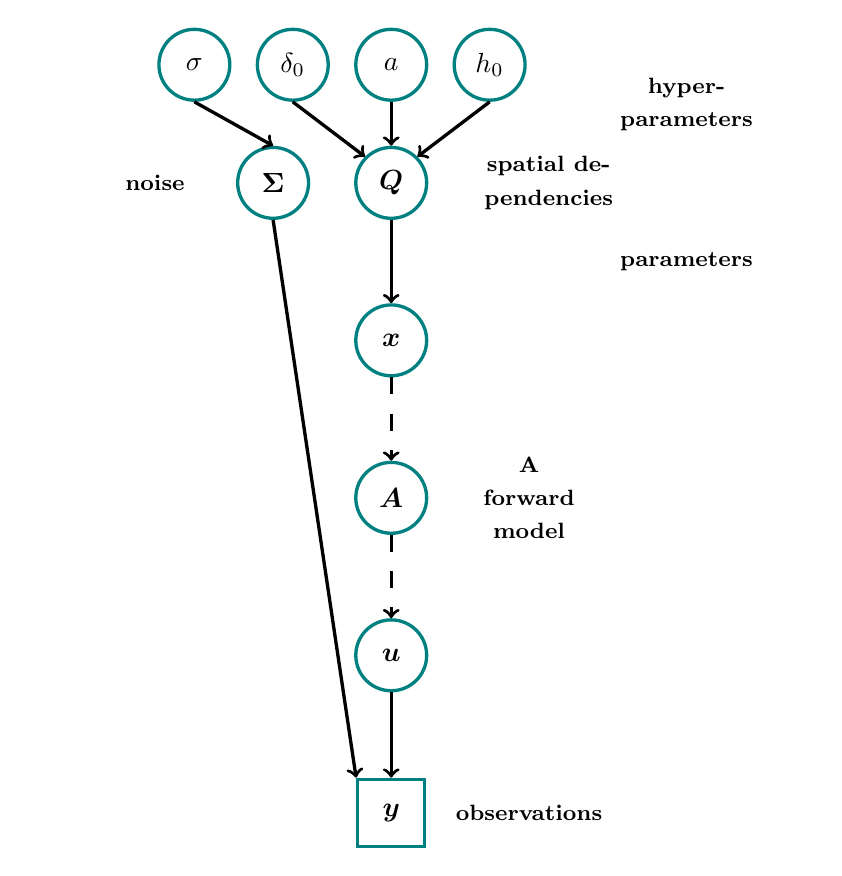
\begin{tikzpicture}
		\node[roundnode2] at (0,6) (Q)     {$\bm{Q}$};
		\node[roundnode2] at (0,4) (x)     {$\bm{x}$};
		\node[roundnode2] at (0,2) (A)    {$\bm{A}$};
		\node[roundnode2] at (0,0) (u)    {$\bm{u}$};
		\node[rectnode] at (0,-2) (y)    {$\bm{y}$};
		\node[roundnode2] at (-1.5,6) (S)    {$\bm{\Sigma}$};
		\node[roundnode2] at (-2.5,7.5) (s)    {$\sigma$};
		\node[roundnode2] at (-1.25,7.5) (d)    {$\delta_0$};
		\node[roundnode2] at (0,7.5) (a)    {$a$};
		\node[roundnode2] at (1.25,7.5) (h0)    {$h_0$};
		
		%text
		%\draw (-1,2.5) node[align=center, text width=1.5cm] {\footnotesize \textbf{hydrostatic \\ equation}};
		\draw (1.75,2) node[align=center, text width=1.5cm] {\footnotesize \textbf{A \\ forward model }};
		%\draw (6.75,-1.5) node[align=center, text width=2.5cm] {\footnotesize \textbf{hyper\-parameters}};
		%\draw (5.5,-1.5) node[align=center, text width=0.5cm] { $\bm{\theta}$};
		\draw (1.75,-2) node[align=center, text width=3cm] {\footnotesize \textbf{observations}};
		\draw (3.75,7) node[align=center, text width=3cm] {\footnotesize \textbf{hyper-\\parameters}};
		\draw (3.75,5) node[align=center, text width=3cm] {\footnotesize \textbf{parameters}};
		\draw (2,6) node[align=center, text width=3cm] {\footnotesize \textbf{spatial dependencies}};
		%\draw (-1.4,-2.3) node[align=center, text width=3cm] {\footnotesize \textbf{hyper-prior}};
		\draw (-3,6) node[align=center, text width=3cm] {\footnotesize \textbf{noise}};
		% Calligraphic brace
		%\draw[very thick, decorate,decoration = {brace}] (5,-1) --  (5,-2);
		
		%Lines
		\draw[->, very thick] (S.south) -- (y.north west);
		\draw[->, very thick] (s.south) -- (S.north);
		\draw[->, very thick] (u.south) -- (y.north);
		\draw[->, mydotted, very thick] (A.south) -- (u.north);
		\draw[->, mydotted,  very thick] (x.south) -- (A.north);
		\draw[->, very thick] (a.south) -- (Q.north); 
		\draw[->, very thick] (h0.south) -- (Q.north east); 
		\draw[->, very thick] (d.south) -- (Q.north west); 
		\draw[->, very thick] (Q.south) -- (x.north); 
		
		
	\end{tikzpicture} 
	\caption[short text]{text}
\end{figure}

\begin{itemize}
	\item  define priors
	\item how solve inverse and determinant
	\item how many steps, integrated autocorrealtion time
	\item relative error
\end{itemize}

\begin{figure}[h]
	\centering
	%\includegraphics[width=\textwidth]{DeltaSamp.png}
	\scalebox{0.66}{\input{allHistoRes.pdf_tex}}
	\caption[]{text}
	\label{fig:Results}
\end{figure}


\begin{figure}[h]
	\centering
	%\includegraphics[width=\textwidth]{DeltaSamp.png}
	\scalebox{0.66}{\input{DeltaSamp.pdf_tex}}
	\caption[]{text}
	\label{fig:Results}
\end{figure}


\begin{figure}[h]
	\centering
	%\includegraphics[width=\textwidth]{DeltaSamp.png}
	\scalebox{0.66}{\input{O3Results.pdf_tex}}
	\caption[]{text}
	\label{fig:Results}
\end{figure}



\subsection{Sampling}

\subsection{ Rosenblatt Transform}
\subsection{(Squared) Inverse Rosenblatt Transform}
\subsection{Tensor-Train Approximation}

\begin{figure}[h]
	\centering
	%\includegraphics[width=\textwidth]{DeltaSamp.png}
	\scalebox{0.66}{\input{HistSamp.pdf_tex}}
	\caption[]{TTSIRT output}
	\label{fig:Results}
\end{figure}
\begin{figure}[h]
	\centering
	%\includegraphics[width=\textwidth]{DeltaSamp.png}
	\scalebox{0.66}{\input{DeltaSIRTSamp.pdf_tex}}
	\caption[]{text}
	\label{fig:Results}
\end{figure}

\begin{figure}[h]
	\centering
	%\includegraphics[width=\textwidth]{DeltaSamp.png}
	\scalebox{0.66}{\input{SIRTO3Results.pdf_tex}}
	\caption[]{text}
	\label{fig:Results}
\end{figure}


\section{Temperature and pressure hyperameters, tt-approx}

\begin{itemize}
	\item updating scheme
\end{itemize}

\begin{figure}[thb!]
	\centering
	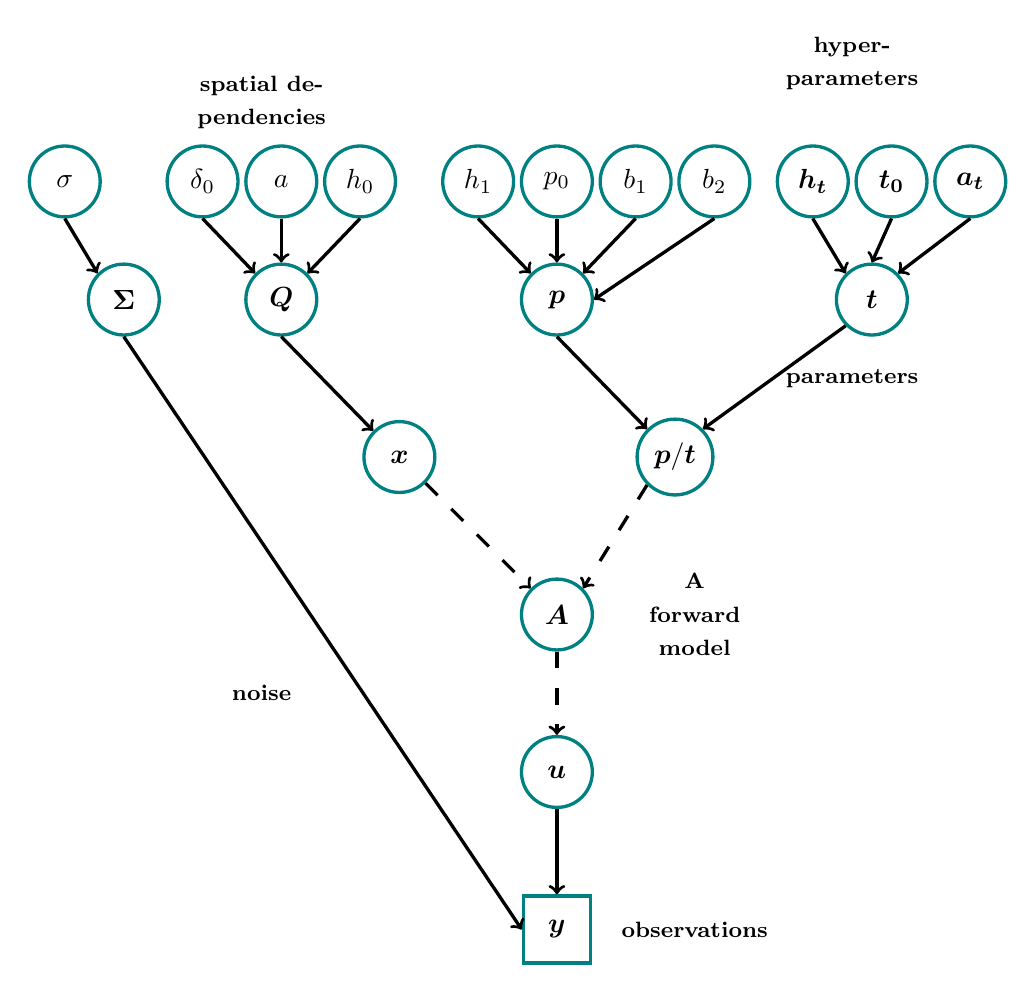
\begin{tikzpicture}
		\node[roundnode2] at (-3.5,6) (Q)     {$\bm{Q}$};
		\node[roundnode2] at (-2,4) (x)     {$\bm{x}$};
		\node[roundnode2] at (0,2) (A)    {$\bm{A}$};
		\node[roundnode2] at (0,0) (u)    {$\bm{u}$};
		\node[rectnode] at (0,-2) (y)    {$\bm{y}$};
		\node[roundnode2] at (-5.5,6) (S)    {$\bm{\Sigma}$};
		\node[roundnode2] at (-6.25,7.5) (s)    {$\sigma$};
		\node[roundnode2] at (-4.5,7.5) (d)    {$\delta_0$};
		\node[roundnode2] at (-3.5,7.5) (a)    {$a$};
		\node[roundnode2] at (-2.5,7.5) (h0)    {$h_0$};
		\node[roundnode2] at (4,6) (t)     {$\bm{t}$};
		\node[roundnode2] at (0,6) (p)     {$\bm{p}$};
		\node[roundnode2] at (1.5,4) (pt)     {$\bm{p}/\bm{t}$};
		\node[roundnode2] at (1,7.5) (b1)    {$b_1$};
		\node[roundnode2] at (2,7.5) (b2)    {$b_2$};
		\node[roundnode2] at (-1,7.5) (h1)    {$h_1$};
		\node[roundnode2] at (-0,7.5) (p0)    {$p_0$};
		\node[roundnode2] at (3.25,7.5) (ht)    {$\bm{h_t}$};
		\node[roundnode2] at (4.25,7.5) (t0)    {$\bm{t_0}$};
		\node[roundnode2] at (5.25,7.5) (at)    {$\bm{a_t}$};
		
		\draw (1.75,2) node[align=center, text width=1.5cm] {\footnotesize \textbf{A \\ forward model }};
		
		\draw (1.75,-2) node[align=center, text width=3cm] {\footnotesize \textbf{observations}};
		\draw (3.75,9) node[align=center, text width=3cm] {\footnotesize \textbf{hyper-\\parameters}};
		\draw (3.75,5) node[align=center, text width=3cm] {\footnotesize \textbf{parameters}};
		\draw (-3.75,8.5) node[align=center, text width=3cm] {\footnotesize \textbf{spatial dependencies}};
		\draw (-3.75,1) node[align=center, text width=3cm] {\footnotesize \textbf{noise}};
		
		
		%Lines
		\draw[->, very thick] (S.south) -- (y.west);
		\draw[->, very thick] (s.south) -- (S.north west);
		\draw[->, very thick] (u.south) -- (y.north);
		\draw[->, mydotted, very thick] (A.south) -- (u.north);
		\draw[->, mydotted,  very thick] (x.south east) -- (A.north west);
		\draw[->, very thick] (p.south) -- (pt.north west);
		\draw[->, very thick] (t.south west) -- (pt.north east);
		\draw[->,  mydotted, very thick] (pt.south west) -- (A.north east);
		\draw[->, very thick] (h1.south) -- (p.north west);
		\draw[->, very thick] (p0.south) -- (p.north);
		\draw[->, very thick] (b1.south) -- (p.north east); 
		\draw[->, very thick] (b2.south) -- (p.east); 
		
		\draw[->, very thick] (a.south) -- (Q.north); 
		\draw[->, very thick] (h0.south) -- (Q.north east); 
		\draw[->, very thick] (d.south) -- (Q.north west); 
		\draw[->, very thick] (Q.south) -- (x.north west); 
		\draw[->, very thick] (ht.south) -- (t.north west);
		\draw[->, very thick] (t0.south) -- (t.north);
		\draw[->, very thick] (at.south) -- (t.north east);
		
	\end{tikzpicture} 
	\caption[short text]{text}
\end{figure}

\begin{table}
	\centering
\begin{tabular}{ |c||c|c|c|   }
	\hline
	& &\multicolumn{2}{|c|}{TT bounds}\\
	\hline
	model parameters& priors&\makecell{lower\\ bound}& \makecell{upper\\ bound}\\
	\hline
	$\gamma$ & $\mathcal{T}(1,1e-4)$ &- &-\\
	$\delta$ &$\mathcal{T}(1,1e-10)$ & -&-\\
	$\gamma$ & $\mathcal{N}(2.58e-9,2.58e-11)$ &2.45e-9&2.7e-9  \\
	$\delta_0$ &  $\mathcal{N}(0.8e-4,0.75e-5)$& 4e-5 & 1.1e-4\\
	$a_0$ &  $\mathcal{T}(3,1e6)$& 1e-15&1e-5\\
	$h_0$ &  $\mathcal{N}(31.35,1)$&27 &35\\
	$h_{p,1}$ &  $\mathcal{N}(34.3,0.5)$& 32.8&35.64\\
	$p_0$ &  $\mathcal{N}(6.5,0.1)$&6.17 &6.73\\
	$b_1$ &  $\mathcal{N}(0.15,0.0051)$& 0.138  &0.167\\
	$b_2$ & $\mathcal{N}(0.13,0.067)$& 0&0.32\\
	$h_{t,0}$ &  $\mathcal{N}(11,0.5)$&9.6 &12.4\\
	$h_{t,1}$ &  $\mathcal{N}(20,3)$&11.6 &28.4\\
	$h_{t,2}$ &  $\mathcal{N}(32,1)$&29.2 &34.8\\
	$h_{t,3}$ &  $\mathcal{N}(47,2)$&41.4 &52.6\\
	$h_{t,4}$ &  $\mathcal{N}(51,2)$&45.4 &56.6\\
	$h_{t,5}$ &  $\mathcal{N}(71,2)$&65.4 &76.6\\
	$a_{t,1}$ &  $\mathcal{N}(-6.5,0.01)$&-6.528 &-6.472\\
	$a_{t,2}$ &  $\mathcal{N}(1,0.01)$&0.972 &1.028\\
	$a_{t,3}$ &  $\mathcal{N}(2.8,0.1)$&2.52 &3.078\\
	$a_{t,4}$ &  $\mathcal{N}(-2.8,0.01)$&-2.828 &-2.772\\
	$a_{t,5}$ & $\mathcal{N}(-2,0.01)$ &-2.028 &-1.972\\
	$t_{0}$ &  $\mathcal{N}(288,2)$& 282.54 &293.75\\
	\hline
\end{tabular}
\caption{Gaussian $\mathcal{N}(\mu,\sigma)$ and gamma distribution $\mathcal{T}(\alpha = \text{scale}, \beta = \text{rate})$
	Bounds for t and p 2.8 times the variance around the mean
round pressure approx and  test if would work with previous gamma prior or fix gamma prior with set values}
\label{tab:1}
\end{table}

\begin{figure}[t!]
	\centering
	\begin{subfigure}[]{.49\columnwidth}
		\centering
		\scalebox{0.42}{\input{SIRTALLTempResults.pdf_tex}}
		\caption{}
	\end{subfigure}%
	\begin{subfigure}[]{.49\columnwidth}
		\centering
		\scalebox{0.42}{\input{SIRTALLPressResults.pdf_tex}}
		\caption{}
	\end{subfigure}
	\caption{}
\end{figure}

\begin{figure}[h]
	\centering
	\scalebox{0.66}{\input{SIRTALLO3Results.pdf_tex}}
	\caption[]{text}
	\label{fig:Results}
\end{figure}



\begin{figure}[h]
	\centering
	\scalebox{0.66}{\input{PTHistSampP.pdf_tex}}
	\caption[]{complementary}
	\label{fig:Results}
\end{figure}



\begin{figure}[h]
	\centering
	\scalebox{1}{\input{PTHistSampT1.pdf_tex}}
	\caption[]{complementary}
	\label{fig:Results}
\end{figure}



\begin{figure}[h]
	\centering
	\scalebox{1}{\input{PTHistSampT2.pdf_tex}}
	\caption[]{complementary}
	\label{fig:Results}
\end{figure}



%\chapter{Application to Cube-Sat}
\label{ch:3-application}
In this chapter, we would like to introduce the Atmospheric model and how we apply this to our earlier presented sampling algorithms.
Firstly, we like to formulate the linear forward model and showcase with one specific measurement setup how we implemented the marginal and then conditional (MTC) sampler.
\mccorrect{Maybe another sampler.}
In doing so, we utilize a Metropolis within Gibbs sampler to sample hyper-parameters.
Afterward, we use the Randomize then Optimize (RTO) method to draw a sample from the conditional posterior density function.
This gives us a sample from the \mccorrect{full} posterior density.

\section{The forward model}
\label{subsec:atmosModel}
\begin{figure}[thb!]
\centering \input{figures/LIMB.pdf_tex}
\caption[The Forward model describing $n$ atmospheric layers and $m$ measurement processes.]{\textbf{The Forward model describing $n$ atmospheric layers and $m$ measurement processes.} The Cube-Sat is located at a height of $300$km, where each of the $m$ measurements is described through a tangent height $h_t$. Through the measurements we try to capture the Ozone profile, an example is displayed in light green, between $5$km and $90$km, below and above it we set the volume mixing ratio of Ozone to zero.
In order to do so we discretize the Ozone profile into $n$ atmospheric layers starting from the earth in black at ground level set to a height of $0$km.
This gives us a Markov random field with $x^{(1)}, \dots, x^{(n)}$ parameters
Along the golden line, we solve the path integral as formulated in Equation \ref{eq:pathInt} for each measurement.}
\label{fig:forModel}
\end{figure}
We introduce a linear forward model to describe the measurement process of a microwave sounder at the limb of the atmosphere, around $300$km above the ground of the earth.
Traces gases emit thermal radiation in the microwave regime, which we can capture with a resonator.
This resonator is a whispering gallery resonator, which can capture microwaves in the THz domain as well as light in the optical domain.
The microwaves are shifted towards the optical domain and we are able to read out a signal, without cooling down the measurement device.
Not needing the cooling unit allows us to fit everything we need to measure trace gases in the atmosphere into a Cube-Sat.
Depending on the angle we can measure different atmospheric layers and their traces gases, in this case, we focus on the volume mixing ratio (VMR) of Ozone $\bm{x} \in \mathbb{R}^n$.
The forward model $ \bm{F} \in \mathbb{R}^{m \times n}$  maps the Ozone profile to the space of all measurable, then can measure the data $\bm{y} \in \mathbb{R}^m$.
\begin{align}
   \bm{y} =  \bm{F}  \bm{x} + \gamma
\end{align} 

The forward model is defined through the number of atmospheric layers $n$ and measurements $m$, which are independent of each other as seen in Figure \ref{fig:forModel}.
Each measurement for a specific wavelength $\sigma$ can be described with a path integral (golden in Figure \ref{fig:forModel}) along $r$ the line of sight of the instrument, starting from $r_{obs}$, the location of the CubeSat through the atmosphere until $r_{\infty}$:
\begin{align}
\label{eq:pathInt}
     \int^{r_{\infty}}_{r_{obs}} S(\sigma) x(r) k_m(\sigma) \eta(r) \text{d}r \, ,
\end{align}
where $S(\sigma)$ is the Planck function, $\eta(r)$ number density of air, $k_m(\sigma) $ absorption cross section and $x(r)$ is the volume mixing ratio of ozone.
We assume thermal equilibrium when calculating the Planck function and discrete the atmosphere to calculate the integral.
Below a height of $5$km and above a height of $90$km, we set the volume mixing ratio of Ozone to zero.
Each measurement is defined according to a tangent height $h_t$.
The measurement is perturbed with white noise, which we describe through the hyper-parameter $\gamma$.
For further reading we refer to the Envisat MIPAS Handbook \cite{fischer2000envisat} and appendix \ref{ap:RTE}.

Based on the forward model, also displayed in figure \ref{fig:forModel}, we set up a linear-Gaussian hierarchical Bayesian model.
\begin{subequations}
    \begin{align}
        \bm{y}|\bm{x}, \gamma &\sim \mathcal{N}(\bm{F}\bm{x}, \gamma^{-1}\bm{I}) \\
        \bm{x}| \delta &\sim  \mathcal{N}( 0, (\delta \bm{L})^{-1}  ) \\
        \pi(\gamma) &\propto \gamma^{\alpha_\gamma -1} \exp{(- \beta_\gamma \gamma)} \label{eq:gamma} \\
        \pi(\delta) &\propto \delta^{\alpha_\delta -1} \exp{(- \beta_\delta \delta)} \label{eq:delta}
    \end{align}
\end{subequations}


The hyper-parameters $\gamma$ and $\delta$ are described with relatively uninformative priors.
The coefficients of the gamma distributions in Equations \ref{eq:gamma} - \ref{eq:delta} are $\alpha_\gamma = \alpha_\delta = 1 $ and $\beta_\gamma = \beta_\delta = 10^{-4}$, here we use the paper of Fox and Norton as a reference \cite{fox2016fast}.

We describe the spatial dependencies of the Ozone profile with the lumping constant $\delta$, which gives a measure of how strongly the individual parameters interact, and a graph Laplacian to describe maximum cliques and neighborhoods.
The parameters $x^{(1)}, \dots, x^{(n)}$ are normally distributed and form a Gaussian Markov random field (GMRF).
\begin{align}
    x^{(i)}| \partial x^{(i)} \sim  \mathcal{N}( |\partial^{(i)}|^{-1} \sum\nolimits_{j\in \partial x^{(i)} } x_j , (\delta |\partial^{(i)}|)^{-1}  )
\end{align}
Here $\partial x^{(i)}$ is the neighborhood of $x^{(i)}$ and $|\partial^{(i)}|$ the number of nodes connected to $x^{(i)}$ in that GMRF.
We relate the GMRF in our hierarchical Bayesian model with the precision matrix of the parameters $\bm{Q}= \delta \bm{L}$.
The Matrix L is constructed such that one parameter $x_i$ is only affected by its neighboring parameters $x_{i-1}$ and $x_{i+1}$.
We implement non-periodic boundaries.
\begin{align}
 \bm{Q}= \delta \bm{L} =
    \delta
\begin{bmatrix}
     1 & -1 & 0 & \cdots & 0\\
     -1 & 2 & -1 & \ddots & \vdots \\
     0 & \ddots & \ddots & \ddots & 0 \\ 
     \vdots & \ddots  & -1 & 2 & -1 \\
       0 & \cdots & 0 & -1 & 1 \\
\end{bmatrix}  
\end{align}

Given this setup, we can generate samples from the marginal posterior distribution $\lambda, \gamma | \bm{y}$ for the hyper-parameters $\gamma$ and $\lambda = \delta / \gamma$.
So that the marginal posterior is:
\begin{align}
    \pi(\lambda, \gamma | \bm{y})
    \propto ( \lambda \gamma)^{n/2} \exp{ \Bigg( - \frac{1}{2} g ( \lambda) - \frac{\gamma}{2} f ( \lambda) \Bigg) } \, .
    \label{eq:MargPostAppl}
\end{align}
We introduce the function $f(\lambda)$ and $g(\lambda)$ as:
\begin{subequations}
\label{eq:fandg}
\begin{align}
    f ( \lambda) &= \bm{y}^T \bm{y} - (\bm{F}^T \bm{y})^T (\bm{F}^T  \bm{F} + \lambda \bm{L})^{-1} (\bm{F}^T \bm{y})  \label{eq:f} \, \,  \text{and} \\
    g(\lambda) &= \log \det (\bm{F}^T  \bm{F} + \lambda \bm{L}) \label{eq:g}\,,
\end{align}
\end{subequations}
where $g(\lambda)$ accounts for the ratio of determinants, which is usually expensive to calculate.
We plotted those functions in Figure \ref{fig:fandg} for a large range of $\lambda$ and will use their behavior to our advantage later this in section.
%As displayed in Figure \ref{fig:fandg}, those functions behave quite well and we will use that to our advantage as we need to calculate the difference of those functions when sampling $\lambda$.

To generate a Markov chain of hyper-parameter samples we choose a so-called Metropolis-within-Gibbs algorithm, see Algorithm \ref{alg:MwG}.
We use a Metropolis-Hastings algorithm to draw $\lambda$ samples from $\pi(\lambda |  \bm{y}, \gamma )$ and then do a Gibbs step in $\gamma$ direction, where we draw a sample from the distribution \ref{eq:gammaPrior}.
\begin{subequations}
\begin{align}
    \label{eq:gammaPrior}
     \gamma |  \bm{y}, \lambda &\sim \Gamma \bigg( \frac{m}{2} + \alpha_\delta + \alpha_\gamma, \frac{1}{2} f (\lambda ) + \beta_\gamma + \beta_\delta \lambda \bigg)\\
     \label{eq:lamPrior}
     \pi(\lambda | \bm{y}, \gamma) &\propto \lambda^{n/2+\alpha_\delta -1} \exp{\bigg( - \frac{1}{2} g ( \lambda) - \frac{\gamma}{2} f ( \lambda) - \beta_\delta \gamma \lambda \bigg)}
\end{align} 
\end{subequations}
If we like to utilize a Metropolis-Hastings algorithm on the probability density Function \ref{eq:lamPrior} we need to evaluate the Ratio \ref{eq:lamRatio}, to do a step in $\lambda + \Delta \lambda $ direction and to generate a new candidate $\lambda'$.
\begin{align}
\label{eq:lamRatio}
    \frac{\pi(\lambda' |  \bm{y}, \gamma ) }{\pi(\lambda |  \bm{y}, \gamma) } \propto \bigg(\frac{\lambda'}{\lambda}\bigg)^{n/2+\alpha_\delta -1} \exp \bigg( -& \frac{1}{2} \big(  g ( \lambda') - g ( \lambda) \big) \\  -& \frac{\gamma}{2} \big( f ( \lambda') - f ( \lambda) \big)- \beta_\delta \gamma (\lambda' - \lambda) \bigg)
\end{align}
This comes down to evaluating the difference $f ( \lambda') - f ( \lambda)$ and $g ( \lambda') - g ( \lambda) $ efficiently.
Within a small change of $\lambda' = \lambda + \Delta \lambda$, those functions are well-behaved, as we can see in Figure \ref{fig:fandg}.
Then we approximate those functions with a Taylor series:
\begin{align}
    f^{(r)} (\lambda)=& (-1)^{r+1} r! (\bm{F}^T \bm{y})^T (\bm{B}^{-1} \bm{L})^r \bm{B}^{-1} \bm{F}^T \bm{y} \label{eq:ftay} \\
    g^{(r)} ( \lambda) =&  (-1)^{r+1} \, \text{tr} \big( (\bm{B}^{-1}\bm{ L })^r \big) \, ,
   % =& \mathbb{E} [ z^T (\bm{B}^{-1} \bm{L} )^r z ] , \quad \text{where } \, z_i \overset{\text{i.i.d.}}{\sim} \mathcal{U} ( \{ -1, 1 \} ) \, ,
   \label{eq:gtay}
\end{align} 
where $\bm{B} = \bm{F}^T  \bm{F} + \lambda \bm{L}$,\mccorrect{for more details we refer to the Appendix} \ref{ap:taylor}.
Hence we use the Taylor approximations to evaluate the difference of the functions $f(\lambda)$ and $g(\lambda)$ for a small change $\Delta \lambda = \lambda' - \lambda$ we rewrite the ratio:
\begin{align}
    \frac{\pi(\lambda' | \bm{y}, \gamma ) }{\pi(\lambda |\bm{y},  \gamma ) } \propto \bigg(\frac{\lambda'}{\lambda}\bigg)^{n/2+\alpha_\delta -1} \exp \bigg( - \frac{1}{2}& \bigg[  \sum_{r=1}^{2} \bigg( \frac{g^{(r)}( \lambda)}{r!}  + \gamma  \frac{f^{(r)}( \lambda)}{r!}  \bigg)  (\lambda' - \lambda)^{(r)} \bigg] \\ -& \beta_\delta \gamma (\lambda' - \lambda) \bigg) \, .
\end{align}
Now, we are able to generate a Markov chain of hyper-parameter samples \newline$ \{ (\lambda, \gamma )_{1}, \dots ,(\lambda, \gamma )_{1 + \tau_{\text{int}} }, \dots ,(\lambda, \gamma )_{1+K \tau_{\text{int}} }, \dots ,(\lambda, \gamma )_{K'}\}$.
Lastly, we refine the chain according to the integrated auto-correlation time $\tau_{\text{int}}$, so that $K < K'$ independent hyper-parameter samples characterize the marginal posterior distribution.


Finally, we sample the parameter $x_i |  \bm{y}, \lambda_i, \gamma_{i} $ conditioned on the hyper-parameters $(\lambda_i, \gamma_{i})$ and the data $\bm{y}$.
To do so, we pick one $(\lambda, \gamma )_{i} \in \{(\lambda, \gamma )_{1}, (\lambda, \gamma )_{2} ,\dots ,(\lambda, \gamma )_{K}\} \sim \pi(   \lambda, \gamma | \bm{y} )$ and generate a parameter sample by solving the following equation:
\begin{align}
\label{eq:RTOapplied}
    (\gamma_i \bm{F}^T  \bm{F}+
    \delta_i \bm{L} ) \bm{x}_i &= \gamma_i \bm{F}^T \bm{y} + \bm{v}_1 + \bm{v}_2 \,  ,
\end{align}
where we draw two independent random variables $\bm{v}_1 \sim \mathcal{N}(\bm{0}, \gamma_i \bm{F}^T  \bm{F}) $ and $\bm{v}_2 \sim \mathcal{N}(\bm{0}, \delta_i \bm{L} )$.


\begin{algorithm}[thb!]
    \caption{Metropolis-within-Gibbs step to generate hyper-parameter samples}
    \label{alg:MwG}
    \SetAlgoLined
    \nonl
    \textbf{Generate}: $\{ (\lambda, \gamma )_{1}, \dots ,(\lambda, \gamma )_{j+1}, \dots ,(\lambda, \gamma )_{K'}\}$\\
    \ForEach{$(\lambda, \gamma )_{j} = (\lambda, \gamma )$}{
        \textbf{Propose} new state: $  \lambda' \sim  g(\lambda'|\lambda )$ \\
    \textbf{Acceptance probability}: $
      \alpha (\lambda'|\lambda) \equiv \min 
    \begin{rcases}
        \begin{dcases}
            1,       \frac{\pi(\lambda' |  \bm{y}, \gamma ) g(\lambda|\lambda')}{\pi(\lambda |  \bm{y}, \gamma ) g(\lambda'|\lambda) } 
        \end{dcases}
    \end{rcases} $ \\
    \textbf{Draw}: $ u \sim \mathcal{U}(0,1)$ \\ 
    {\If{$u \leq \alpha (\lambda'|\lambda)$,}{
    \textbf{Accept}: $ \lambda' $\;
    \lElse{ \textbf{Reject}:  $\lambda ' = \lambda$}}}
    \textbf{Draw}: $     \gamma' |  \bm{y}, \lambda' \sim \Gamma \Bigg( \frac{m}{2} + \alpha_\delta + \alpha_\gamma, \frac{1}{2} f (\lambda') + \beta_\gamma + \beta_\delta \lambda' \Bigg)$\\
     \textbf{Set}: $(\lambda, \gamma )_{j+1}$ = $(\lambda', \gamma' )$\\}
    \textbf{Calculate}: integrated auto-correlation time $\tau_{\text{int}}$ for large enough $K'$\\
    \textbf{Refine chain} according to $\tau_{int}$ so that $   \{(\lambda, \gamma )_{1}, (\lambda, \gamma )_{2} ,\dots ,(\lambda, \gamma )_{K}\} \sim \pi(   \lambda, \gamma | \bm{y} )$, where $ K < K'$
\end{algorithm}
\clearpage

\section{Results}
\label{sec:Results}
In this section, we present the results for one specific measurement setup with a set Ozone profile and number of layers.
We compare the MTC-Sampler against the T-Walk algorithm \cite{christen2010general}.

\begin{figure}[htb]
\centering
\includegraphics[width=1\textwidth]{OxThesis-master/figures/f_and_g.png} 
\caption[Plotting $f(\lambda)$ and $g(\lambda)$ for a large range of $\lambda$ to characterize the marginal posterior distribution.]{\textbf{Plotting $f(\lambda)$, Eq. \ref{eq:gtay}, and $g(\lambda)$, Eq.m \ref{eq:gtay}, for a large range of $\lambda$ to characterize the marginal posterior distribution.}
We included the samples mean of the MTC-Sampling (red) and T-walk algorithm (black) \cite{}. In the upper left corner of each figure, we plotted the Taylor series (red) of $f(\lambda)$ and $g(\lambda)$ around the mode of the marginal posterior $\pi(\delta_0, \gamma_0 | \bm{y})$, where $\lambda_0 = \delta_0 / \gamma_0 $. To display the Taylor series we computed up to the fifth derivatives of each function. Note that we usually only focus on a small range of $\lambda$ compared to the here shown range.}
\label{fig:fandg}
\end{figure}
In doing so we set up a specific forward model, in which we specify the number of layers and the number of measurements, to determine the Equations \ref{eq:gammaPrior} and \ref{eq:lamPrior}.
We measure $m = 105$ times equally spaced in between the tangent heights of $2$km and $100$km.
We were given data of $n = 47$ Ozone layers so that the Ozone concentration is zero below 5km and above 90km, as indicated in Figure \ref{fig:forModel}.
We stimulated white noise with a standard deviation of 1\% of the maximum value of data and plotted this in golden color in see Figure \ref{fig:RecRes}.
We calculate the function $f(\lambda)$ and $g(\lambda)$ by using the linear solver \textit{gmres} of the \textit{scipy.sparse.linalg} package in \textit{Python}.
We use the solver to compute the matrix multiplication of $\bm{B}^{-1}\bm{L}$ and $\bm{B}^{-1} \bm{F}^T \bm{y}$, where we set the tolerances for convergence to $10^{-7}$ and repeat the process after 25 iterations.
For a large range of $\lambda$ we plotted $f(\lambda)$ and $g(\lambda)$ in Figure \ref{fig:fandg} and include some results of the sampling process such as sample mean of the MTC-Sampler in red and of the T-Walk algorithm in black.
The top left corner of each figure shows the Taylor approximation around the mode of the marginal posterior distribution in red underneath the original function in blue.

\begin{figure}[thb]
 \begin{subfigure}{0.5\textwidth}
     \centering
     \includegraphics[width=\textwidth]{OxThesis-master/figures/HistoResults.png}
     \caption{}
     \label{fig:MTCHisto}
 \end{subfigure}
 \hfill
 \begin{subfigure}{0.5\textwidth}
     \centering
     \includegraphics[width=\textwidth]{OxThesis-master/figures/PyTWalkHistoResults.png}
      \caption{}
     \label{fig:TWalkHisto}
 \end{subfigure}
\caption[Sampling Results of the MTC-Sampler and the T-Walk algorithm \ref{fig:TWalkHisto}]{\textbf{Sampling Results of the MTC-Sampler \ref{fig:MTCHisto} and the T-Walk algorithm \ref{fig:TWalkHisto}.} The histograms present independent samples of the marginal posterior distribution according to their integrated Auto-correlation time $\tau_{int}$.
Using the \textit{UWerr.m} function by U. Wolff we calculate integrated auto-correlation times of $\tau_{\text{int}, \text{MTC}, \gamma} = 5.4$, $\tau_{\text{int}, \text{MTC}, \delta} = 4.9$ and $\tau_{\text{int}, \text{MTC}, \lambda}= 10.2$ when utilizing the MTC-Sampler with an acceptance rate of 0.34 \cite{Uwerr}.
Running the T-Walk algorithm we obtain following auto-correlation times: $\tau_{\text{int}, \text{T-walk}, \gamma} = 34.1$, $\tau_{\text{int}, \text{T-walk}, \delta} = 34.5$ and $\tau_{\text{int}, \text{T-walk}, \lambda}= 27.5$, with an acceptance rate of 0.42.}
\label{fig:histRes}
\end{figure}
Next, we found the mode at $(\gamma_0, \delta_0) = (1 \times 10^{-5}, 0.26)$ of the marginal posterior distribution by using the \textit{optimize.fmin} function from the \textit{scipy} package in \textit{Python}.
In Figure \ref{fig:fandg} this mode is indicated in green and is the value where we initialize our Markov chain.
We use a normal proposal distribution so that $\lambda' | \lambda \sim \mathcal{N}(\lambda| w^2_{\lambda})$ and draw $10^4$ samples of the marginal posterior distribution, with a burn in period of 50 samples.
We tune variance of the proposal distribution so that the acceptance ratio is between 0.25 and 0.5, and set $w_{\lambda} = 5\times 10^3$.
After calculating the auto-correlation times with \textit{MATLAB} function \textit{UWerr.m} by Ulli Wolff we calculate integrated auto-correlation times \cite{Uwerr}.
Note that we use two times the values of the output of that function, as indicated in \cite{fox2016fast}.
Given the integrated auto-correlation times, we can generate independent samples of the marginal posterior distribution $\pi(\lambda, \gamma | \bm{y})$, see Figure \ref{fig:histRes}.
The integrated auto-correlation times of the MTC-Sampler are: $\tau_{\text{int}, \text{MTC}, \gamma} = 5.4$, $\tau_{\text{int}, \text{MTC}, \delta} = 4.9$ and $\tau_{\text{int}, \text{MTC}, \lambda}= 10.2$.
This is significantly lower compared to the T-Walk algorithm, which needs more than 34 samples to draw two independent hyper-parameter values.
\mccorrect{We indicated the sample mean in Figure} \ref{fig:fandg}\mccorrect{and would like to point out that the T-walk algorithm hits the precalculated mode of the marginal posterior quite accurately.
The MTC-Sampler seems to have a bigger $\gamma$ sample mean compared to the true value.
This reduces the value of $\lambda$ from around $2 \times 10^5$ to $5 \times 10^4$.}

\begin{figure}[htb]
\centering\includegraphics[width=0.7\textwidth]{OxThesis-master/figures/FirstRecRes.png} 
\caption[Randomize then Optimize (RTO) method to recover the Ozone profile in dependency of the height.]{\textbf{Randomize then Optimize (RTO) method to recover the Ozone profile in dependency of the height.} Here we plotted the mean of 10 posterior samples and their variance in red. We draw hyper-parameter samples according to the samples seen in Figure \ref{fig:MTCHisto}. In green, we displayed the true Ozone profile $\bm{x}$.
We show the data $\bm{y}$ including noise in golden for each tangent height.}
\label{fig:RecRes}
\end{figure}
Given the samples obtained by the MTC-Sampler, see Figure \ref{fig:MTCHisto}, we draw hyper-parameters from the marginal posterior accordingly.
The Randomize then Optimize (RTO) method allows us to compute parameter samples from the full posterior $\pi(\bm{x},\lambda, \gamma|\bm{y})$.
We solve Equation \ref{eq:RTOapplied} for 10 independent hyper-parameter samples to obtain 10 parameter samples.
We plot the results in Figure \ref{fig:RecRes}, where the red line indicates the sample mean including the sample variance.
The results match up well with the true Ozone profile plotted in green.
We included the data $\bm{y}$ in dependency of the tangent height in golden color.

%######################### ideas #####################

% The main goal of this thesis is to apply the introduced samplers to atmospheric trace gas measurements.
% Here we introduce a atmospheric model first a linear model and then raise complexity for the non-linear case.
% The model is suitable to describe a measurement process for a LIMB-Sounder

% \mccorrect{Maybe at the beginning.. or mention at the beginning that this is the motivation for this work.. speed up sampling.. can we deliver real time data?}

% \begin{itemize}
%     \item figure of atmosphere
%     \item Limb sounder - basic principles
%     \item linear model
%     \item non linear model
% \end{itemize}



% -how to sep up a model
% - scaling of the froward map and scaling
% -hyperparameter
% -sample from hyperpriors



%\chapter{Nonlinear Forward model}
\begin{itemize}
	\item updating scheme, slow
	\item local linear map, strategy, schematic
	\item affine function, RTO
\end{itemize}

\section{Sampling}

\begin{figure}[h]
	\centering
	\includegraphics[width=\textwidth]{NonLinFirstRecRes.png}
	\caption[]{text}
	\label{fig:Results}
\end{figure}

\section{local linear Map and strategy}

\subsection{Machine learning vs Gaussian elimination}

\section{affine RTO}
%\chapter{Introduction}
\section{Motivation}
\begin{itemize}
	\item Ozone coverage
	\item Cube Sat is built
	\item existing inversion methods based on regularization
\end{itemize}

\section{What is going on?, 3 facts, What is new in this thesis?}
\begin{itemize}
	\item RTE as an hierachical Bayesian model
	\item nonLinear to Linear Affine funciton (affine RTO)
	\item sampling to TT approx
\end{itemize}

\section{What has been published?}
%% APPENDICES %% 
% Starts lettered appendices, adds a heading in table of contents, and adds a
%    page that just says "Appendices" to signal the end of your main text.
\startappendices
% Add or remove any appendices you'd like here:
%\chapter{Posterior of Bayesian Hierachical model}
\label{ap:bayesian}
Here we show how to obtain the posterior covariance and mean of our hierarchical Bayesian model in \ref{eq:prior} - \ref{eq:post}.
We do not consider the hyper-parameters and start with the joint probaility distribution of $(\bm{x}^T,\bm{y}^T)^T$, where $\bm{x} \in \mathcal{X}$ and $\bm{y} \in \mathcal{Y}$ do not intersect.
For more details we refer to Chapter 2 in \cite{bishop2006pattern} and to the book of Rue and Held \cite{rue2005gaussian}.

The exponent of the normal Gaussian can be rewritten into:
\begin{align}
\label{eq:gauss}
    -\frac{1}{2}(\bm{x} - \bm{\mu})^T \bm{Q} (\bm{x} - \bm{\mu}) = - \frac{1}{2} \bm{x}^T \bm{Q} \bm{x} + \bm{x}^T \bm{Q} \bm{\mu} + \text{const.}
\end{align}
We like to bring the joint distribution into a similar form so that we can compare the linear and second order terms and find the precision matrix and mean of the joint distribution.


In general the joint distribution to find the experssino for the postiror dostrbution

We can express this posterior through the likelihood and prior probability by Bayesian theorem, with a constant and positive normalization constant:
\begin{equation}
    \pi(\bm{x} |\bm{y}) \propto \pi( \bm{y} | \bm{x} )  \pi(\bm{x} )
\end{equation}
Taking the logarithmic function of this formulation we can find an expression for the the posterior covariance, with the $\text{Var}(\bm{x}) = \bm{Q_x}^{-1}$ and $\text{Var}(\bm{y}) = \bm{Q_y}^{-1}$.
\begin{align}
\ln{\pi(\bm{x|y})} \propto&  \ln{ \pi( \bm{y} | \bm{x} ) } + \ln{\pi( \bm{x} ) }\\
=& - \frac{1}{2} (\bm{x} - \bm{\mu} )^T \bm{Q_x} (\bm{x} - \bm{\mu} ) - \frac{1}{2} (\bm{y} - \bm{Ax} )^T \bm{Q_y} (\bm{y} - \bm{Ax} )    \\
=& - \frac{1}{2} \bigg[ \bm{x}^T \big[ \bm{Q_x} + \bm{A}^T \bm{Q_y} \bm{A} \big] \bm{x}  + \bm{x}^T \big[ - \bm{A}^T \bm{Q_y} \big] \bm{y} \\
&+ \bm{y}^T \big[ - \bm{Q_y A} \big] \bm{x} + \bm{y}^T \big[ \bm{Q_y} \big] \bm{y} - 2 \bm{x}^T \bm{Q_x \mu }  \bigg] + \text{const.}
\end{align}

Hence we deal with a Gaussian distribution, we consider second order terms only and rearrange to the precision matrix.
\begin{align}
    &- \frac{1}{2} \begin{bmatrix}
        \bm{x}^T \big[ \bm{Q_x} + \bm{F}^T \bm{Q_y} \bm{F} \big]  + \bm{y}^T \big[ - \bm{Q_y F} \big] & \bm{y}^T \big[ \bm{Q_y} \big] + \bm{x}^T \big[ - \bm{F}^T \bm{Q_y} \big] 
    \end{bmatrix}  \begin{bmatrix}
        \bm{x} \\ \bm{y}
    \end{bmatrix} \\
    =& \begin{bmatrix}
        \bm{x}^T & \bm{y}^T
    \end{bmatrix} 
    \underbrace{\begin{bmatrix}
        \bm{Q}_x + \bm{F}^T \bm{Q}_y \bm{F} & - \bm{F}^T \bm{Q}_y \\
        -\bm{Q}_y \bm{F} & \bm{Q}_y
    \end{bmatrix}}_\text{precision matrix} \begin{bmatrix}
        \bm{x} \\ \bm{y}
    \end{bmatrix} 
\end{align}
We denote the precision matrix of the joint field as:
\begin{align}
    \bm{Q}_{xy} = \begin{bmatrix}
        \bm{Q}_{aa} & \bm{Q}_{ab} \\
        \bm{Q}_{ba} & \bm{Q}_{bb}
    \end{bmatrix} = 
    \begin{bmatrix}
        \bm{Q}_x + \bm{F}^T \bm{Q}_y \bm{F} & - \bm{F}^T \bm{Q}_y \\
        -\bm{Q}_y \bm{F} & \bm{Q}_y
    \end{bmatrix}
\end{align}

The mean is defined through the linear term.
\begin{align}
    \frac{- 2 \bm{x}^T \bm{Q_x \mu } }{-2} = \begin{bmatrix}
        \bm{x}^T & 0
    \end{bmatrix} \begin{bmatrix}
        \bm{Q_x \mu}\\ 0
    \end{bmatrix} 
    \end{align} 
Comparing to the linear term of Equation \ref{eq:gauss} we can formulate an expression for the joint mean:
    \begin{align}
    \Rightarrow \bm{\mu_{xy}} = \bm{Q}_{\bm{x}\bm{y}}^{-1}   \begin{bmatrix}
        \bm{Q_x \mu}\\ 0
    \end{bmatrix}
\end{align}
The mean of the conditional distribution $\bm{x}|\bm{y}$ is given by:
\begin{align}
\bm{\mu}_{\bm{x}|\bm{y}} &= \bm{\mu}_{\bm{x}} + \bm{Q}^{-1}_{ba} \bm{Q}_{ab} (\bm{x} - \bm{\mu}_{\bm{y}}) \\
\bm{\mu}_{\bm{x}|\bm{y}} &= \bm{\mu} +  ( \bm{Q}_x + \bm{F}^T \bm{Q}_y \bm{F} )^{-1} \bm{F}^T \bm{Q}_y ( \bm{x} - \bm{F \mu} ) \, ,
\end{align}
and the covariance of $\bm{x}|\bm{y}$ is given by:
\begin{align}
   \bm{Q}_{\bm{x}|\bm{y}} =  \bm{Q}_{aa} = \bm{Q}_x + \bm{F}^T \bm{Q}_y \bm{F} \, ,
\end{align}
as illustrated through Theorem 2.5 in \cite{rue2005gaussian}.


\chapter{Convergence of the Metropolis-Hastings}
\label{ap:MetroHast}

If we show that the detailed balance condition holds and that the state space is irreducible and aperiodic under the transition matrix $\bm{P}$, we generate a Markov chain with a unique stationary distribution proportional to $\pi (\bm{x} , \bm{\theta} | \bm{y})$.
Since the posterior is strictly positive $\pi (\bm{x} , \bm{\theta} | \bm{y}) \geq 0$ on the finite state space $\Omega(\mathcal{X},\mathcal{\theta})$ the generated chain is irreducable.
Further, it is possible to reject any proposed state and stay in the current state, which leads to aperiodicity.
The detailed balance holds for the case that $\bm{j} = \bm{i}$, but if $\bm{j} \neq \bm{i}$ it is not trivial.
In case we accept $\{ \bm{x}, \bm{\theta} \}^{(n+1)} = \bm{j}$ as the new state we have $ \pi(\bm{j} | \bm{y})  g(\bm{i}|\bm{j})> \pi(\bm{i} | \bm{y})  g(\bm{j}|\bm{i})$.
This gives us $\alpha(\bm{j}|\bm{i}) = 1$ and $\alpha(\bm{i}|\bm{j}) = \frac{\pi_{\bm{i}} g(\bm{j}|\bm{i})}{\pi_{\bm{j}} g(\bm{i}|\bm{j})}$ and satisfies the detailed balance:
\begin{align*}
    \cancel{\pi_{\bm{j}}}  \frac{\pi_{\bm{i}}}{\cancel{\pi_{\bm{j}}}} g(\bm{j}|\bm{i}) &= \pi_{\bm{i}} g(\bm{j}|\bm{i}) \quad .
\end{align*}
If $ \pi(\bm{j} | \bm{y})  g(\bm{i}|\bm{j}) < \pi(\bm{i} | \bm{y})  g(\bm{j}|\bm{i})$ then $\alpha(\bm{i}|\bm{j}) = 1$
and $\alpha(\bm{j}|\bm{i}) = \frac{\pi_{\bm{j}} g(\bm{i}|\bm{j})}{\pi_{\bm{i}} g(\bm{j}|\bm{i})}$, this satisfies the detailed balance as well.

In conclusion the Metropolis-Hastings algorithm samples from a unique distribution proportional to the posterior distribution. 

\chapter{Randomize then Optimize - RTO}
\label{ap:RTO}

\begin{align}
    \pi(\bm{x}|\bm{y}, \bm{\theta} ) &\propto \pi(\bm{y} | \bm{x} , \bm{\theta} ) \pi(\bm{x}| \bm{\theta}) \\
   &\propto \exp \Big[  ( \bm{F x} - \bm{y})^T \bm{\Sigma}^{-1}( \bm{F x} - \bm{y}) + (\bm{x} -\bm{\mu} )^T \bm{Q} (\bm{x} -\bm{\mu})\Big] \\
   &= \exp  \lVert \hat{\bm{F}} \bm{x} - \hat{\bm{y}} \rVert^2 
\end{align}
where 
\begin{align}
\hat{\bm{F}} = 
    \begin{bmatrix}
         \bm{\Sigma}^{-1/2} \bm{F}\\
    \bm{Q}^{1/2}
    \end{bmatrix} \, , \quad \hat{\bm{y}} = 
    \begin{bmatrix}
        \bm{\Sigma}^{-1/2} \bm{y} \\
        \bm{Q}^{1/2}\bm{\mu}
    \end{bmatrix}
\end{align}

One sample from the posterior can be computed by minimizing the following with respect to $\bm{x}$
\begin{align}
    \bm{x} = \arg \min_{\hat{\bm{x}}} \lVert \hat{\bm{F}} \hat{\bm{x}} - ( \hat{\bm{y}} + \bm{\eta} ) \rVert^2 , \quad \bm{\eta} \sim \mathcal{N}(\bm{0}, \mathbf{I})
\end{align}

We can solve this and rewrite to
\begin{align}
    \frac{\partial}{\partial \bm{x} }  \big[   (\hat{\bm{F}} \bm{x} - ( \hat{\bm{y}} + \bm{\eta} )^T (\hat{\bm{F}} \bm{x} - ( \hat{\bm{y}} + \bm{\eta} ) \big] &= 0 \\
    \Leftrightarrow \bm{x}^T \hat{\bm{F}}^T  \hat{\bm{F}} + \hat{\bm{F}}^T \hat{\bm{F}} \bm{x} -  \hat{\bm{F}}^T ( \hat{\bm{y}} + \bm{\eta} )- ( \hat{\bm{y}} + \bm{\eta} )^T  \hat{\bm{F}} \bm{x}  &= 0
\end{align}
We can argue through the symmetry of the inner product that and the symmetry of the precision matrix
\begin{align}
    \hat{\bm{F}}^T \hat{\bm{F}} \bm{x} &= \hat{\bm{F}}^T ( \hat{\bm{y}} - \bm{\eta}) \\
    \Leftrightarrow  (\bm{F}^T \bm{Q_y} \bm{F}+
    \bm{Q} ) \bm{x} &= \bm{F}^T \bm{Q_y} \bm{y} +  \bm{Q} \bm{\mu} - \hat{\bm{F}}^T  \bm{\eta}  
\end{align}
If we substitute $ - \hat{\bm{F}}^T  \bm{\eta}  = \bm{v}_1 + \bm{v}_2$ we end up with 
\begin{align}
    (\bm{F}^T \bm{\Sigma}^{-1} \bm{F}+
    \bm{Q} ) \bm{x} &= \bm{F}^T \bm{\Sigma}^{-1} \bm{y} +  \bm{Q} \bm{\mu} + \bm{v}_1 + \bm{v}_2
\end{align}
where $\bm{v}_1 \sim \mathcal{N}(\bm{0}, \bm{F}^T \bm{\Sigma}^{-1} \bm{F}) $ and $\bm{v}_2 \sim \mathcal{N}(\bm{0}, \bm{Q} )$ are independent random variables.
mayeb introduce... $x^2$ time nomral variubale


\chapter{Inverting Matrices - QR factorization}


\chapter{Taylor expansion of  $g(\lambda)$}
\label{ap:taylor}
We Taylor expand the function $g(\lambda)$ around $\lambda = \lambda'  - \Delta \lambda$
\begin{align}
    g(\lambda) = \ln \det \underbrace{(\bm{F}^T  \bm{F} + \lambda \bm{L})}_{\bm{B}}
\end{align}
\begin{align}
       g(\lambda') -    g(\lambda) &=  \ln \det ( \bm{F}^T  \bm{F} + \lambda' \bm{L}) -  \ln \det (\bm{F}^T  \bm{F} + \lambda \bm{L}) \\
    &=  \ln \det \Bigg[ \frac{(\bm{F}^T  \bm{F} + (\lambda + \Delta \lambda) \bm{L}) }{ ( \bm{F}^T  \bm{F} + \lambda \bm{L}) } \Bigg]  \\
       &=  \ln \det \Bigg[ 1 + \frac{ \Delta \lambda \bm{L} }{ \bm{B} } \Bigg]\\
       & = \sum_{r = 1}^{\infty} \frac{(-1)^{r+1}}{r !}\text{tr} (   (\bm{B}^{-1}  \bm{L} )^r  )  (\Delta \lambda)^r
\end{align}, where we use the identity from \cite{gohberg2012traces} at page 29.
So the derivatives of $g(\lambda)$ are:
\begin{align}
    g^{(r)} ( \lambda) =&  (-1)^{r+1} \, \text{tr} \big( (\bm{B}^{-1}\bm{ L })^r \big)\\
\approx& (-1)^{r+1} \sum^p_{k=1} \bm{z_k}^T (\bm{B}^{-1} \bm{L} )^r \bm{z_k}  
\end{align} 
Here we use a Monte Carlo estimate and draw $p$ vectors $\bm{z_k} \in \mathbb{R}^n $, where each vector element $z_i \overset{\text{i.i.d.}}{\sim} \mathcal{U} ( \{ -1, 1 \} )$ and $i = 1 , \dots, n$.

\chapter{Radiation transfer and absorption line shape}
\label{ap:RTE}


\chapter{whispering gallery resonator}
\label{ap:resonator}


\begin{figure}
\centering\includegraphics[width=0.7\textwidth]{GaAs_setup4.png} 
\caption[whispering gallery resonator]{whispering gallery resonator}
\label{fig:GaAsRes}
\end{figure}
\chapter{Correlation Structure}
\label{ap:Correlatation}
The book by Rue and Held shows the correlation structur between the hyperparameter $\mu$ and the laten field $\bm{x}$
We consider the hierarchal formuation 
\begin{align}
	\mu \sim \mathcal{N}(0,1)\\
	\bm{x}|\mu \sim \mathcal{N}(\mu\bm{1},\bm{Q}^{-1})
\end{align}
Gibbs sampler Since both full conditional
\begin{align}
	\mu^{(k)} | \bm{x}^{(k)} &\sim \mathcal{N} \Bigg(\frac{\bm{1}^T\bm{Q}\bm{x}^{(k-1)}}{1 + \bm{1}^T\bm{Q}\bm{1}}, (1 + \bm{1}^T\bm{Q}\bm{1})^{-1} \Bigg)\\
	\bm{x}^{(k)} | \mu^{(k)} &\sim \mathcal{N} (	\mu^{(k)}\bm{1}, \bm{Q}^{-1})
\end{align}

\begin{figure}[ht!]
	\centering
	
	\caption[Correlation structur]{Figure 4.1 Figure (a) shows the marginal chain for µ over 1000 iterations of
		the marginal chain for the hyperparmeter with a specuifuc autoregressive proces defined in $\bm{Q}$ The algorithm
		updates successively $\mu$ and $x$ from their full conditionals. Figure (b) displays
		the pairs ($\mu(k)$ ,  $1^T\bm{Q}x(k)$ ), with$\mu(k)$ on the horizontal axis. The slow mixing
		(and convergence) of $\mu$is due to the strong dependence with $1^T\bm{Q}x(k)$  as only
		horizontal and vertical moves are allowed. The arrows illustrate how a joint
		update can improve the mixing (and convergence)}
	\label{fig:FirstDAG}
\end{figure}

Our solution is to update $(\mu, x)$ jointly, where effectefally the 

Note that only the marginal density of µ is needed in (4.6): Since we
sample x from its full conditional, we effectively integrate x out of the
joint density $\pi(\mu, x)$.


\chapter{Mesure theroy}
\label{ap:Correlatation}
Recall that Asumme that the triple $(\Omega, \mathcal{F} , \mathbb{P})$ is called a probability space over the whole sample space $\Omega$ with the collection $\mathcal{F}$ of very countable subset $\{ A _n \}_{n\in \mathbb{N}}$, where a Event $A_n$ is a subset of $\Omega$, $A_n \subseteq  \Omega$, and a map $\mathbb{P} : \mathcal{F} \longrightarrow \mathbb{R}$. 
We assume $\mathbb{P}$ fullfils probality measure and  $\mathcal{F}$ is a $\sigma $-algebra see Appendix \ref{}.
We call $\mathbb{P}(A)$ the probaility of an event $A \subseteq \mathcal{F}$ 
\section{sigma alrgbea}
A collections of subsets $\mathcal{F}$ is called sigma algreab if
\begin{itemize}
	\item $\emptyset, \Omega \in \mathcal{F} $
	\item if $A \in \mathcal{F} $ then $A^C \coloneqq A / \Omega \in A$
	\item if $A_1 , A_2, \dots  \in \mathcal{F} $ then $ \bigcup_{j=1}^{\infty} A_j \in A$
\end{itemize}
\section{probailty measure}

a probailty measure has to full fil the folowing criterion 
\begin{itemize}
	\item $\mathbb{P}(\Omega) = 1$ and $\mathbb{P}(\emptyset) = 1$
	\item $\mathbb{P}(A) \in [0,1]$
	\item $\mathbb{P}(A \cup B) =\mathbb{P}(A) + \mathbb{P}(B) $ if $A, B$ are disjoint or $A\cap B = \emptyset$
	\item $\mathbb{P}(\bigcup_{j = 1}^{\infty} A_j) = \sum_{j=1}^{\infty} \mathbb{P}(A_j)$ if we have pairwise dijoint sets or $A_i \cap A_j = \emptyset$ for $i \neq j $
\end{itemize}


%%%%% REFERENCES\\


{\renewcommand*\MakeUppercase[1]{#1}%
\printbibliography[heading=bibintoc,title={\bibtitle}]}


\end{document}
